% vim: spelllang=fr

\documentclass[../main.tex]{subfiles}
\graphicspath{{\subfix{../Figures/Chap1/}}}
\begin{document}

\begin{itshape}
Ce premier chapitre introduit les cyclones tropicaux (TC), de la simple définition jusqu'à la formulation de la question scientifique présentée dans cette thèse, en introduisant tous les concepts intermédiaires nécessaires.
\end{itshape}

\minitoc\newpage
%------------------------------------------------------------------------------------------------------------------
\section{Introduction aux cyclones tropicaux}

\subsection{Qu'est-ce qu'un cyclone tropical}\label{sec:quest_ce_qu_un_cyclone}

Du grec \textit{κύκλος}, nom commun désignant un cercle, ou plus généralement toute chose circulaire ou ronde, le terme cyclone, dans un contexte
météorologique, fait référence au type de circulation atmosphérique dans lequel l'air se trouve en rotation atour d'un centre de basse pression. Sous cette
définition, le terme de cyclone désigne une grande quantité d'objets aux caractéristiques très diverses et prenant place à différentes échelles spatiales et
temporelles. Ainsi, à la méso-échelle, ou échelle moyenne, caractérisée par des distances entre \km{10} et \km{100}, on peut par exemple citer les mésocyclones,
vortex d'air ascendant et convergeant, mesurant généralement moins de \km{10} de diamètre et observés dans les systèmes météorologiques convectifs, comme
notamment les orages super-cellulaires. De l'autre côté du spectre, à l'échelle synoptique, c'est à dire à l'échelle traitant des distances de l'ordre du
millier de kilomètres et sur des temps caractéristiques de quelques jours, les plus grands objets météorologiques dépressionnaires pouvant être qualifiés de
cyclones sont sans nulle doute les vortex polaires ; de larges dépressions d'altitude situées près des pôles géographiques et dans lesquelles de l'air froid est
en rotation. Malgré ces différences apparentes, tous les cyclones possèdent néanmoins des caractéristiques communes. Ainsi, le centre du cyclone est toujours
l'endroit où la pression atmosphérique est la plus faible, et la circulation de l'air autour du centre est assurée à minima par l'équilibre entre la force
induite par le gradient de pression radial d'une part, et la somme de la force centrifuge ainsi que la force de Coriolis d'autre part, cette dernière devenant négligeable
une fois le cyclone formé. Dans ce cas, l'équilibre est qualifié de cyclostrophique, tandis qu'il est appelé équilibre du vent gradient si la force de coriolis
n'est pas négligeable par rapport aux deux autres. La force de Coriolis, force inertielle causée par la rotation de la Terre, est également la raison pour laquelle
les cyclones tournent dans le sens contraire des aiguilles d'une montre dans l'hémisphère nord, et inversement dans l'hémisphère sud.

Les cyclones tropicaux ---~que l'on abrègera ensuite par l'acronyme TC, selon l'appellation anglaise \textit{Tropical Cyclone}~--- sont donc des phénomènes
tourbillonnaires pouvant atteindre plusieurs centaines de kilomètres, les plaçant ainsi à la lisière entre la mésoéchelle et l'échelle synoptique. Ces objets
prennent naissance, comme leur nom l'indique, dans la ceinture tropicale, définie comme la zone située entre le Tropique du Cancer dans l'hémisphère nord et le
Tropique du Capricorne dans l'hémisphère sud, et parfois délimitée approximativement par la bande de \ang{20}S à \ang{20}N. Les TC se caractérisent par des
vents violents autour du cœur, appelé œil, et maximaux dans le mur de l'œil, ainsi que des précipitations intenses et organisées par bandes spiralées autour du
cœur. Les TC ont également la propriété de posséder un cœur chaud en haute troposphère, c'est à dire une anomalie positive de température par rapport à leur environnement,
propriété qui les distingue des cyclones extra-tropicaux.
%
\begin{figure}[tb]
    \centering
    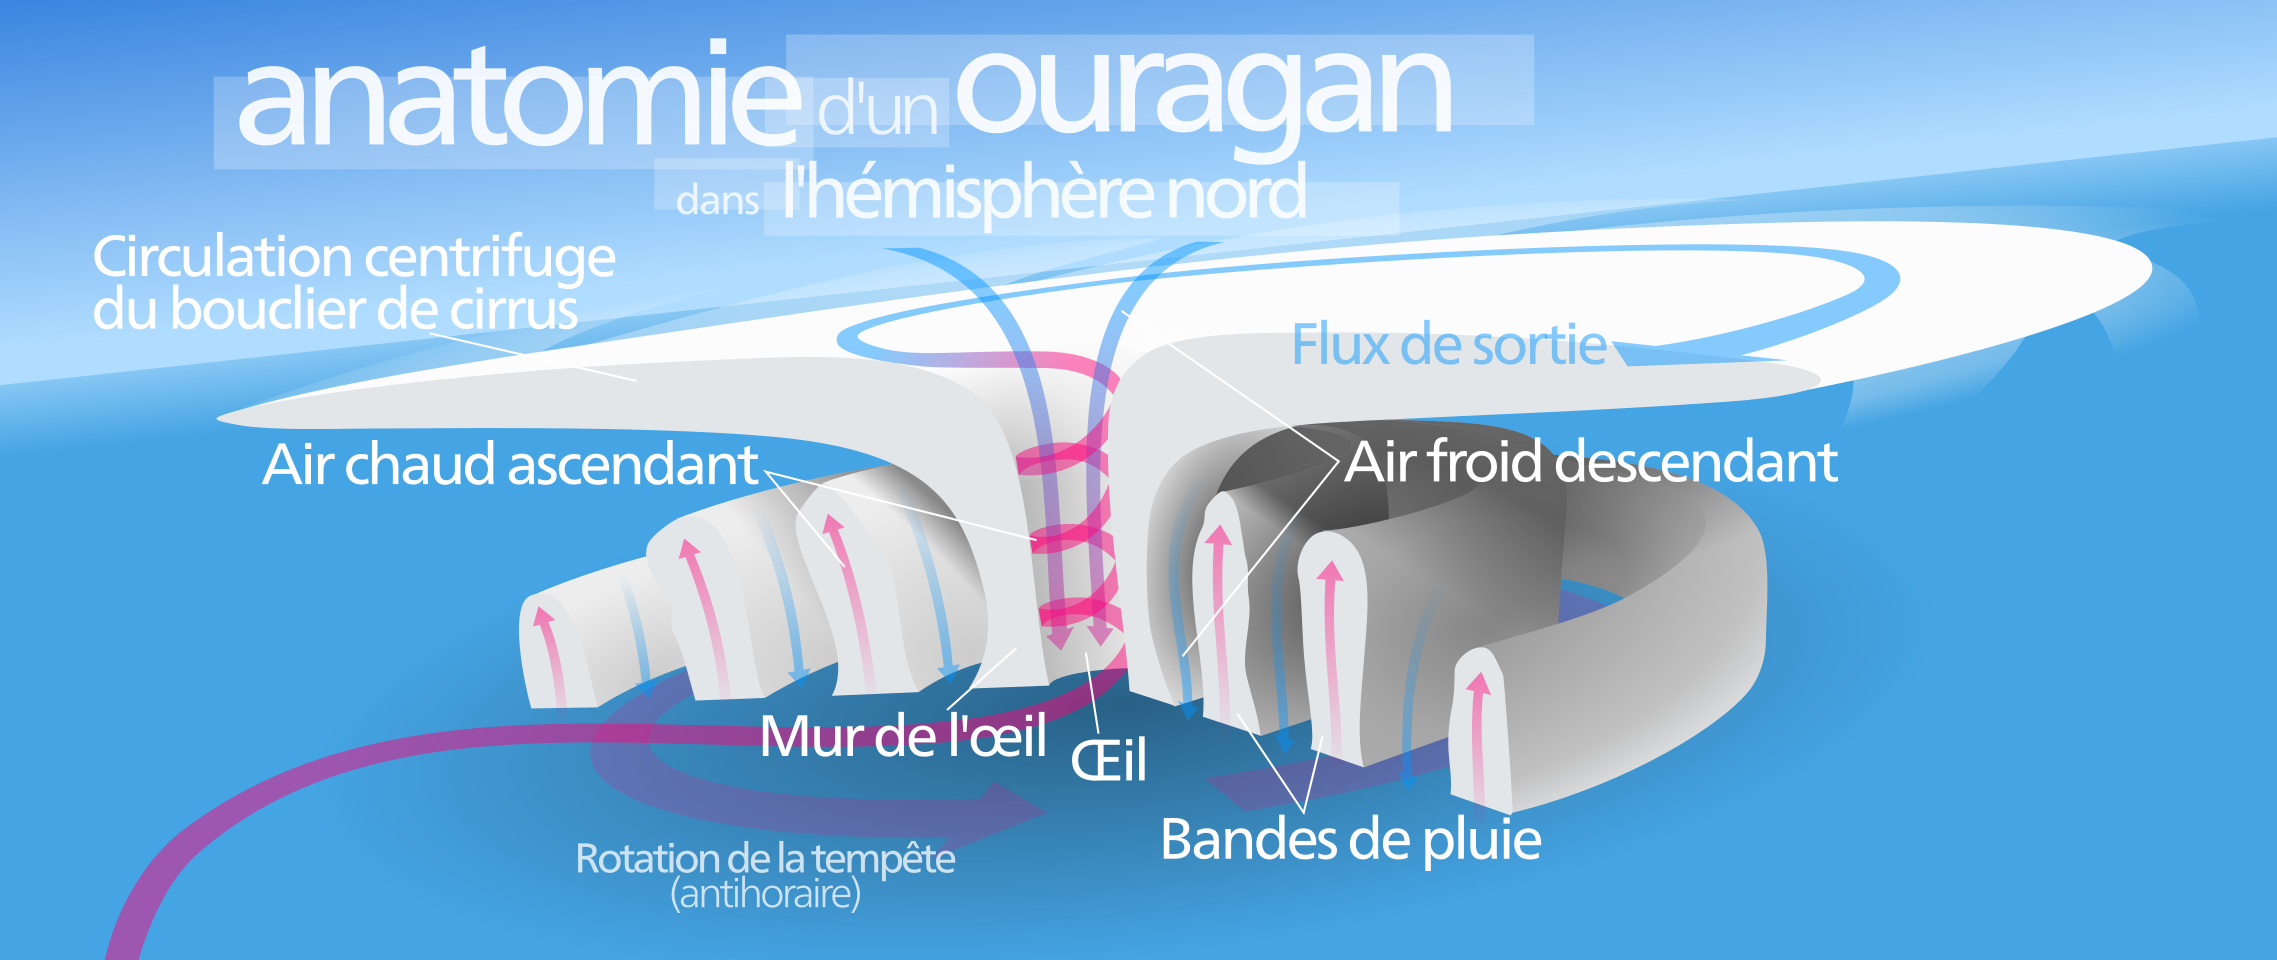
\includegraphics[width=0.9\textwidth]{Hurricane-fr.png}
    \caption{Diagramme en coupe d'un cyclone tropical, aussi appelé ouragan lorsqu'il survient dans l'océan Atlantique ou Nord-Est Pacifique --- By Kelvinsong -
    Own work, CC BY-SA 3.0, \url{https://commons.wikimedia.org/w/index.php?curid=23563610}}
    \label{fig:diagramme_TC}
\end{figure}
%
On dit que la perturbation dépressionnaire atteint le stade de cyclone tropical à proprement parler lorsque la vitesse du vent maximale à la surface et moyennée
sur une certaine période, variable selon les régions du monde, atteint le seuil de \ms{33}. En dessous de ce seuil, on parle soit de tempête tropicale si le
vent maximal est supérieur à \ms{17} ou bien de dépression tropicale si le vent maximal y est inférieur.

\subsection{Bassins d'activité et saisonnalité}\label{sec:bassins_saisons}

À l'échelle planétaire, il y a entre \numrange[range-phrase ={ et }]{82}{85} TC par an en moyenne selon les bases de données utilisées comme référence, et avec
un écart-type de \num{8} TC \parencite{schreck_impact_2014}. Cette activité globale est répartie sur un total de \num{6} grands bassins océaniques. Du point de
vue opérationnel, c'est à dire pour ce qui traite des aspects de surveillance et de prévision de l'activité cyclonique, ces bassins océaniques peuvent en
réalité être découpés en sous régions, dans lesquelles un centre météorologique régional spécialisé (CMRS, ou RSMC en anglais) ou un centre d'avertissements de
cyclones tropicaux (\textit{Tropical Cyclone Warning Centres}, TCWC) assure ces missions. Par exemple, l'océan Sud Indien est sous la tutelle conjointe, de part
et d'autre du 90\textsuperscript{ème} méridien Est, du CMRS de l'île de la Réunion (Météo-France) pour toute la partie Ouest, incluant le canal du Mozambique,
tandis que la surveillance de la partie Est est assurée par les TCWC de Perth, rattaché au Bureau of Meteorology (BoM) Australien, et de Jakarta. Néanmoins,
pour la régionalisation des analyses concernant l'activité cyclonique, nous favoriserons à travers ce document les grands bassins océaniques, et utiliserons des
définitions des domaines adaptées des recommandations de \cite{knutson_tropical_2020}, proposées dans un effort de standardisation afin de faciliter la
comparaison entre les études sur ce sujet. Ces bassins sont présentés sur la \cref{fig:bassins_TC}.
%
\begin{figure}[t]
    \centering
    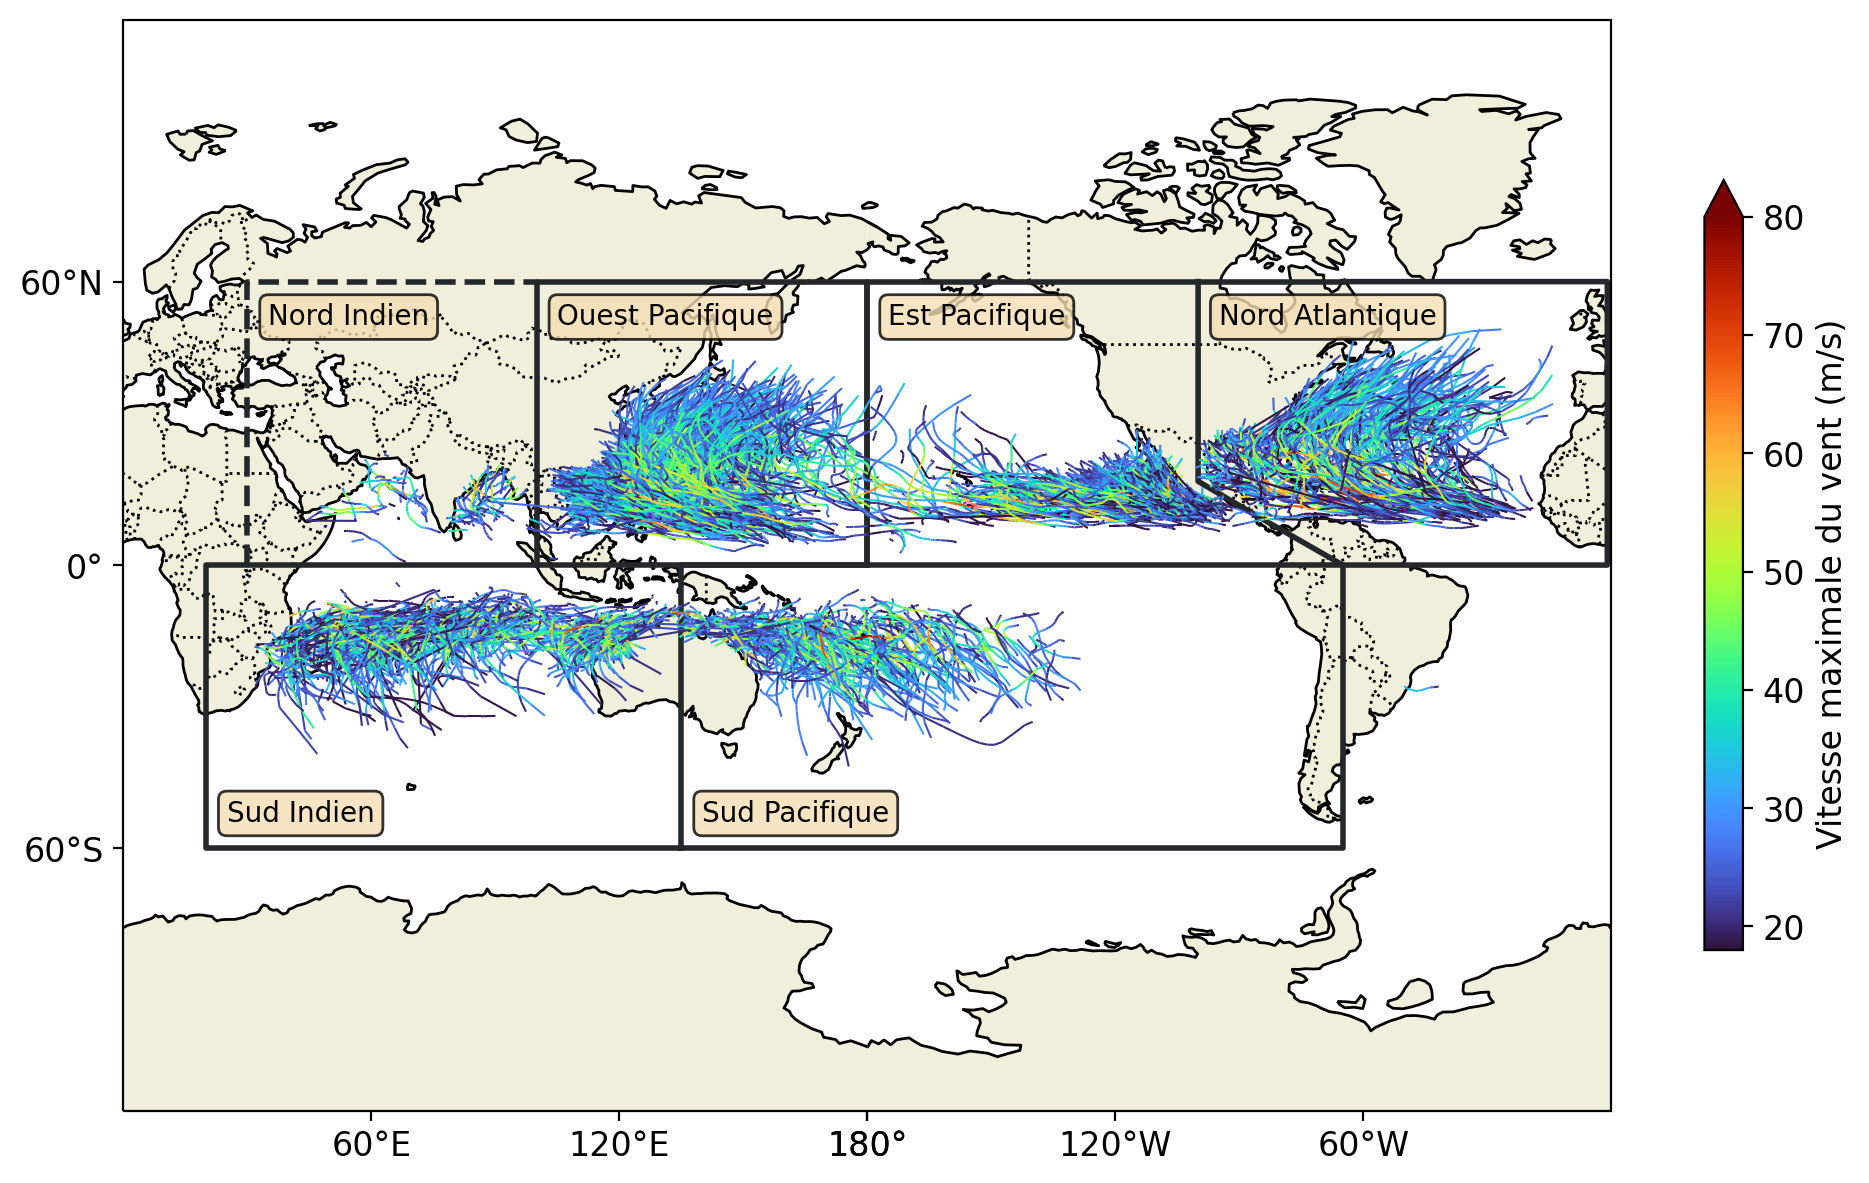
\includegraphics[width=0.9\textwidth]{Bassins_et_trajectoires.png}
    \caption{Bassins océaniques majeurs ainsi que les trajectoires des cyclones tropicaux observés entre 1981 et 2019, d'après la base de données
    \hbox{IBTrACS}. Les trajectoires sont colorées en fonction de l'intensité maximale des vents à chaque échéance. Les croix noires indiquent la première position observée de ces systèmes, assimilables aux cyclogénèses. Les définitions des bassins océaniques
    utilisées ici, et plus généralement dans l'ensemble de ce document, sont issues, à quelques modifications près, des recommandations de \hbox{\cite[documents
    supplémentaires]{knutson_tropical_2020}}.}
    \label{fig:bassins_TC}
\end{figure}
%
Le bassin océanique concentrant la plus grande activité est l'Ouest Pacifique (\textit{West Pacific}, WPac) avec environ \num{25} TC par an, ce qui représente
environ \SI{30}{\percent} de l'activité globale. Pour les autres régions de l'hémisphère nord : en deuxième place se trouve le bassin Est Pacifique (EPac) avec
une moyenne de \num{16.5} TC par an, suivi du bassin Nord Atlantique (NAtl) avec \num{12} TC par an et enfin le bassin Nord Indien (NInd) avec entre \num{4} et
\num{5} TC par an, bassin le moins actif du monde \parencite{gray_global_1968,lander_look_1998,schreck_impact_2014}. Ce dernier se distingue également par le
fait que le pays possèdent en réalité deux zones d'activité, de part et d'autre des côtes Indiennes : sur la Mer d'Arabie, à l'Ouest, et dans la Baie du
Bengale, à l'Est. Au total, l'hémisphère nord contient \SI{70}{\percent} de l'activité cyclonique globale. En ce qui concerne l'hémisphère sud, ses \num{24} TC
annuels en moyenne sont répartis entre l'océan indien (\textit{South Indian}, SInd) et l'océan pacifique (\textit{South Pacific}, SPac) avec une moyenne de
\num{14.6} TC pour le premier et \num{9.4} TC pour le second. Il arrive parfois que des systèmes cycloniques se forment dans le sud de l'océan atlantique, bien
que la région ne soit pas considérée comme bassin cyclonique actif et qu'elle ne possède pas de CMRS. Le cas le plus notable, et l'unique système ayant atteint
le seuil de vent nécessaire pour être classé comme cyclone tropical, est le cas du cyclone Catarina, en mars 2004 et ayant frappé les côtés Brésiliennes alors
qu'il était au plus fort de son intensité \parencite{mctaggart-cowan_analysis_2006}. La portion de trajectoire correspondant à la partie la plus intense de ce
cyclone est d'ailleurs visible sur la \cref{fig:bassins_TC}.
%
\begin{figure}[t]
    \centering
    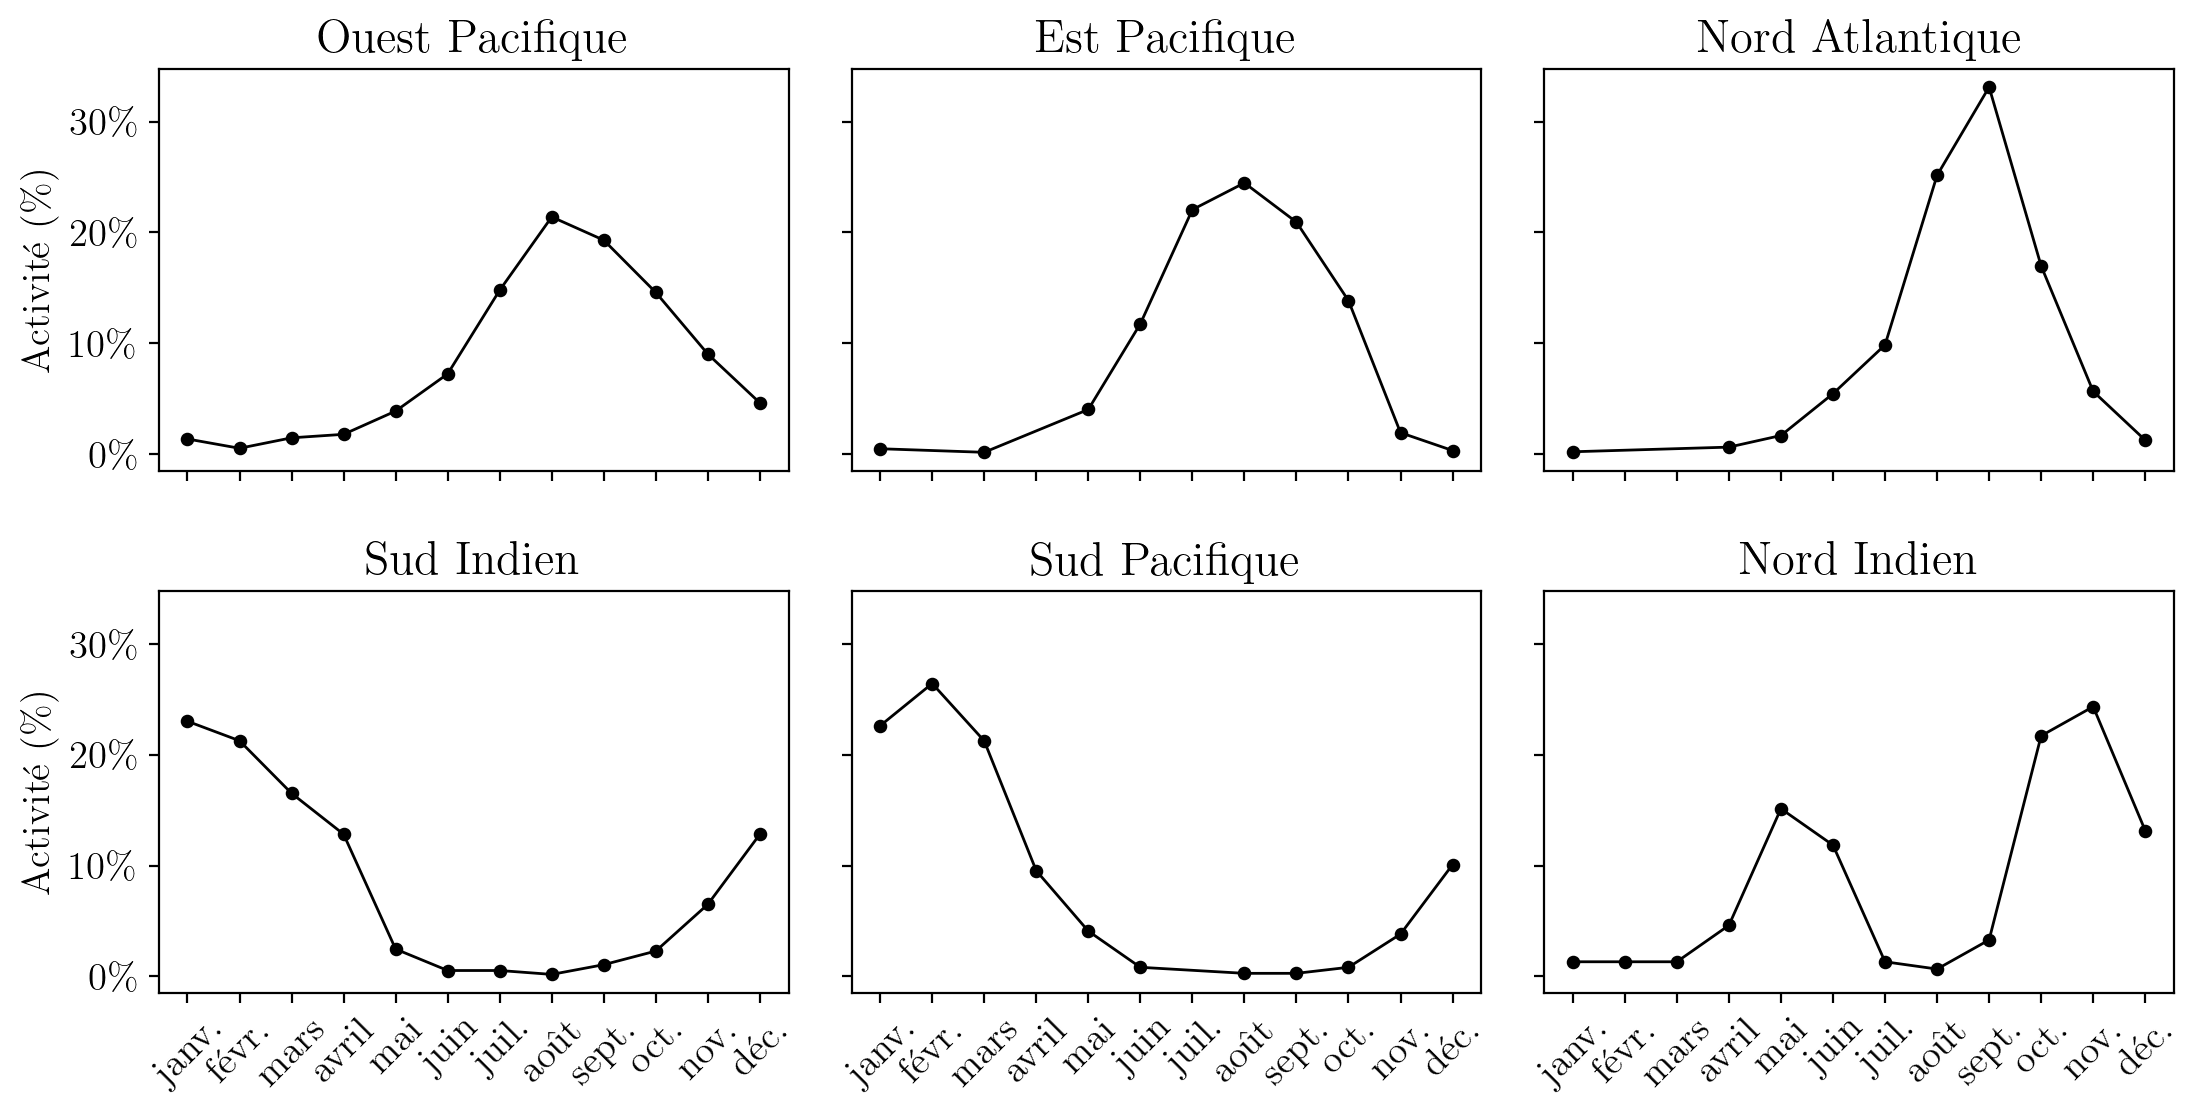
\includegraphics[width=\textwidth]{Saisons_TC.png}
    \caption{Saisonnalité de l'activité cyclonique tropicale dans les six bassins océaniques majeurs, normalisée pour chaque bassin et calculée à partir de la
    base de données IBTrACS entre 1981 et 2019 et en considérant pour chaque TC le mois de la première échéance où le stade de tempête tropicale est atteint.}
    \label{fig:saisons_TC}
\end{figure}
%
Les cyclones tropicaux surviennent principalement durant la saison chaude et avec un pic en fin de saison, avec plus ou moins d'étalement selon les régions,
avec pour exception notable le cas du bassin Nord Indien. Dans l'hémisphère sud, cela signifie que l'activité cyclonique est concentrée sur les mois de novembre
à avril, avec la plus grande partie située au delà de janvier, mais donc néanmoins répartie sur deux années calendaires. Pour cette raison, on considère dans
l'hémisphère sud que les saisons cycloniques courent de juillet de l'année précédente à juin de l'année courante, tandis qu'elle s'étend de janvier à décembre
dans l'hémisphère nord. Le cycle saisonnier des \num{6} bassins cycloniques majeurs est présenté sur la \cref{fig:saisons_TC}. Le bassin WPac présente la plus
grande dispersion, avec une activité comprise entre les mois de juin et de décembre, culminant au moins d'août. Pour l'EPac, la saison est un peu plus courte
puisque, si elle commence également autour de juin, le mois de novembre ne voit quant à lui quasiment aucune activité. Le bassin NAtl présente une activité
encore plus recentrée avec un pic en septembre qui concentre un tiers de l'activité du bassin. Le bassin SInd voit sa saison débuter en novembre avec un pic en
janvier, tandis que le SPac démarre un mois plus tard, en décembre, et présente un pic d'activité en février avec \SI{26}{\percent} de son activité qui est
concentrée sur ce mois. Enfin, le bassin NInd se distingue ici une fois de plus puisque son cycle annuel fait apparaître deux périodes d'activité. La première,
mineure, prend place de avril à juillet, tandis que la seconde, plus importante, a lieu de septembre à janvier. Cette coupure dans le cycle annuel s'explique
par le phénomène de mousson indienne, qui a lieu durant l'été, et qui apporte du cisaillement vertical dans l'atmosphère, élément défavorable à la cyclogénèse
\parencite{gray_global_1968}, comme développé dans la \cref{sec:conditions_cyclogenese}.

\subsection{Risques associés et enjeux}\label{sec:risques}

Les cyclones tropicaux constituent les événements météorologiques les plus extrêmes, les plus destructeurs et aussi les plus dangereux pour les populations.
D'après l'étude de \cite{doocy_human_2013}, le nombre médian de victimes par TC s'élève à \num{14} vies (\num{430} en moyenne), pour un bilan humain total
estimé entre les années 1980 et 2009 à \num{412644} morts et \num{290654} blessés. Les deux tiers de ce nombre sont attribués à seulement deux évènements : Le
cyclone Gorky de 1991 ayant fait \num{138866} victimes au Bangladesh, et le cyclone Nargis en 2008, en Birmanie, avec \num{138366} victimes. Outre les morts, le
nombre total de personnes affectées d'une façon ou d'une autre par les TC est estimé à plus de \num{466} millions, ce qui inclut \num{20} millions de personnes
qui se sont retrouvées sans abri \parencite{doocy_human_2013}. Ainsi, la région de l'Asie du Sud-est, telle que définie par l'Organisation Mondiale de la Santé,
concentre \SI{80}{\percent} des décès causés par les cyclones tropicaux, et \SI{53}{\percent} de la population affectée, tandis qu'elle ne concentre que
\SI{9}{\percent} des évènements impactants, ce qui montre alors que les plus forts impacts sont causés par quelques évènements extrêmes.

Pour ce qui est du coût des dégâts matériels associés aux TC, ils sont difficiles à estimer à l'échelle globale car ils n'ont étés rapportés que dans
\SI{15.4}{\percent} des cas, toujours d'après \cite{doocy_human_2013}. Ces coûts sont néanmoins d'autant plus importants que les pays concernés sont riches et
dotés d'infrastructures coûteuses. Le Centre National d'Information sur l'Environnement (NCEI) de l'Agence Américaine d'Observation Océanique et Atmosphérique
(NOAA) recense tous les évènements météorologiques extrêmes impactant les États-Unis dont les coûts dépassent le seuil de \num{1}~milliard de dollars. Ainsi,
entre 1980 et 2020, les dégâts causés par les cyclones tropicaux sont évalués, en tenant compte de l'inflation, à \num{1145.3}~milliards de dollars, ce qui
concentre \SI{52.3}{\percent} du coût total causé par l'ensemble des extrêmes météorologiques considérés ---~loin devant la deuxième plus importante cause de
dégâts matériels, à savoir les fortes tempêtes, qui concentrent \SI{15}{\percent} des coûts totaux~--- et ce qui représente un coût moyen de \num{21.6}~milliard
de dollars par évènement \parencite{smith_billiondollar_2020}.

Les risques associés aux TC sont nombreux et divers : vents extrêmes, fortes précipitations et inondations, orages, tornades et glissements de terrain. Mais le
plus grand risque provient des ondes de marées. Sous l'effet conjugué des vents et de la pression centrale du cyclone, le niveau de la mer augmente fortement et
rapidement, provoquant des inondations pouvant s'étendre sur plusieurs dizaines de kilomètres. Les ondes de marées sont le danger principal associé aux TC et
aussi la première cause de mortalité durant ces évènements \parencite{needham_review_2015}. Si chacun de ces risques peut, lorsque pris individuellement, causer
des pertes considérables, matérielles comme immatérielles, le danger est d'autant plus grand lorsque ces aléas surviennent simultanément et interagissent entre
eux, avec des impacts pouvant perdurer longtemps après le passage du cyclone. En effet, suite au passage d'un cyclone tropical, il n'est pas rare de voir
l'émergence de maladies infectieuses, en particulier dans les pays en voie de développement \parencite{shultz_epidemiology_2005}. Cette émergence se voit en
effet favorisée, entre autres, par la perturbation des infrastructures de santé publique ---~incluant les hôpitaux et les centres de soins, mais également les
réseaux de distribution en eau potable~--- mais aussi par les regroupements des populations dans des refuges surpeuplés, et plus généralement par une plus
grande exposition de ces derniers à l'environnement suite aux dommages causés aux habitations. Il en ressort donc que les dégâts matériels et économiques causés
par les cyclones tropicaux peuvent également avoir un coût en vies humaines.

Plus un cyclone tropical est large et intense, plus les risques sont accrus. Bien qu'il soit difficile de déterminer précisément la relation liant l'intensité
d'un cyclone et les dégâts associés, il est néanmoins admis que le potentiel de destruction d'un cyclone dépend au moins de l'intensité de ses vents. Une
métrique classiquement utilisée pour quantifier l'activité cyclonique sur une saison donnée est bien représentée par l'énergie cinétique cumulée des cyclones au
cours de celle-ci. Pour la calculer, on fait la somme des vents maximums soutenus, élevés au carré, avec une période de six heures, sur l'ensemble des systèmes
de la saison lorsqu'ils dépassent au moins le stade de tempête tropicale~--- métrique appelée l'énergie cumulative des cyclones tropicaux (\textit{Accumulated
Cyclone Energy}, ACE, \cite{bell_climate_2000}). Si d'autres métriques sont parfois utilisées et jugées plus pertinentes pour évaluer le potentiel destructeur
d'un TC, elles restent toutefois basées sur la vitesse du vent \parencite{powell_tropical_2007}. En supposant que le risque cyclonique demeure constant
dans un climat plus chaud et que les pays concernés par ce risque continuent à se développer, alors les dégâts économiques ne peuvent qu'augmenter. Sous cette
hypothèse de stationnarité, les travaux de \cite{ye_dependence_2020} suggèrent qu'un doublement de la valeur des actifs exposés à ce risque en Chine pourrait
engendrer une hausse de \SI{80}{\percent} des dégâts économiques induits par les TC. Or, rien ne permet d'affirmer la validité de cette hypothèse, étant données
les incertitudes associées aux projections futures de l'activité cyclonique tropicale (voir \cref{sec:projections_futures}). Par conséquent, l'évolution de
l'activité cyclonique dans un contexte de réchauffement global, en particulier pour ce qui concerne les questions d'intensité et de fréquence des TC, constitue
un enjeu de première importance.

%----------------------------------------------------------------------------------------------------------------------
\section{Ingrédients de la cyclogénèse}
  
\subsection{Conditions de formation}\label{sec:conditions_cyclogenese}

On appelle \textquote{cyclogénèse} le processus par lequel un cyclone tropical se développe et s'intensifie. Bien que les mécanismes précis permettant
d'expliquer ce processus ne soient pas encore bien compris, malgré des décennies d'efforts consacrés à cette question \parencite{yanai_formation_1964, gray_global_1968, 
montgomery_tropical_1993, gray_formation_1998, tory_tropical_2010}, il existe néanmoins un consensus quant aux facteurs qui y sont favorables. Les travaux de
\cite{gray_global_1968}, complétés dans \cite{gray_tropical_1975}, constituent, à partir des observations disponibles à l'époque, une étude globale sur
l'origine des cyclones tropicaux et font référence en la matière. Six facteurs sont ainsi identifiés et brièvement présentés ci-dessous.

\subsubsection*{Vorticité relative en basses couches}

Les cyclones tropicaux se forment toujours à partir de perturbations atmosphériques préexistantes. Ce sont souvent des petits systèmes dépressionnaires
provenant de la zone de convergence intertropicale (ZCIT) \parencite{gray_global_1968}, ou encore des ondes d'est tropicales, comme dans le cas de l'océan
Atlantique où ces ondes peuvent jouer le rôle de précurseurs \parencite{thorncroft_african_2001,patricola_response_2018}. Les ondes d'est africaines en provenance
de la région du Sahel sont à l'origine de plus de \prct{90} des cyclones majeurs dans l'Atlantique nord \parencite{landsea_strong_1992}. Ces perturbations apportent
une vorticité initiale, ou tourbillon, qui, par convergence frictionnelle, apporte de la vapeur d'eau provenant de la mer vers le cœur du système, au niveau de la
couche limite atmosphérique. Cette vapeur est entrainée en altitude par mouvement convectif, puis condensée, libérant de ce fait de la chaleur latente en haute
troposphère, contribuant ainsi à entretenir le fonctionnement du cyclone. Ce mécanisme constitue la source principale d'énergie des cyclones tropicaux
\parencite{emanuel_dependence_1987}.

\subsubsection*{Rotation de la Terre}

La rotation de la Terre induit, du point de vue d'un observateur appartenant au même référentiel, une force sur tous les objets se déplaçant à la surface de la
planète et appelée force de Coriolis. Cette force, qualifiée d'inertielle ou de fictionnelle, en ce sens qu'elle n'est le résultat que du fait que le
référentiel d'observation est non inertiel. Dans le cas des cyclones tropicaux, la force de Coriolis cause la formation de deux circulations secondaires de partet d'autre du cyclone : Une circulation cyclonique à l'ouest et anticyclonique à l'est. La résultante de ces deux circulations secondaires tend à déplacer le cyclone vers le nord-ouest dans l'hémisphère nord, et vers le sud-ouest dans l'hémisphère sud.

Mais outre l'effet sur leur trajectoires, la rotation de la Terre joue également un rôle primordial dans la circulation cyclonique, puisque c'est cette force qui
est à l'origine même du mouvement de rotation dans la circulation cyclonique. Cette force varie avec le sinus de la latitude et est donc nulle à l'équateur. À
proximité de l'équateur, la force de Coriolis est dirigé verticalement  et sa composante horizontale est donc négligeable et les vents de la couche limite atmosphérique ne sauraient se maintenir au delà de quelques
mètres par secondes \parencite{gray_tropical_1975}. La force de Coriolis permet au vortex d'atteindre l'équilibre du vent gradient, mentionné dans la
\cref{sec:quest_ce_qu_un_cyclone} et donc de se développer jusqu'à devenir un cyclone tropical. Par conséquent, la cyclogénèse ne peut pas se produire à
l'équateur, et les observations historiques indiquent qu'une distance à l'équateur de \num{4}~à~\ang{5} est requise pour qu'un cyclone tropical puisse se
développer \parencite{gray_global_1968}.

\subsubsection*{Faible cisaillement vertical du vent}

Le cisaillement du vent, ou plus précisément ici, le cisaillement vertical du vent horizontal, exprime la manière dont le vent horizontal varie avec l'altitude,
en intensité comme en direction. Dans le cas des cyclones tropicaux, on le mesure (ou le calcule) sur toute la hauteur de la troposphère, c'est à dire entre la
tropopause à \hPa{200} et la basse troposphère, typiquement à \hPa{850}. Un cisaillement vertical important cause l'advection de la chaleur libérée par la condensation des cumulonimbus dans les hautes couches dans une direction différente par rapport à la chaleur libérée dans les basses couches, si bien que que la capacité du système à accumuler de la chaleur en son cœur s'en voit fortement limitée \parencite{gray_global_1968}.  Le cisaillement vertical apparaît alors comme très défavorable à la cyclogénèse.

\subsubsection*{Température de surface de la mer}

Un cyclone tropical consomme environ \SI{15}{\mega\joule} par jour de chaleur sensible et latente extraite de la surface océanique
\parencite{gray_tropical_1975}. De plus, la circulation cyclonique produit un mélange des eaux océaniques sous-jacentes et donc un refroidissement des SST par remontée des eaux situées sous la thermocline. Pour ces
raisons, la cyclogénèse nécessite non seulement que la température de surface océanique (\textit{sea surface temperature}, SST) dépasse un certain seuil
---~évalué empiriquement à \SI{26}{\degreeCelsius}\footnote{Le seuil de \SI{26}{\degreeCelsius} a été déterminé avec les observations historiques et est valable pour le climat présent. Il est cependant susceptible de changer avec le réchauffement climatique, sinon quoi les scénarios futurs indiqueraient une explosion du nombre de cyclone, ce qui n'est pas le cas. Voir aussi \cref{sec:projections_futures}.}, sinon quoi la flottabilité n'est pas suffisante pour assurer la convection \parencite{palmen_formation_1948}~--- mais
également que cette température soit atteinte sur au moins \m{60} de profondeur d'eau \parencite{leipper_observed_1967,perlboth_hurricane_1967}. En effet, si la couche de mélange océanique n'est pas suffisamment profonde, alors la SST ne sera plus à même d'alimenter le cyclone. Ce besoin
important en chaleur a généralement pour conséquence l'affaiblissement rapide du TC mature lorsqu'il atteint les terres.

\subsubsection*{Humidité relative et instabilité atmosphérique}

Ces deux derniers facteurs que sont l'humidité relative en moyenne troposphère, c'est à dire autour de \hPa{600}, et la notion de stabilité atmosphérique, sont,
dans le cadre de la cyclogénèse, étroitement liés. La stabilité de l'atmosphère, à fortiori lorsqu'elle est chargée en vapeur d'eau, dépend du gradient vertical
de température potentielle équivalente, notée $\theta_e$ et définie comme la température que la parcelle d'air atteindrait si tout son contenu en vapeur d'eau
venait à condenser et qu'elle était ramenée au niveau du sol de manière adiabatique. Le processus de convection des cumulonimbus, à l'origine de la formation
d'un cyclone tropical, nécessite en effet une forte diminution de $\theta_e$ entre la couche limite atmosphérique et la moyenne troposphère, c'est à dire une
atmosphère instable. Par ailleurs, la convection profonde est favorisée par une atmosphère à haute humidité relative en moyenne troposphère, car à température
égale, une parcelle d'air humide possède une plus grande flottabilité qu'une parcelle d'air sec. Enfin, toujours d'après \cite{gray_tropical_1975}, une humidité relative élevée en haute troposphère favorise l'efficacité des pluies, tandis qu'une plus grande fraction de l'eau precipitée est ré-évaporée avant d'atteindre le sol dans une atmosphère sèche. La ré-évaporation de l'eau contribue à refroidir la moyenne troposphère, ce qui est défavorable à la cyclogénèse, et donc une atmopshère humide est quant à elle favorable.

\subsubsection*{Climatologies}\label{sec:climato_ingredients}

La \cref{fig:clim_ingredients} présente les climatologies saisonnières de quatre des éléments favorables à la cyclogénèse que sont la vorticité absolue à
\hPa{850}, notée $\zeta_{\text{\hPa{850}}}$; l'humidité relative à \hPa{600}, $\text{RH}_{\text{\hPa{600}}}$ ; l'inverse du cisaillement vertical du vent
horizontal entre \hPa{200} et \hPa{850}, noté $1/S_z$ et enfin la SST relative aux tropiques, définie comme la différence entre la SST et la SST moyenne entre \ang{20}S et \ang{20}N. Ces champs sont issus de la réanalyse ERA5 du Centre européen pour
les prévisions météorologiques à moyen terme (CEPMMT, ou juste CEP ; en anglais \textit{European Centre for Medium-Range Weather Forecasts}, ECMWF)
\parencite{hersbach_era5_2020}, laquelle est décrite plus en détails dans la \cref{sec:eval_tracker_ERA5}. Notons que la vorticité absolue $\zeta$ à \hPa{850} intègre
déjà le paramètre de Coriolis, noté $f$, auquel le module de la force éponyme est proportionnel, puisque la vorticité absolue est définie comme
%
\begin{equation*}
    \zeta = \zeta_R + \underbrace{2 \Omega \sin \phi}_{f}
\end{equation*}
%
où $\zeta_R$ est la vorticité relative, définie comme le rotationel du vent tel que mesuré dans le référentiel de la Terre, $\Omega$ la période de
rotation de la Terre et $\phi$ la latitude. L'inverse du cisaillement vertical est pris de telle façon à ce que des valeurs élevées indiquent des régions
favorables à la cyclogénèse et la SST relative permet ici de faire apparaître les variations locales plus nettement.

\begin{figure}[tp]
    \centering
    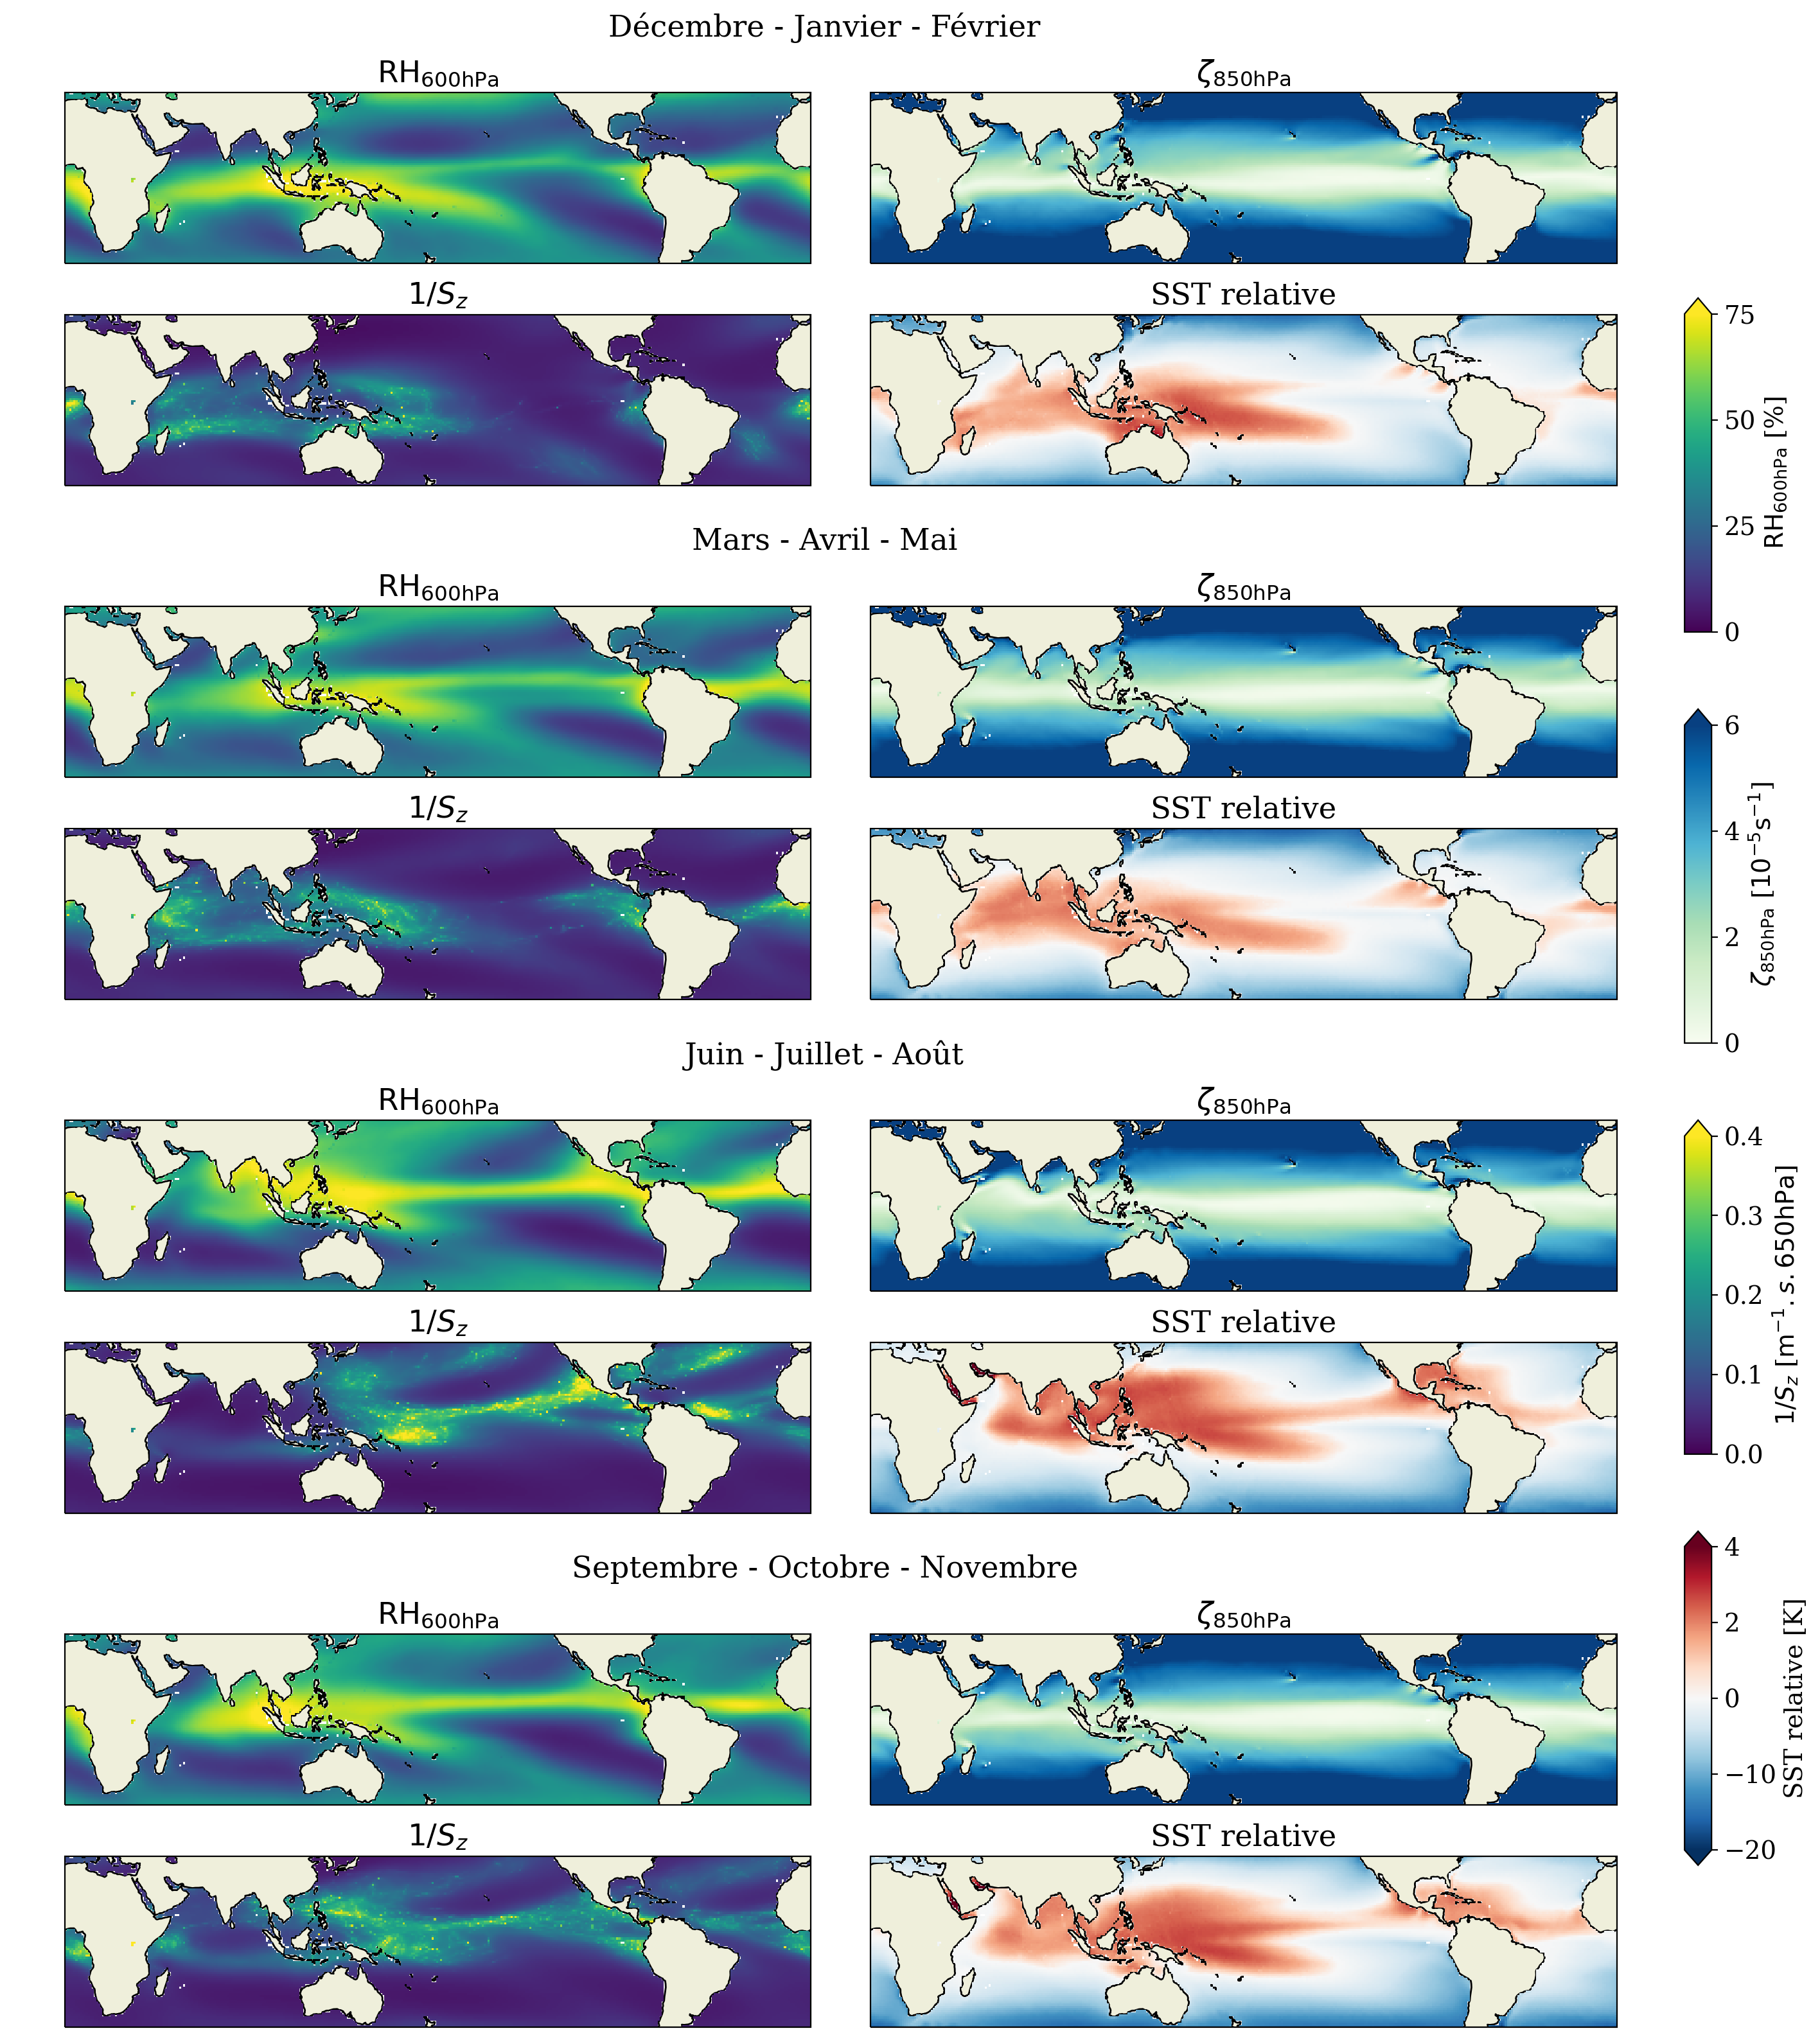
\includegraphics[width=\textwidth]{clim_saison_hurel_rotu_shear_sst.png}
    \caption{Climatologies saisonnières de l'humidité relative à \hPa{600}, de la vorticité absolue à \hPa{850}, de l'inverse du cisaillement vertical entre
    \hPa{200} et \hPa{850} et de la SST relative à la température moyenne le long de la ceinture tropicale, entre \ang{20}S et \ang{20}N, calculées à partir de
    moyennes mensuelles de la réanalyse ERA5 entre 1979 et 2020 et avec une résolution horizontale de \ang{1}.}
    \label{fig:clim_ingredients}
\end{figure}

Au premier abord, la SST apparaît comme un des facteurs prédominants dans la répartition spatiale et temporelle de l'activité cyclonique, puisqu'on retrouve sur
ces cartes de SST relatives la répartition géographique des cyclogénèses présentées sur la \cref{fig:bassins_TC} (. L'humidité
relative et le cisaillement laissent également apparaître cette répartition spatiale, avec toutefois quelques nuances supplémentaires, notamment dans les
régions extra tropicales. La climatologie de la vorticité est en revanche moins lisible mais présente localement des variations saisonnières dans l'étendue
méridionale du bandeau tropical. Par ailleurs, les variations saisonnières de ces quatre paramètres coïncident également avec l'activité mensuelle présentée sur
la \cref{fig:saisons_TC}. Cet accord est particulièrement visible sur les tracés de SST, avec des températures relatives de surface des océans très prononcées
dans l'Atlantique nord et l'Indo-Pacifique nord pendant les saisons Juin~-~Juillet~-~Août (JJA) ainsi que
Septembre~-~Octobre~-~Novembre (SON). Cette configuration spatiale s'inverse dans l'Indo-Pacifique sud durant les saisons Décembre~-~Janvier~-~Février (DJF) et
Mars~-~Avril~-~Mai (MAM), où la partie sud présente une anomalie spatiale plus forte. Le bassin NInd durant la saison JJA constitue un cas particulier, déjà
évoqué précédemment (c.f \cref{sec:bassins_saisons}), puisque l'humidité relative, la vorticité et la SST y sont toutes trois élevées, tandis que l'activité
cyclonique y est quasi nulle (c.f \cref{fig:saisons_TC}). En effet, cette saison correspond à la mousson d'été en Inde, laquelle apporte du fort cisaillement
vertical, si bien que $1/S_z$ avoisine zéro. Cela illustre à nouveau le rôle essentiel du cisaillement dans le processus de cyclogénèse et
souligne le fait que c'est bien la combinaison de tous les ingrédients qui mène à la cyclogénèse.

En première approche, il est possible d'estimer la climatologie spatiale et saisonnière des zones où les conditions favorables sont réunies en prenant
simplement le produit des quatre variables présentées sur la \cref{fig:clim_ingredients}. C'est ce que montre la \cref{fig:produit_ingredients}, avec en
superposition les premières occurences des trajectoires des cyclones tropicaux observés entre 1981 et 2019, celles là mêmes qui sont présentées sur la
\cref{fig:bassins_TC}. Ces points peuvent être assimilés aux cyclogénèses, malgré l'incertitude qui peut exister sur leur localisation exacte. Ce produit est ici défini comme suit :
%
\begin{equation*}
    \text{RH}_{\hPa{600}} \times \zeta_{\hPa{850}} \times \frac{1}{S_z} \times \text{SST} \quad \text{[$10^{-5}$ K m$^{-1}$ \hPa{650}}]
\end{equation*}
%
\begin{figure}[tbp]
    \centering
    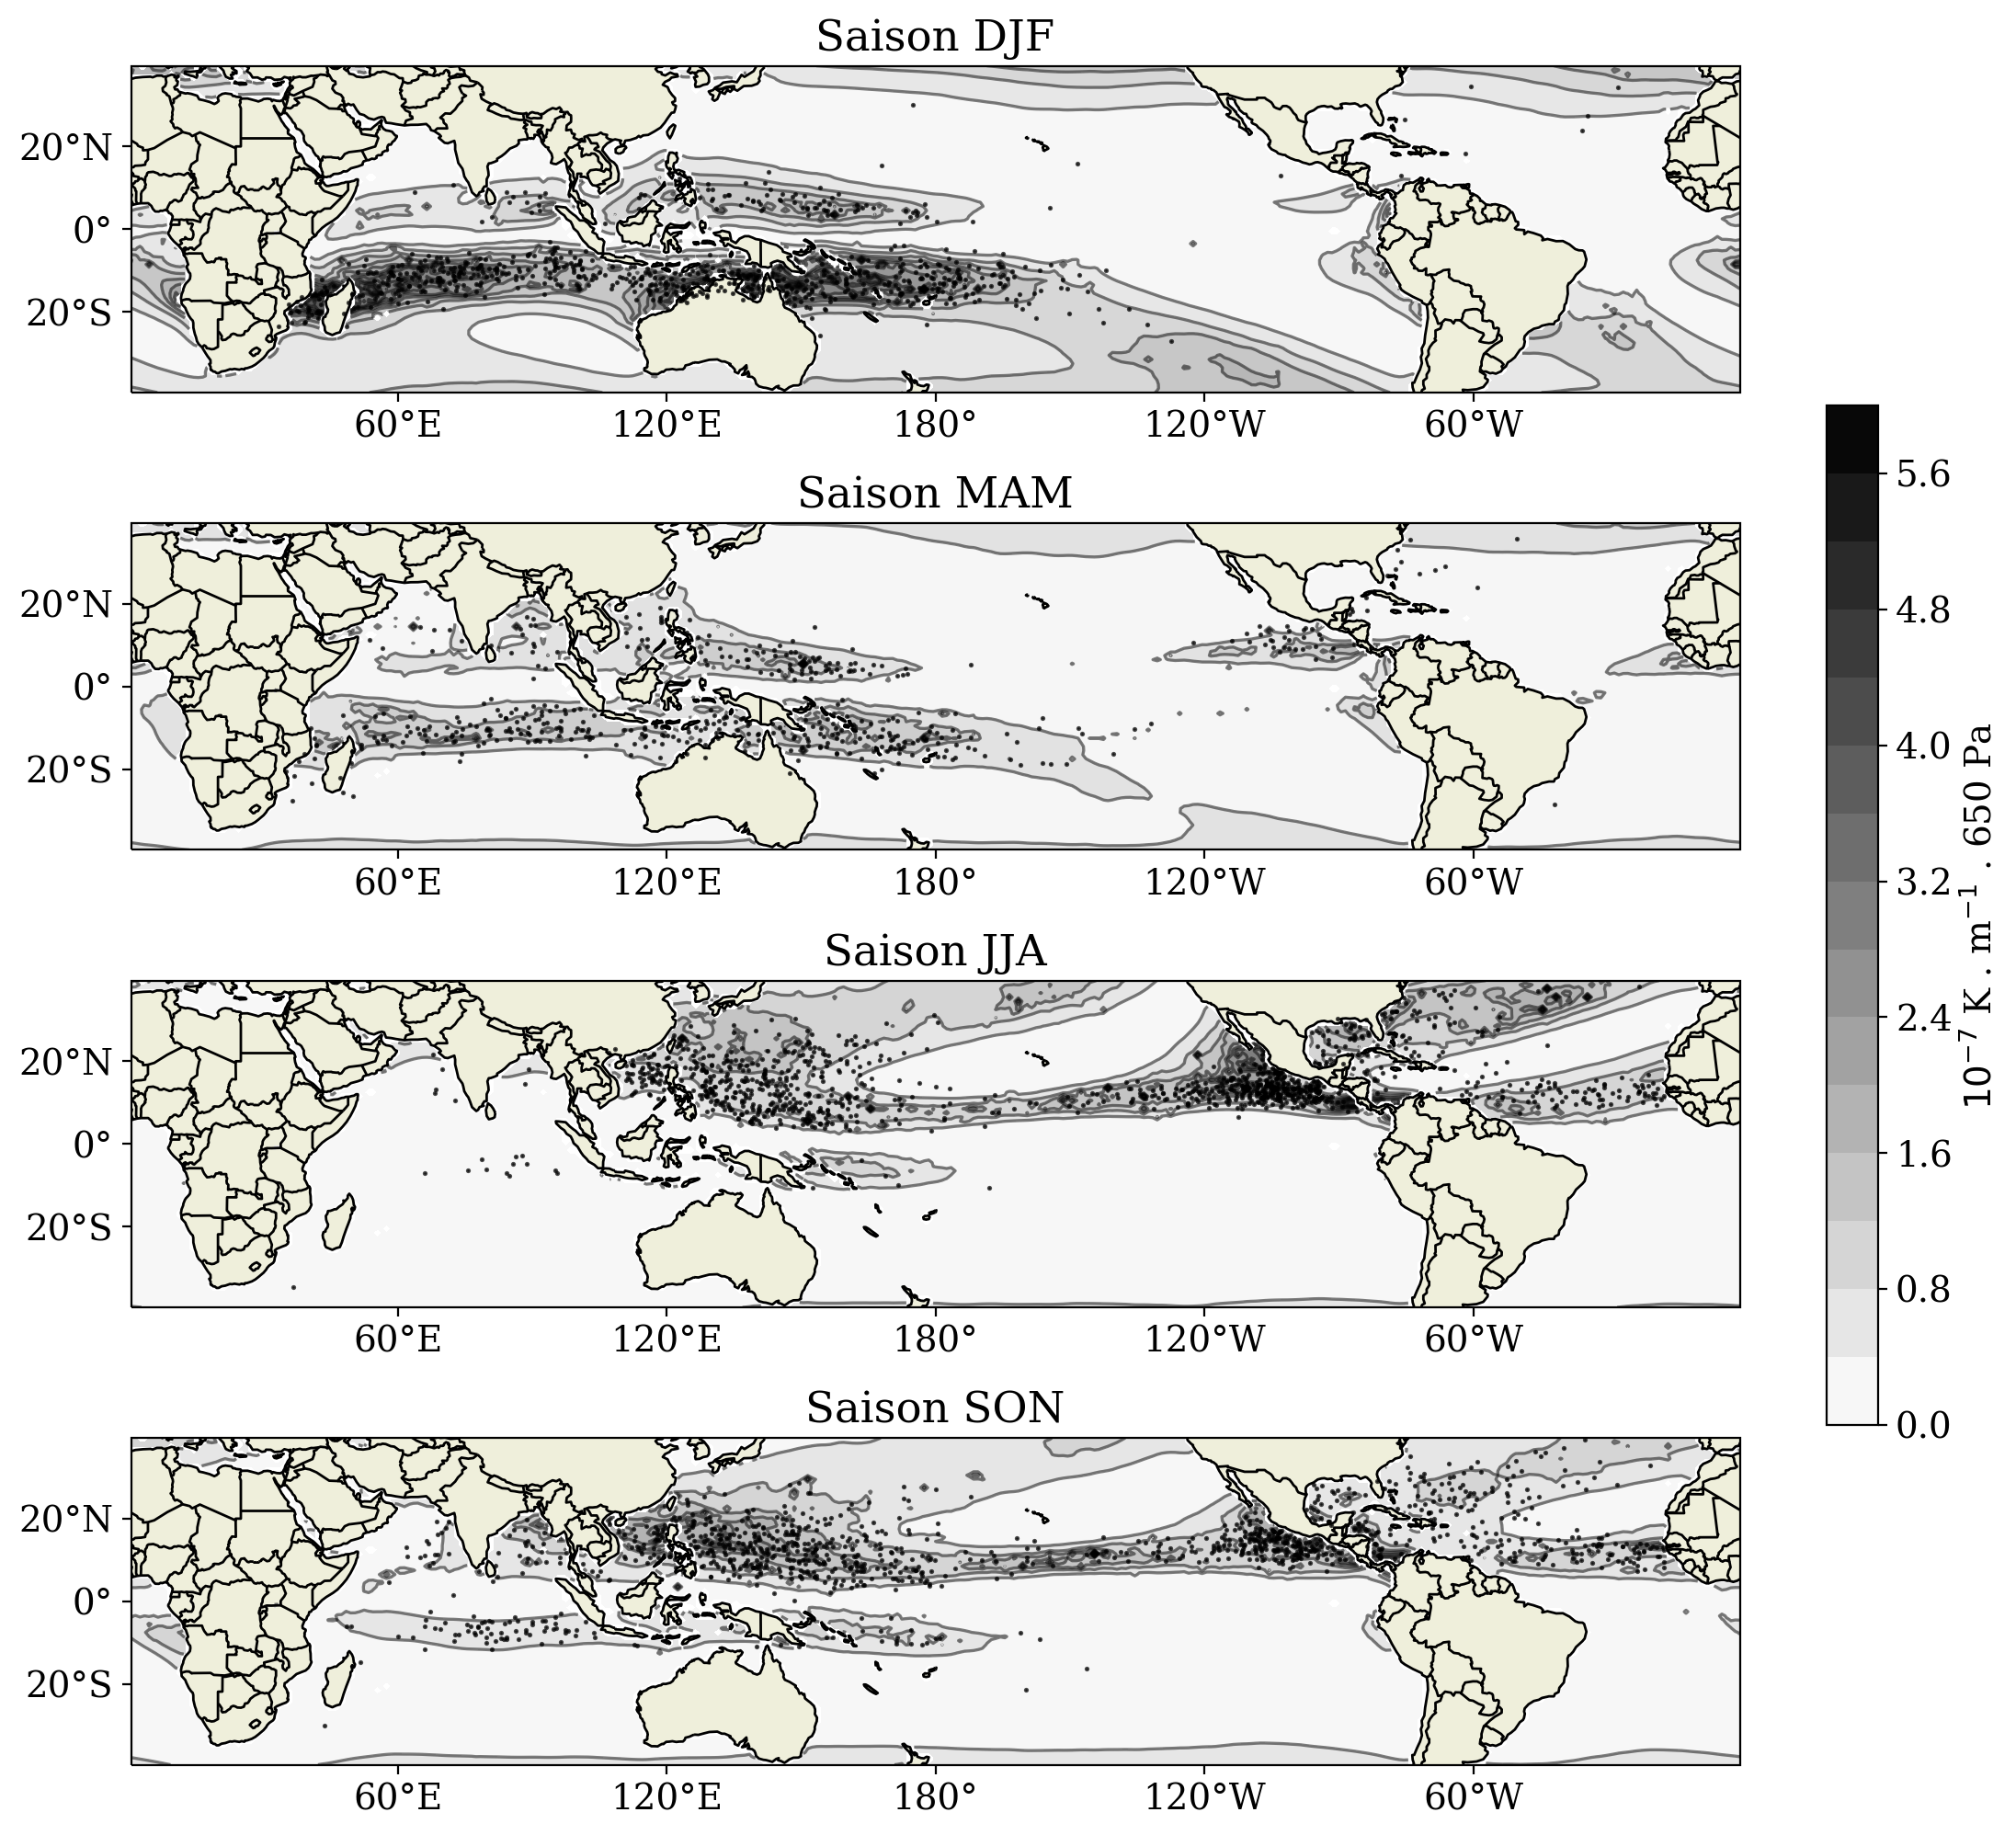
\includegraphics[width=1\textwidth]{clim_saison_produit_ingredients_et_ibtracs.png}
    \caption{Climatologies saisonnières du produit des quatre variables présentées sur la \cref{fig:clim_ingredients}, où la SST est ici simplement la
    température de surface de l'océan, sans considérer l'écart aux tropiques. Sont représentés par des points noirs pour chaque saison les premières
    observations des trajectoires présentées sur la \cref{fig:bassins_TC}.}
    \label{fig:produit_ingredients}
\end{figure}
%
Cette figure montre un excellent accord entre le produit des quatre variables et la cyclogénèse observée, aussi bien dans la répartition géographique que temporelle. Quelques points de discorde demeurent cependant, avec une extension vers les moyennes latitudes des zones indiquées comme favorables par le produit des quatre variables, tandis que les cyclogénèses y sont quasiment inexsitantes. On distingue dans ces zones l'empreinte conjointe de l'humidité relative et du cisaillement, lesquelles présentent la même structure sur la \cref{fig:clim_ingredients}. Dans la ceinture tropicale et sub-tropicale, la correspondance entre le produit des paramètres et l'activité observée demeure cependant remarquable. Ce constat selon lequel la fréquence d'occurrence des cyclones tropicaux en un lieu donné puisse être proportionnelle à une combinaison de variables de grande échelle, découverte attribuée à \cite{gray_tropical_1975}, est à l'origine de ce qui sera nommé par la suite les indices de cyclogénèse, et qui seront abordés plus en détails dans la \cref{sec:intro_indices}, puis dans le \cref{chap:chapitre_3}.

% \subsection{Modèles conceptuels de fonctionnement}
% 
% \subsubsection{CISK}
% 
% \cite{charney_growth_1964,ooyama_dynamical_1964,ooyama_numerical_1969}
% 
% \subsubsection{WISHE}
% 
% \cite{emanuel_airsea_1986,emanuel_largescale_1994}

%----------------------------------------------------------------------------------------------------------------------
\section{Cyclones tropicaux et changement climatique}

\subsection{Bases de données observationnelles et tendances historiques}\label{sec:observations}

Un pré-requis pour pouvoir traiter de changement climatique, quelque soit l'objet d'étude, est de disposer de données observationnelles le plus fiables
possibles, et sur la plus longue période possible. Or, les réseaux d'observation s'étendent et se densifient, les instruments se perfectionnent avec le temps,
de nouvelles techniques de mesure émergent et donc les incertitudes associées aux observations tendent à diminuer, ce qui donne alors lieu à de fortes
hétérogénéités et ruptures temporelles dans la qualité des données. L'observation des cyclones tropicaux ne fait pas exception à cette règle. Les cyclones étant
des phénomènes prenant place sur mer, les premiers relevés météorologiques de cyclones tropicaux étaient réalisés par les marins et consignés dans leurs journaux
de bords \parencite{knapp_international_2010}. Avec le temps, et étant donné le fort potentiel d'impact de ces systèmes, les sources d'observations se sont
multipliées et diversifiées, de manière très inégale selon les régions. Les États-Unis déploient par exemple des avions de reconnaissance dédiés à la recherche et
à l'observation des cyclones tropicaux au large des côtes atlantiques depuis \num{1946}, bassin océanique qui est encore à ce jour le seul à bénéficier de ce type
d'observations de manière régulière. D'autres sources d'observations incluent notamment les stations météorologiques terrestres, bouées instrumentées, radars et
enfin radio sondages, ces derniers pouvant être réalisés par largage aérien directement dans le cyclone. Néanmoins, la véritable rupture technologique a lieu
avec l'ère satellitaire, réellement entérinée à la fin des années 70. L'observation par satellite permet d'une part de détecter la quasi totalité des cyclones,
mais aussi d'estimer systématiquement leur intensité, même en l'absence de mesures \textit{in situ}, par analyse de Dvorak consistant en une estimation
indirecte et partiellement subjective de l'intensité à partir de la structure des amas nuageux et de leur température
\parencite{dvorak_tropical_1975,velden_development_1998,olander_development_2002,olander_advanced_2007,olander_advanced_2019}\footnote{Le perfectionnement de la
méthode de Dvorak originelle avec le temps est indicatif du fait que les données observées relatives à l'intensité des cyclones tropicaux souffrent
d'hétérogénéité temporelle, et ce même après le début de l'ère satellitaire.}. En effet, un bon nombre de systèmes qui n'atteignaient jamais les côtes passaient
inaperçus avant cela \parencite{landsea_atlantic_2004}, et un grand nombre de cyclones observés avant ce tournant contiennent des données manquantes. Pour ces
raisons, et bien qu'il soit possible d'obtenir des données locales relatives aux cyclones tropicaux remontant jusqu'en \num{1850}, nous nous limiterons dans
l'ensemble de ce document à utiliser des données issues d'observations réalisées à partir de \num{1980}.

La constitution de bases de données cycloniques passe par la mise au point, pour chaque système, de ce qui est nommé la \textit{best track}. Il s'agit de la
meilleure estimation, réalisée à posteriori, de la position et de l'intensité du cyclone, et ce à partir de l'ensemble des sources d'information disponibles. Il
en résulte que la best track ne représente pas nécessairement le cycle de vie réel du cyclone, mais plutôt une version artificiellement lissée, aussi bien du
point de vue de sa trajectoire, que de ses variations en intensité et en taille, et ce même si le système a été observé avec une grande précision en premier
lieu \parencite{landsea_atlantic_2013}. Il est important de souligner qu'il n'existe pas de méthodologie unifiée à l'échelle globale sur la manière d'établir
les best tracks. Comme mentionné à la \cref{sec:bassins_saisons}, les zones d'activité sont sous la supervision d'un CMRS ou d'un TCWC ---~eux-mêmes sous la
tutelle de l'Organisation Météorologique Mondiale (\textit{World Meteorological Organization}, WMO)~--- lesquels établissent les best tracks pour leur secteur,
selon des procédures opérationnelles qui leur sont propres, donnant lieu à une forte hétérogénéité spatiale \parencite{schreck_impact_2014}. L'estimation de
l'intensité du vent est probablement le cas le plus probant pour mettre en évidence la difficulté à unifier toutes ces données. En effet, outre le fait qu'un
cyclone tropical peut être observé par plus ou moins de moyens différents ---~chaque outil fournissant des données plus ou moins fiables~--- et outre aussi la
subjectivité inhérente à l'analyse, tous les CMRS n'utilisent pas le même temps d'intégration pour la mesure du vent maximum soutenu (\textit{Maximum Sustained
Wind}, MSW). Le WMO définit le MSW comme le vent maximal mesuré \m{10} au dessus de la surface et soutenu pendant \num{10} minutes. Or, certains centres
intègrent le vent sur \num{1} minute, et d'autres sur \num{3} minutes. Par ailleurs, comme le souligne \cite{knapp_international_2010}, un coefficient de
conversion de \num{0.88} est parfois utilisé par les CMRS eux-mêmes pour convertir un vent sur \num{1} minute en un vent sur \num{10} minutes, tandis que le WMO
recommande d'utiliser la valeur de \num{0.93}. Ainsi, les différences dans la façon dont chaque CMRS analyse les cyclones tropicaux compliquent non seulement la
comparaison des données issues de différents bassins océaniques, mais elles constituent aussi une source d'incertitude supplémentaire pour la comparaison entre
les études traitant de l'activité cyclonique globale, puisque toutes ne procèdent pas de la même façon pour tenter de les harmoniser.

\begin{figure}[tb]
    \centering
    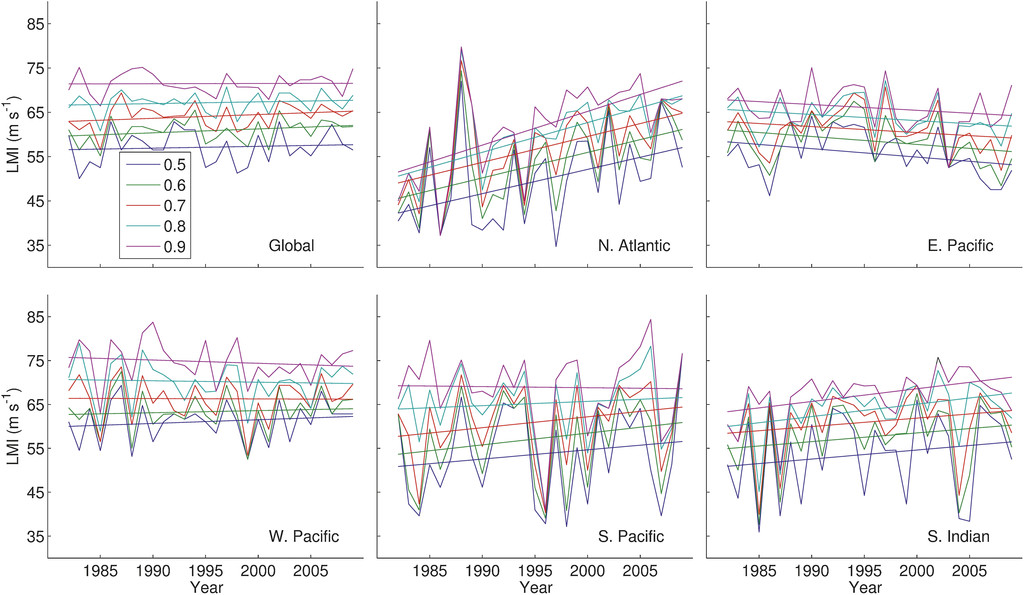
\includegraphics[width=\textwidth]{trends_lmi_kossin_2013.jpg}
    \caption{Évolution temporelle de l'intensité maximale sur le cycle de vie des TC (\textit{lifecycle maximum intensity}, LMI) entre 1982 et 2009, présentée
        par les quantiles entre \num{0.5} et \num{0.9} de la distribution associée et leur tendances linéaires. Intensités calculées avec une base de données
        homogénéisée de l'intensité construite à partir d'images satellites \hbox{HURSAT} (\textit{Hurricane Satellite}) auxquelles est appliquée la technique
        de Dvorak avancée (\textit{Advanced Dvorak Technique}, ADT, \cite{olander_advanced_2007}). Figure issue de \hbox{\cite{kossin_trend_2013}}}
    \label{fig:observed_trends_lmi}
\end{figure}

En dépit de toutes ces difficultés, la mise en commun des données issues de chaque centre spécialisé en un fichier unique est précisément l'objectif de la base
de données IBTrACS (\textit{International Best Track Archive for Climate Stewardship}, \cite{knapp_international_2010}). Bien qu'IBTrACS puisse être moins
détaillée que certaines bases de données locales, comme par exemple HURDAT2 pour l'océan Atlantique \parencite{landsea_atlantic_2013} qui fournit une information
sur la taille des cyclones à travers l'étendue maximale des vents à \num{34}, \num{50} et \SI{64}{\knot} dans les quatre quadrants autour du centre du système,
elle possède donc néanmoins la qualité de couvrir tous les bassins géographiques et fournit également une grande quantité de méta données permettant de filtrer
au mieux les informations. Pour cette raison, IBTrACS est la base de données observationnelle qui est utilisée à travers tout ce document. Il demeure que toutes
les sources d'hétérogénéité mentionnées, spatiales comme temporelles, y compris la rupture causée par l'avènement de l'ère satellitaire, constituent autant de
limites à l'analyse de tendances historiques de l'activité cyclonique tropicale.

\begin{figure}[tb]
    \centering
    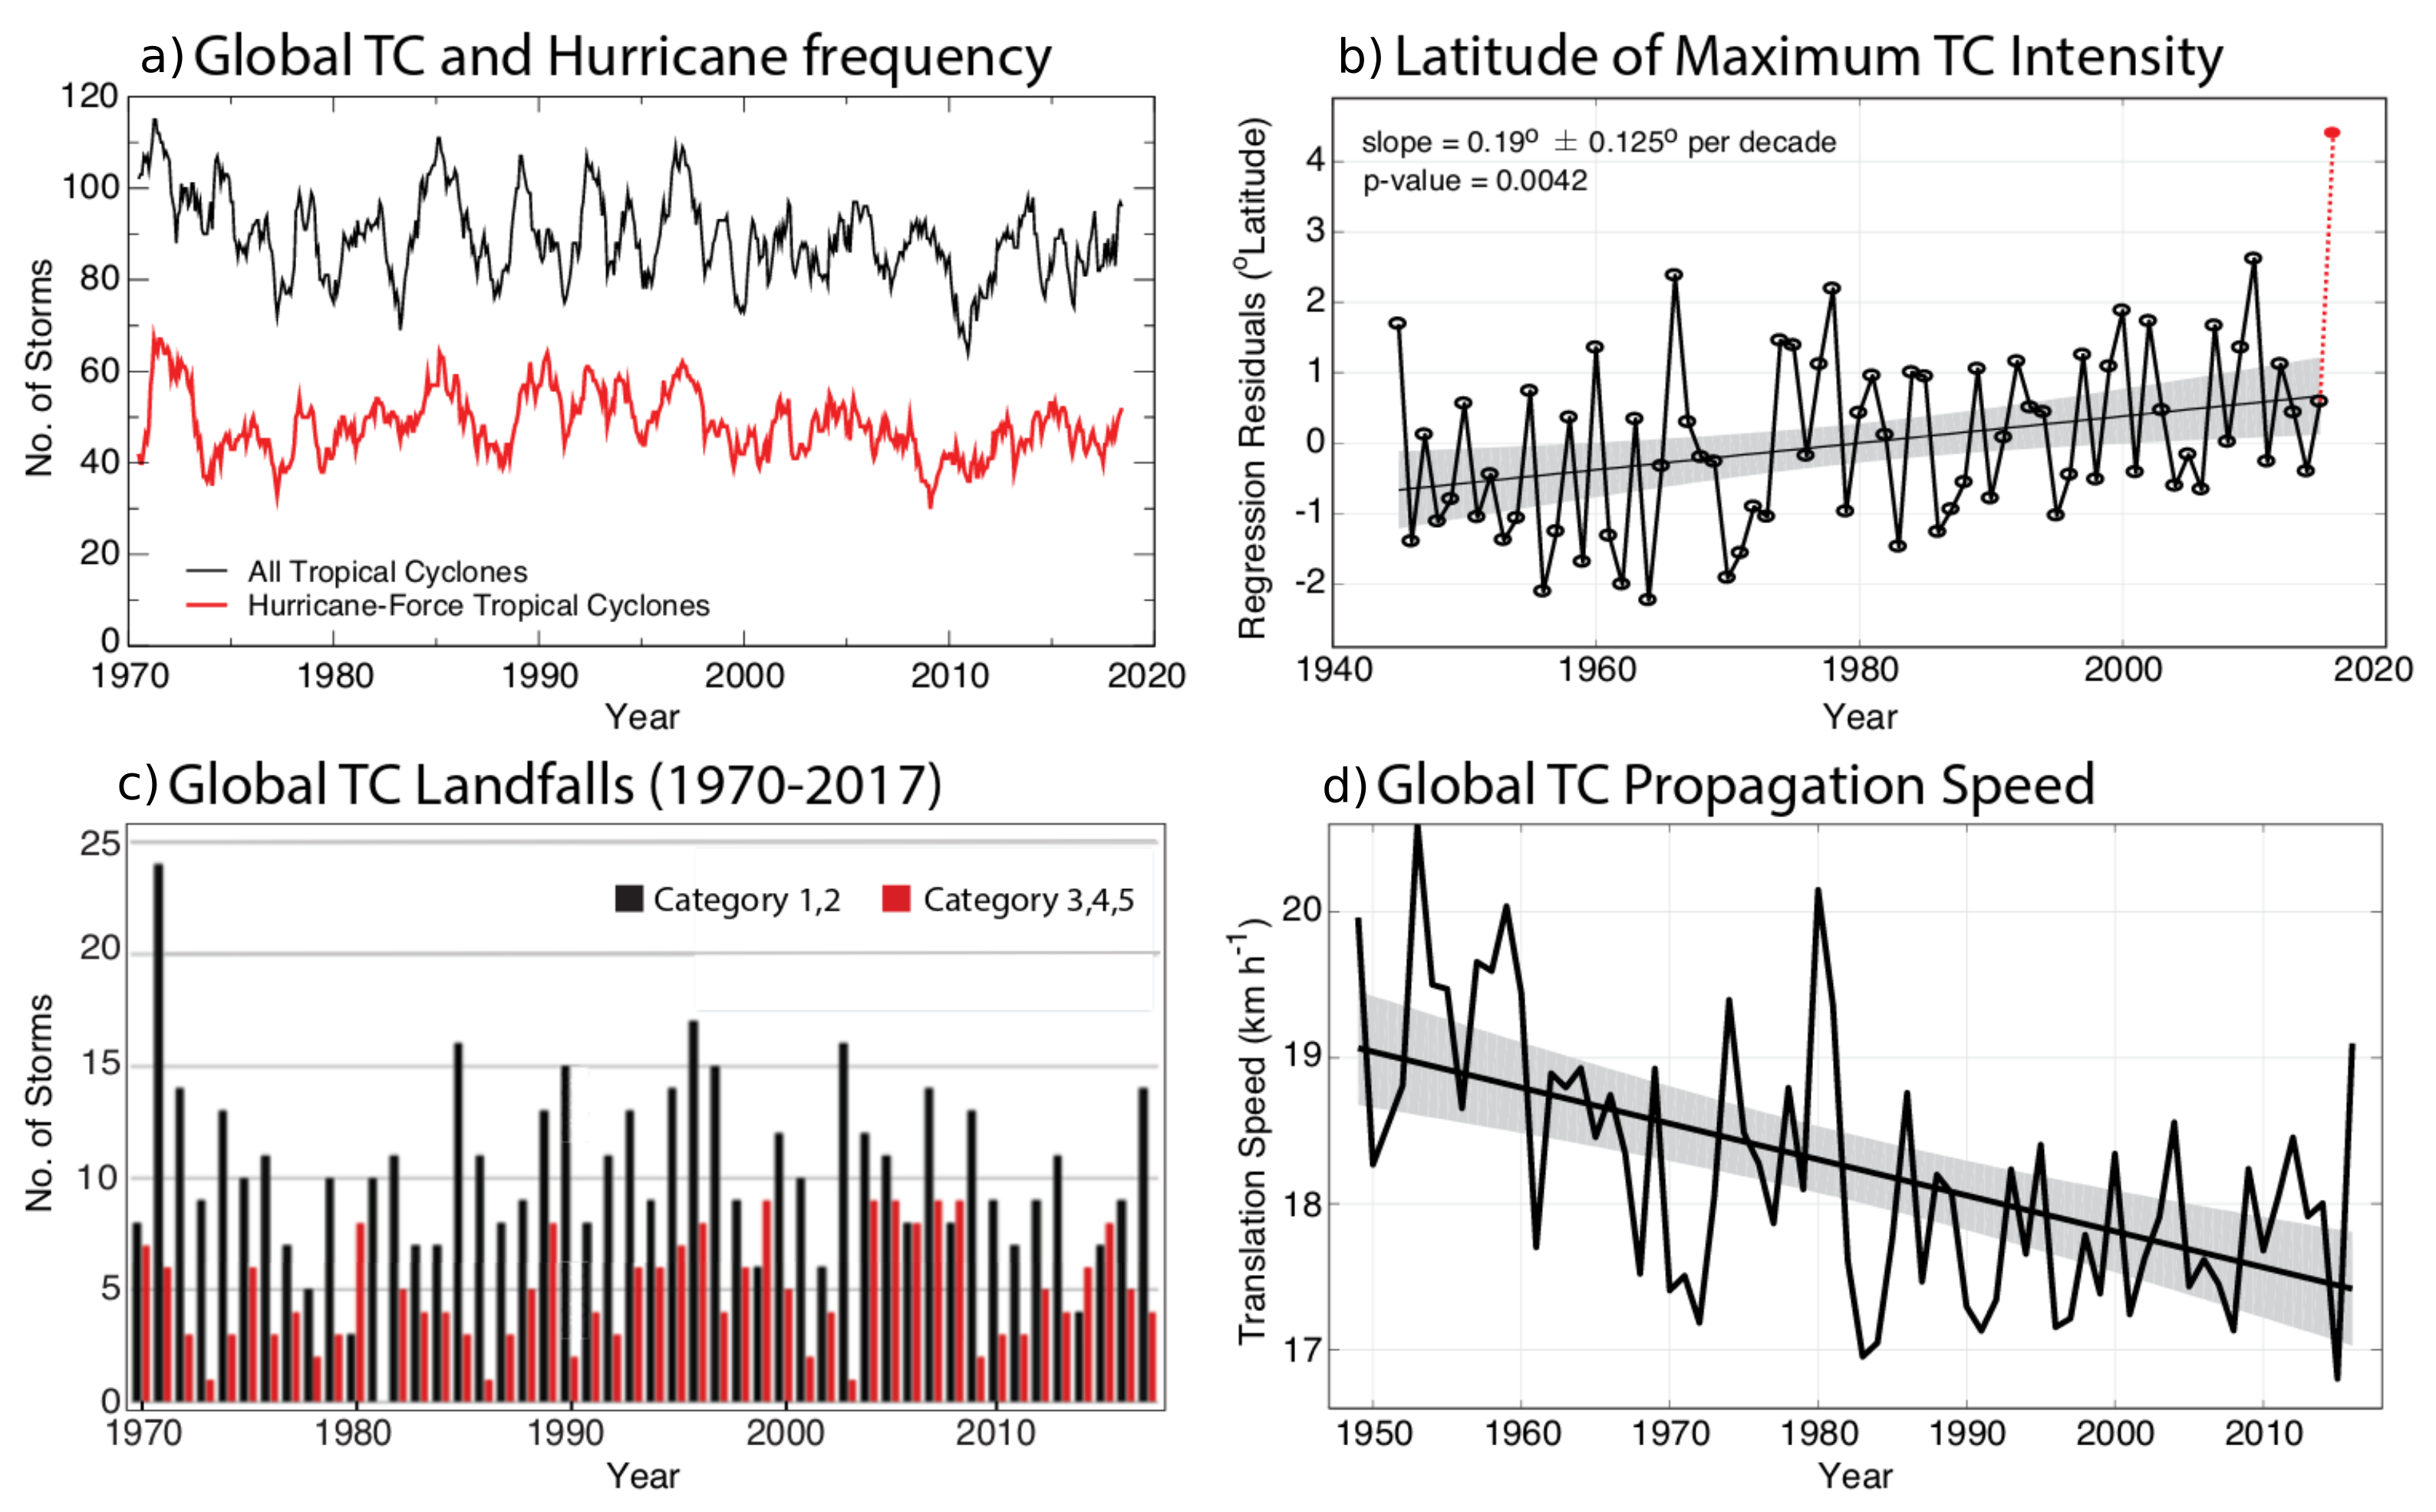
\includegraphics[width=\textwidth]{trends_freq_lat_land_speed_kossin_2019.png}
    \caption{\textbf{(a)} Fréquence globale annuelle des tempêtes tropicales (\SI{34}{\knot}) en noir et des TC atteignant au moins la catégorie 1 en rouge
        (\SI{64}{\knot}) entre 1970 et Mai 2018 et sous forme de somme glissante sur 12 mois \parencite{maue_recent_2011}. \textbf{(b)} Évolution annuelle de la
        moyenne des latitudes auxquelles l'intensité maximale est atteinte dans le bassin WPac, après retranchement de l'influence des modes de variabilité El Niño et de
        l'oscillation décennale du Pacifique par régression linéaire, et intervalle de confiance à \SI{95}{\percent} \parencite{kossin_comment_2018}. \textbf{(c)}
        Fréquence annuelle des TC touchant terre pour les catégories \num{1} et \num{2} (noir) et de \num{3} à \num{5} (rouge) entre 1970 et 2016
        \parencite{weinkle_historical_2012}. \textbf{(d)} Vitesse moyenne globale de translation des TC entre 1949 et 2016 et son intervalle de confiance à
        \SI{95}{\percent} \hbox{\parencite{kossin_global_2018}}. Les encadrés (a) et (c) ont été mis à jour par leurs auteurs respectifs dans le cadre de
        \cite{knutson_tropical_2019}, étude dont sont issues ces quatre figures.}
    \label{fig:observed_trends_other}
\end{figure}

Une des tendances historiques les plus facilement détectables concerne l'intensité des cyclones tropicaux. À partir d'une base de données construite dans un
soucis d'homogénéisation spatiale et temporelle de l'intensité observée des TC issus des best tracks, la \cref{fig:observed_trends_lmi} présente les tendances
dans les quantiles de la distribution de l'intensité maximale des cyclones sur la période \num{1982}~--~\num{2009} et fait apparaître une tendance positive
faible à l'échelle globale, indiquant donc un changement vers des systèmes plus forts \parencite{kossin_trend_2013}. Cette tendance globale cache toutefois de
fortes disparités régionales, avec notamment une très forte tendance positive dans le NAtl ---~pouvant s'expliquer au moins en partie par l'augmentation
constatée des SST dans la région due à la phase ascendante actuelle de l'oscillation atlantique multidécénnale (OAM, ou AMO en anglais)
\parencite{ting_forced_2009}~--- et au contraire une diminution de l'intensité dans le bassin EPac. En répétant l'exercice avec des données étendues jusqu'en
\num{2017}, \cite{kossin_global_2020} confirment une tendance à la hausse dans la probabilité de dépassement des TC majeurs et établit une significativité
supérieure à \SI{95}{\percent} pour l'échelle globale, et de \SI{99}{\percent} pour le NAtl. Parmi les autres bassins, seul le SInd présente une significativité
d'au moins \SI{90}{\percent}. Cette propension vers des cyclones plus intenses est accompagnée d'une augmentation du taux d'intensification des TC ainsi que de
la fréquence de cas d'intensification rapide \parencite{balaguru_increasing_2018,kishtawal_tropical_2012}. Dans le bassin WPac, si aucune tendance très nette
dans l'évolution annuelle du LMI ne se dégage, il existe néanmoins une tendance positive statistiquement significative dans la latitude moyenne à laquelle les
TC atteignent leur maximum d'intensité (\cref{fig:observed_trends_other}, encadré \textbf{b}, \hbox{\cite{kossin_comment_2018}}), avec un degré de confiance
jugé faible quant au  fait que cette tendance puisse être attribuable à des forçages anthropiques \parencite{knutson_tropical_2019}. Le décalage vers les pôles
de l'intensité maximale des TC est également détectable à l'échelle globale \parencite{kossin_poleward_2014}. Il est considéré que la fréquence d'occurrence
globale des cyclones tropicaux ---~présentée sur la \cref{fig:observed_trends_other}, encadré \textbf{a}~--- ne présente pas de tendance à long terme
détectable, mais qu'il existe cependant une augmentation de l'activité dans le bassin NAtl depuis \num{1995}
\parencite{webster_changes_2005,maue_recent_2011,wang_climate_2010,seneviratne_weather_2021}. Néanmoins l'étude plus récente de \cite{klotzbach_trends_2022}
portant sur la période \num{1990}~--~\num{2021} établit une tendance globale à la baisse, portée par une diminution de l'activité dans le WPac plus importante
que la hausse du NAtl, et qui serait liée à une tendance à un état de base plus proche de La Niña depuis \num{1990}, c'est à dire marquée par une anomalie
froide des SST équatoriales dans le Pacifique central. Par ailleurs, si la quantité de TC touchant terre ne présente pas de tendance globalement, une tendance à
la baisse est reconnue en Australie de l'est depuis la fin du \num{19}\ieme~siècle \parencite{knutson_tropical_2019,callaghan_variability_2011}. Enfin,
\cite{kossin_global_2018,kossin_reply_2019} a établi une tendance significative à une baisse de la vitesse de translation des TC, présentée sur la
\cref{fig:observed_trends_other}, encadré \textbf{d} et évaluée à \SI{10}{\percent} entre \num{1949} et \num{2016}. Un ralentissement des TC pourrait avoir des
conséquences désastreuses dans la mesure où ces derniers auraient alors plus de temps pour causer des dégâts dans les zones habitées. Bien que ce résultat ait
été repris dans des rapports de référence \parencite{knutson_tropical_2019,seneviratne_weather_2021}, il est néanmoins contesté, notamment par
\cite{lanzante_uncertainties_2019,moon_climate_2019} qui estiment d'une part que cette tendance pourrait être causée par l'hétérogénéité des données, et
plus spécifiquement par l'introduction de données satellitaires à partir de \num{1965}, et d'autre part parce que le ralentissement concernerait d'avantage les
systèmes les plus éloignés de l'équateur, c'est à dire ceux qui sont en général les moins forts.

\subsection{Les modèles de climat}\label{sec:modèles}

Le terme \textquote{modèle de climat} est vaste puisqu'il en existe une très large variété, de complexités différentes, selon les besoins et les questions que
l'on souhaite élucider. Dans le cas de l'étude des cyclones tropicaux, il s'agit de modèles de circulation atmosphérique, qui peuvent soit fonctionner de
manière dite forcée, ou bien de manière dite couplée. Dans le premier cas, les conditions aux limites, à la surface (SST, flux d'échange de chaleur et de matière avec
l'océan...), sont prescrites (on parle aussi de couplage \textit{offline}) et l'atmosphère ne peut donc pas influencer l'océan en retour. Dans le second cas
(aussi appelé couplage \textit{online}), le modèle atmosphérique tourne en parallèle d'un modèle océanique de telle façon à pouvoir représenter les diverses
rétroactions. Ces modèles sont des programmes informatiques qui simulent l'évolution de variables atmosphériques (température, pression, humidité...) à un pas
de temps régulier, sur chacune des mailles composant la grille du modèle, et ce en suivant les lois de la dynamique et de la physique atmosphérique. La partie
dynamique du modèle consiste en la résolution à chaque pas de temps des équations de la mécanique des fluides décrivant la circulation atmosphérique, tandis que la
physique et les processus prenant place à une échelle caractéristique plus petite que la taille d'une maille sont paramétrisés. Les modèles de climat peuvent
soit simuler l'atmosphère sur l'entièreté du globe, auquel cas il s'agit de modèles de circulation globaux (\textit{Global Circulation Model}, GCM), ou bien ne
simuler qu'un domaine spécifique~---~il s'agit alors de modèles à aire limitée, ou modèles régionaux (\textit{Regional Circulation Model}, RCM).

\begin{figure}[t]
    \centering
    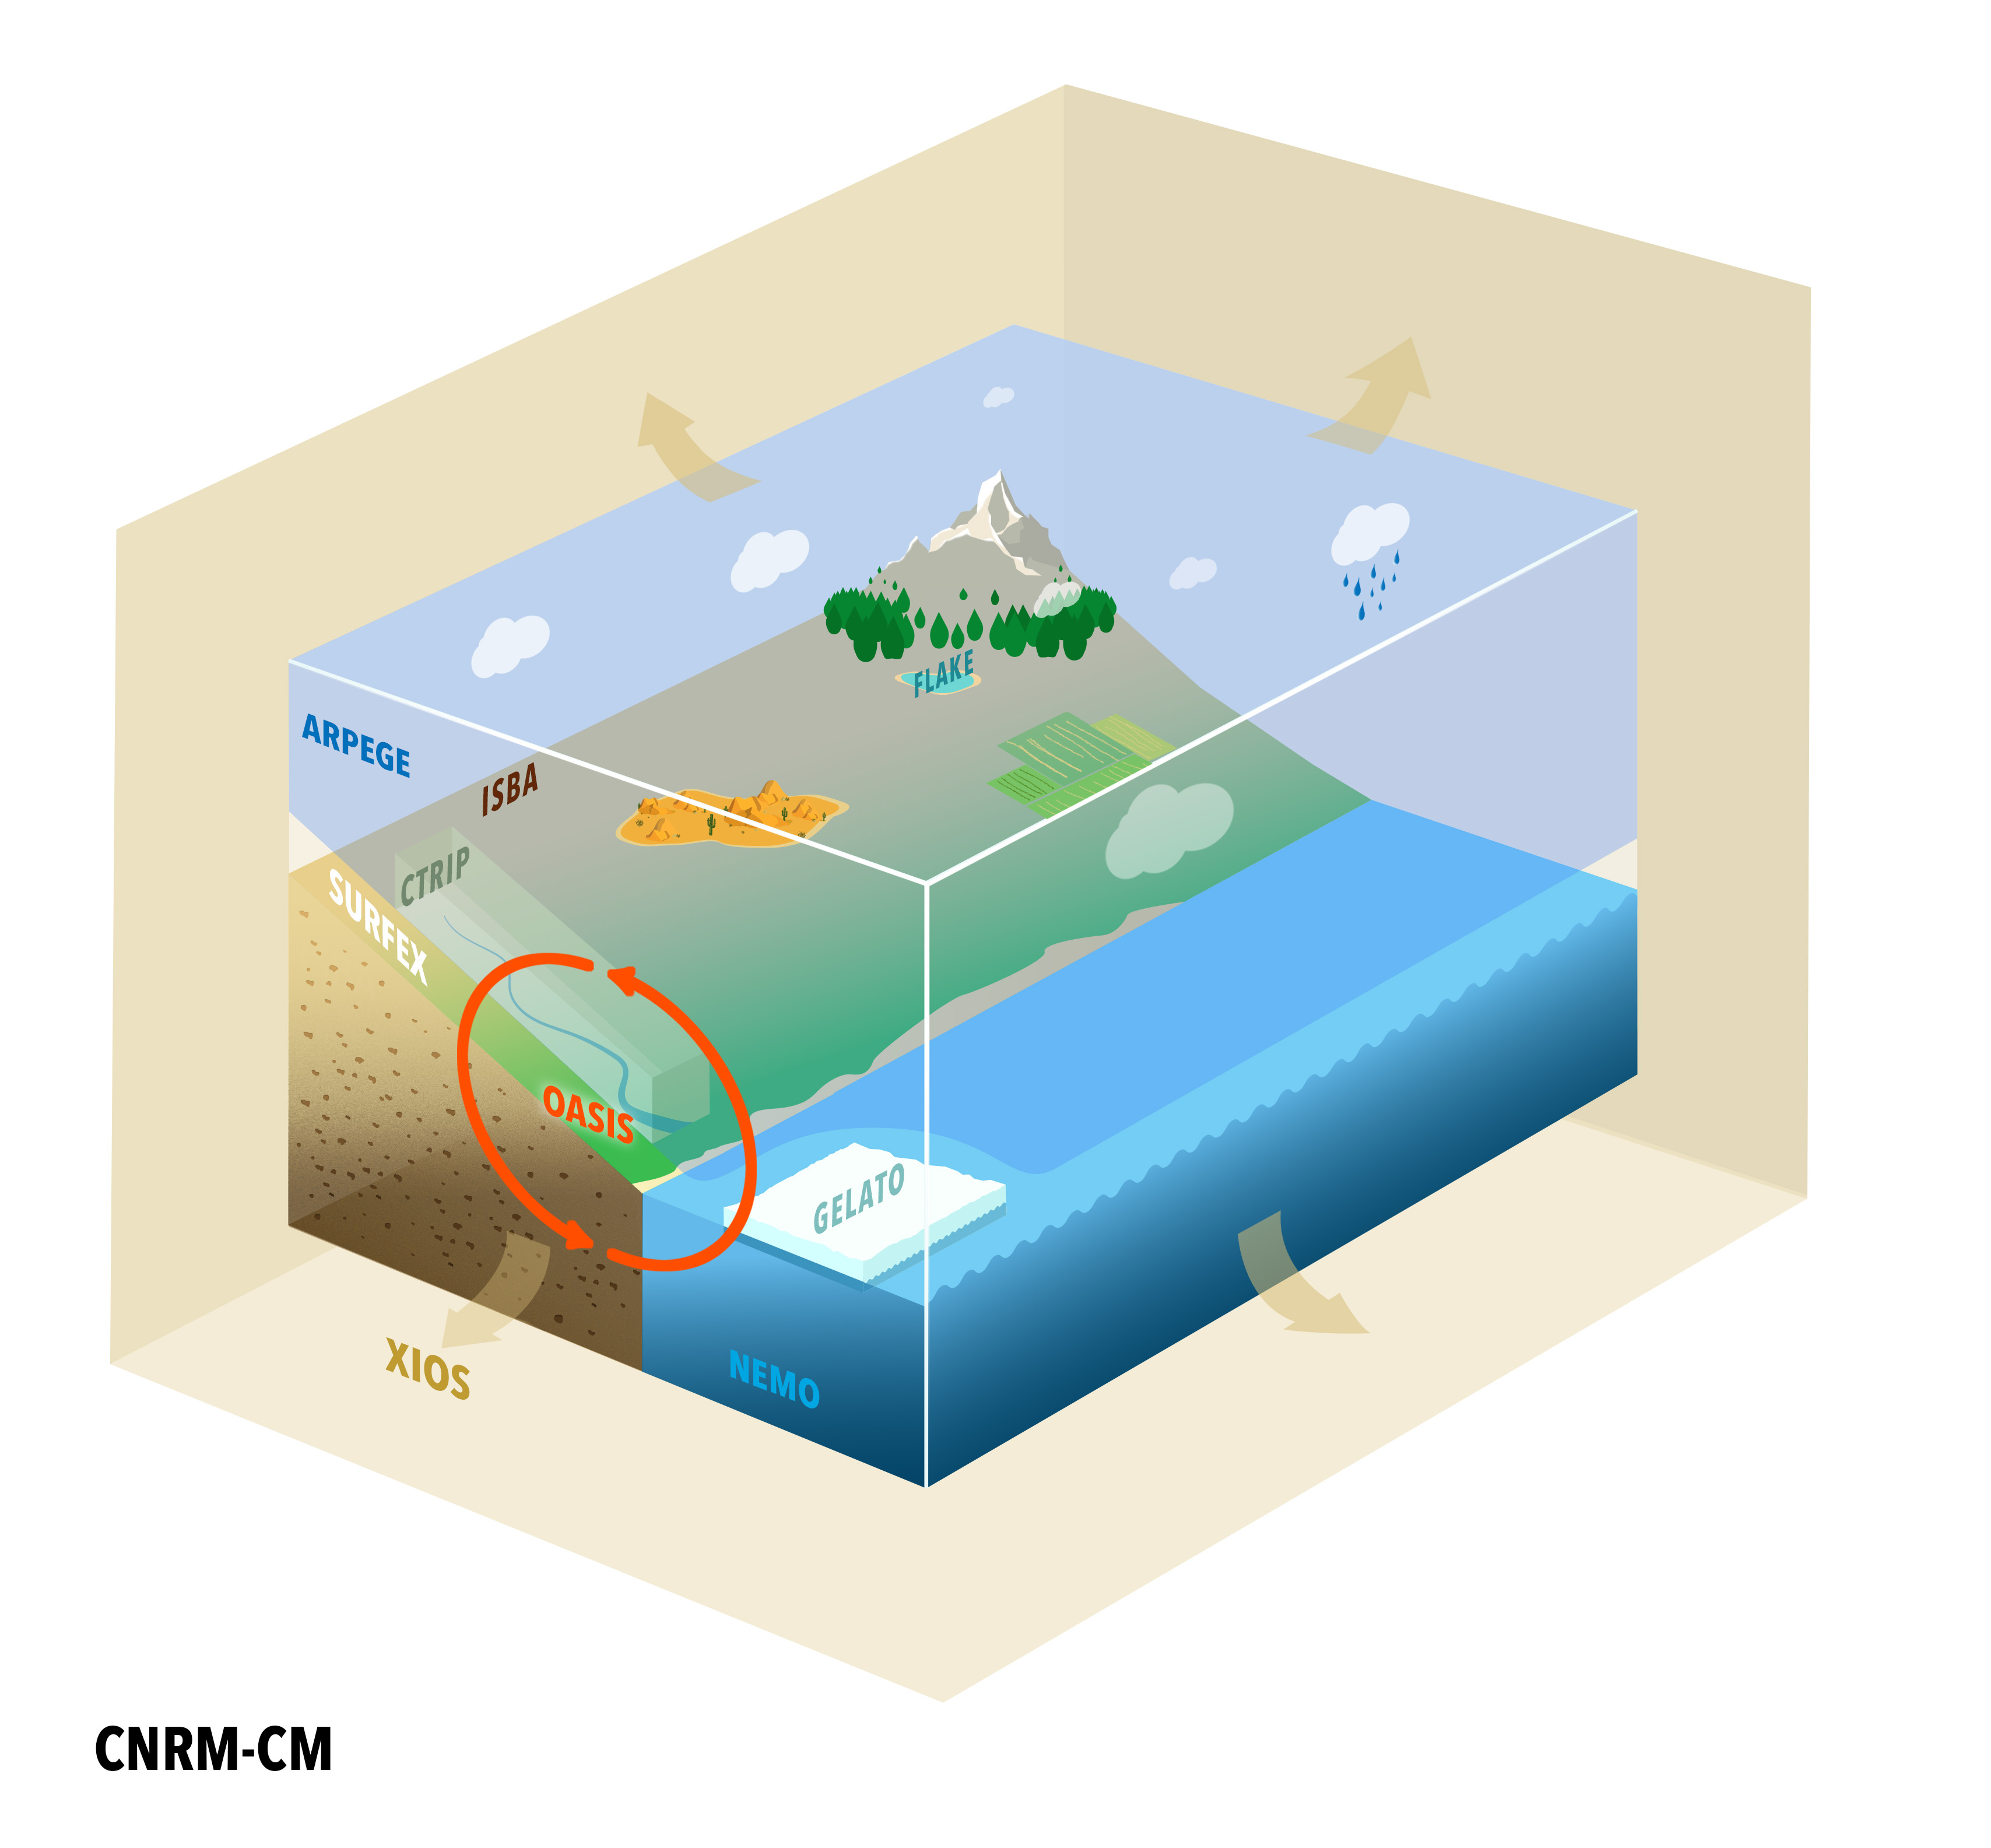
\includegraphics[width=0.9\textwidth]{cnrm-cm6.jpg}
    \caption{Représentation schématique du modèle couplé océan-atmosphère CNRM-CM6-1. \hbox{ARPEGE} constitue la composante atmosphérique de CNRM-CM, ainsi que
    celle du modèle système-terre CNRM-ESM \parencite{seferian_evaluation_2019}. Illustration issue de \cite{voldoire_evaluation_2019}.}
    \label{fig:cnrm-cm6}
\end{figure}

Au CNRM, le modèle atmosphérique global est nommé ARPEGE-Climat \parencite[Action de Recherche Petite Échelle Grande Échelle,][]{deque_arpege_1994} et est
dérivé du modèle de prévision numérique du temps ARPEGE/IFS \parencite[\textit{Integrated Forecast System},][]{courtier_arpege_1991}, développé conjointement
par Météo-France et le CEPMMT. En tant que composante atmosphérique dans le modèle couplé océan-atmosphère \nolinebreak CNRM-CM6-1
\parencite{voldoire_evaluation_2019}, ARPEGE est doté d'une résolution horizontale d'environ \ang{1.4} à l'équateur, ou approximativement \km{140}, et \num{91}
niveaux verticaux. Cela situe donc ARPEGE à peu près dans la moyenne des modèles globaux modernes puisque la résolution des modèles atmosphériques ayant pris
part au sixième et plus récent exercice d'intercomparaison des modèles couplés (\textit{Coupled Model Intercomparison Project}, CMIP, ici CMIP6)
\parencite{eyring_overview_2016} varie entre \km{80} et \km{250} \parencite[][Tableau AII.5]{ipcc_annex_2021}. Une version dite haute-résolution du modèle
ARPEGE existe néanmoins et est utilisée dans le modèle couplé CNRM-CM6-1-HR \parencite{saint-martin_tracking_2021}, participant au projet d'intercomparaison des
modèles haute résolution (\textit{High Resolution Model Intercomparison Project}, HighResMIP) \parencite{haarsma_high_2016} et fonctionnant à une résolution
horizontale de \km{50} ---~les autre modèles participants se situant entre \km{20} et \km{80} \parencite[][Tableau AII.6]{ipcc_annex_2021}. Ainsi, de manière
générale un GCM disposant d'une résolution horizontale plus fine que \km{100} peut être considéré comme un modèle de climat à haute résolution. La finesse de la
résolution des modèles de climat est en pratique limitée par le temps de calcul nécessaire à leur fonctionnement, et la résolution relativement grossière des
modèles de climat modernes témoigne de l'importance de leurs besoins en puissance de calcul, puisqu'il est aujourd'hui difficile de produire des simulations
climatiques de l'ordre d'une centaine d'années avec une résolution en dessous de \km{50} en un temps de calcul raisonnable, malgré la grande capacité des
supercalculateurs\footnote{Le supercalculateur sur lequel ARPEGE-Climat opère actuellement, nommé Belenos, occupait la \num{55}\ieme~place du classement mondial
lors de sa mise en fonctionnement en Juin \num{2021} \parencite{belenos_top500}.}.

La résolution d'un modèle est déterminante dans sa capacité à simuler une activité cyclonique réaliste \parencite{roberts_impact_2020}, aussi bien pour ce qui
est de la fréquence d'occurrence que pour l'intensité des systèmes simulés, puisqu'il est estimé qu'un modèle doté d'une résolution plus large que \km{25} ne
saurait produire une quantité réaliste de cyclones de catégorie 4 sur l'échelle de Saffir-Simpson \parencite{davis_resolving_2018}, ce qui laisse entendre que
la majorité des GCM à haute résolution n'en sont donc pas capables. Il est cependant possible d'accroître la résolution des modèles de circulation
atmosphérique. Une des solutions consiste à utiliser un modèle dit à aire limitée (RCM). En ne simulant l'évolution de l'atmosphère que sur un domaine
restreint, ces derniers sont en mesure d'opérer à des résolutions nettement plus fines avec des temps de calcul raisonnables, typiquement de l'ordre de \km{25}
sur des bassins cycloniques \parencite{redmond_projected_2015,gallo_highresolution_2019,torres-alavez_future_2021}. Toutefois, un RCM ne peut pas fonctionner de
manière purement autonome car il a besoin de connaître l'état de l'atmosphère aux limites de son domaine. Ces informations sont fournies par un autre modèle qui
l'englobe, souvent un GCM, ou parfois même un autre RCM si le saut de résolution est trop important (constituant donc une chaîne à trois modèles). La
cohabitation nécessaire entre le RCM et son GCM forceur n'est pas sans inconvénients, car le RCM est alors très sensible à ces conditions aux limites
\parencite{wu_estimating_2005} et donc au choix du GCM. De plus, les différences dans la dynamique et la physique entre le GCM et le RCM font que la cohérence
entre la grande et la fine échelle n'est pas forcément assurée entre les deux composants, incohérence illustrée par exemple avec la sous-estimation dans les RCM
de la réponse au forçage anthropique suggérée par les GCM sur l'Europe continentale \parencite{boe_large_2020,taranu_mechanisms_2023}. Le gain de résolution
apporté par l'utilisation de modèles à aire limitée est donc contrebalancé par l'introduction de nouvelles incertitudes et difficultés associées.

\begin{figure}[tb]
    \centering
    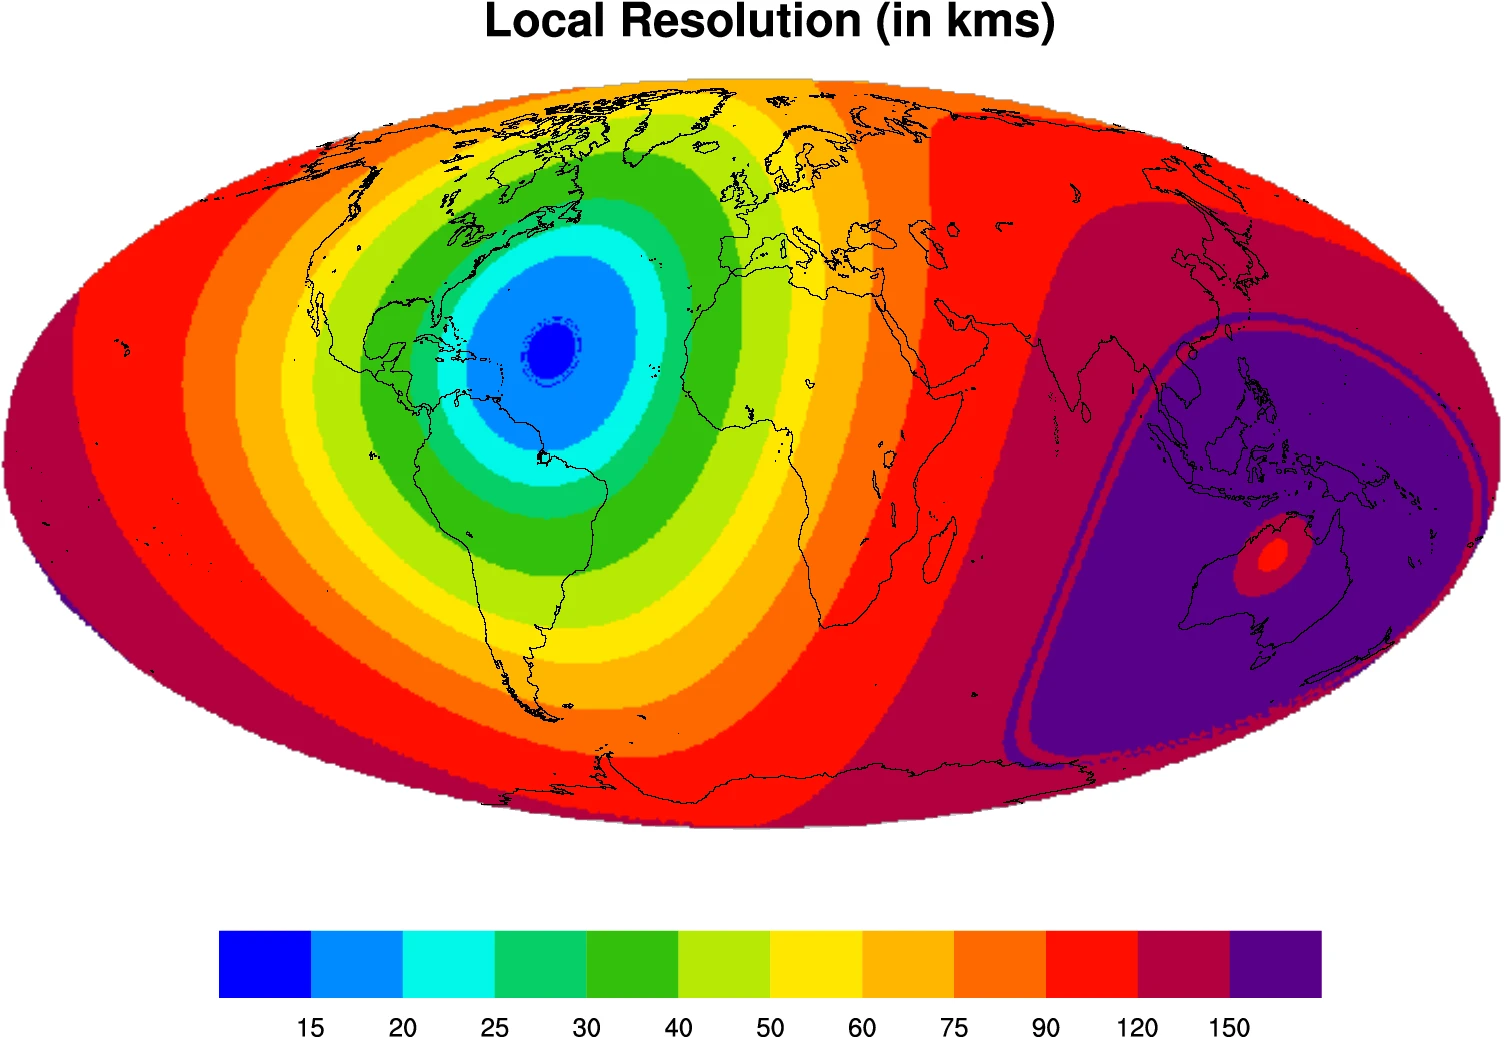
\includegraphics[width=0.8\textwidth]{grille_arpege_stretchee_C3AF.png}
    \caption{Exemple d'utilisation de la grille ARPEGE dans sa configuration basculée-étirée, où le pôle est positionné sur une région d'intérêt et un facteur
    d'étirement est appliqué pour y augmenter localement la résolution (ici égal à \num{3.5}) au détriment de l'antipode. Figure issue de
    \cite{chauvin_future_2020}.}
    \label{fig:rotated_streched}
\end{figure}

Comme alternative aux modèles à aire limitée pour bénéficier d'une résolution accrue, le modèle ARPEGE dispose de la capacité de déformer sa grille horizontale
afin d'augmenter significativement sa résolution sur une région d'intérêt \parencite{courtier_global_1988}. Pour ce faire, le pôle de la grille est
placé sur la région désirée avant d'appliquer la transformation de \cite{schmidt_variable_1977} avec un facteur d'étirement $c$. Si \cite{caian_limits_1997}
ont montré que la précision du modèle demeurait bonne jusqu'à un facteur $c=7$ ---~au delà de quoi l'usage d'un RCM peut être préférable~--- l'étirement est en
pratique souvent limité à \num{3.5}, valeur pour laquelle le modèle a initialement été validé pour la prévision opérationnelle du temps à court terme
\parencite{benichou_validation_1992}. Cette capacité permet à ARPEGE d'atteindre localement jusqu'à \km{14} de résolution à l'emplacement du pôle, avec un
minimum de \km{35} sur un bassin comme le NAtl \parencite[][c.f \cref{fig:rotated_streched}]{chauvin_future_2020} et de \km{50} sur un bassin plus large comme
le SInd \parencite{cattiaux_projected_2020}\footnote{Dans \cite{cattiaux_projected_2020}, le pôle est placé de façon à maximiser la résolution autour de l'île
de La Réunion, au détriment des côtes Ouest de l'Australie. Il serait sinon possible de garantir une résolution inférieure à \km{40} sur l'ensemble du bassin.}.
La spécificité de sa grille place ARPEGE dans le cercle très restreint des GCM à résolution variable, puisqu'ils sont au nombre de cinq
\parencite{mcgregor_recent_2013}, et ARPEGE est le premier d'entre eux à avoir été utilisé pour réaliser des simulations climatiques
\parencite{deque_high_1995}. Cette technique a été maintes fois employée pour l'étude des cyclones tropicaux
\parencite{chauvin_response_2006,chauvin_atlantic_2017,chauvin_future_2020,daloz_impact_2012,cattiaux_projected_2020}, y compris en changement climatique, et
permet donc de profiter des bénéfices de la haute résolution sur un domaine cible donné sans les inconvénients des modèles à aire limitée.

\subsection{Les cyclones dans les modèles de climat}\label{sec:cyclones_dans_modèles}

\cite{manabe_tropical_1970} ont pour la première fois observé, dans une simulation produite par un GCM doté d'une résolution horizontale de \km{417} à
l'équateur, des vortex pouvant s'apparenter à des cyclones tropicaux sous la forme de très larges dépressions atmosphériques de l'ordre de \km{2000} à \km{3000}
de diamètre dans le Sud-ouest de l'océan indien et dans le Pacifique Sud, à des emplacements correspondant aux zones de formation des TC de l'hémisphère sud
identifiées par \cite{gray_global_1968} (voir aussi \cref{fig:produit_ingredients}). Limitées par la résolution du modèle, les dépressions tropicales de
\cite{manabe_tropical_1970} atteignent une vitesse de vent maximale de \ms{20}, soit un stade de tempête tropicale, et ne peuvent pas s'intensifier au delà.
\cite{bengtsson_simulation_1982} ont ensuite proposé une étude plus approfondie des divers stades de développement des TC simulés dans le modèle opérationnel du
CEP, à environ \km{200} de résolution, dans lequel ces objets atteignent un vent tangentiel maximum de \ms{25}. Outre la taille et l'intensité des systèmes
simulés, et malgré une structure interne réaliste lorsque les systèmes sont pleinement développés, \cite{mcbride_comments_1984} souligne plusieurs autres
différences clefs entre les simulations et les TC observés, notamment pendant les étapes de formation et d'intensification, marquées par une très forte activité
convective néanmoins accompagnée d'une absence de cœur chaud et d'une faible vorticité. L'auteur souligne également le lien exacerbé entre la SST et l'activité
simulée, en dépit des autres facteurs favorables à la cyclogénèse identifiés par \cite{gray_tropical_1975} (voir \cref{sec:conditions_cyclogenese}), et
qui explique la répartition spatiale et temporelle imparfaite de l'activité simulée. La faible résolution des GCM et la paramétrisation nécessaire de la
physique sous-maille rendent les TC très difficile à simuler correctement, si bien que la dénomination de HTV
(\textit{Hurricane-Type Vortices}) est parfois préférée pour les désigner
\parencite{bengtsson_simulation_1982,bengtsson_hurricanetype_1995,chauvin_response_2006}.

\begin{figure}[htbp]
    \centering
    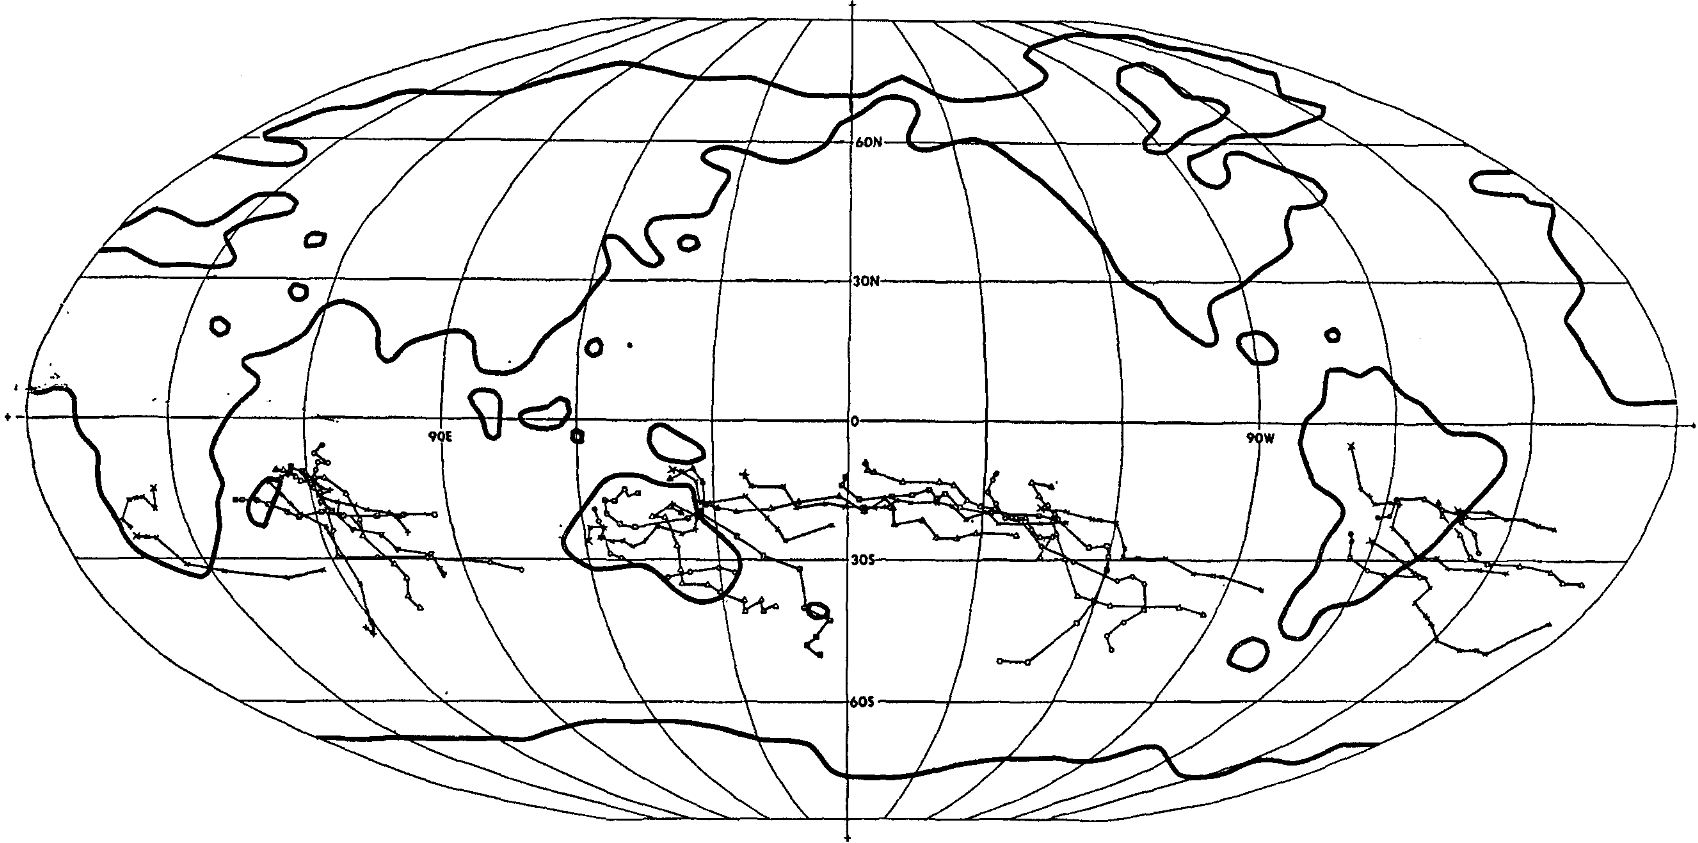
\includegraphics[width=0.9\textwidth]{manabe_1970_tracks_screenshot.png}
    \caption{Trajectoires des HTV détectés par \cite{manabe_tropical_1970}, caractérisés par une dépression centrale d'au moins \hPa{2}. Les croix désignent les
        premières positions des HTV, tandis que les symboles représentent leurs positions respectives avec un intervalle de \SI{24}{\hour}.}
    \label{fig:tracks_manabe}
\end{figure}

\cite{broccoli_can_1990} ont ensuite pour la première fois essayé d'utiliser un modèle de climat pour étudier l'influence du changement climatique sur
l'activité cyclonique, en analysant les HTV dans le modèle du GFDL (\textit{Geophysical Fluid Dynamics Laboratory}) via des expériences à deux résolutions
différentes (\ang{4.5}\times\ang{7.5} et \ang{2.25}\times\ang{3.75}, en latitude et longitude, respectivement), \num{9} niveaux verticaux, avec et sans
rétroactions nuageuses et dans lesquelles la concentration en \ce{CO2} est doublée. Ils notèrent ainsi un changement à la baisse en
\ensuremath{2\times\ce{CO2}} dans la simulation avec rétro-action nuageuse, et au contraire une augmentation lorsque la nébulosité est prescrite, indépendamment
de la résolution utilisée. Ces expériences, bien que peu concluantes, validèrent le principe de l'utilisation de GCM pour l'étude des TC en changement
climatique. \cite{haarsma_tropical_1993,bengtsson_will_1996} procédèrent à de nouvelles expériences en \ensuremath{2\times\ce{CO2}} et notèrent tous deux une augmentation
relative de la fréquence des cyclones les plus forts tandis que \cite{bengtsson_will_1996} observa également une réduction de l'activité dans la
simulation \ensuremath{2\times\ce{CO2}}. Une réduction de l'activité cyclonique accompagnée d'une augmentation relative de la fréquence d'occurrence des TC les
plus forts constitue un signal robuste de réponse au changement climatique encore aujourd'hui \parencite[][voir
\cref{sec:projections_futures}]{walsh_tropical_2016,camargo_tropical_2016,knutson_tropical_2010,knutson_tropical_2010,seneviratne_weather_2021}. À la même
époque, \cite{bengtsson_hurricanetype_1995} notèrent une forte variabilité inter-annuelle de l'activité cyclonique dans leurs simulations, en dépit du fait que
des SST climatologiques ---~donc dénuées de cette variabilité~--- furent prescrites, et établirent un lien entre l'activité simulée et des modes de circulation
de grande échelle, s'affranchissant ainsi du trop fort lien entre SST et cyclogénèse des HTV dans les premières expériences. Leurs travaux montrèrent également
un lien clair entre la résolution du modèle d'une part, et l'intensité ainsi que le réalisme de la structure interne des HTV d'autre part.

\begin{figure}[tb]
    \centering
    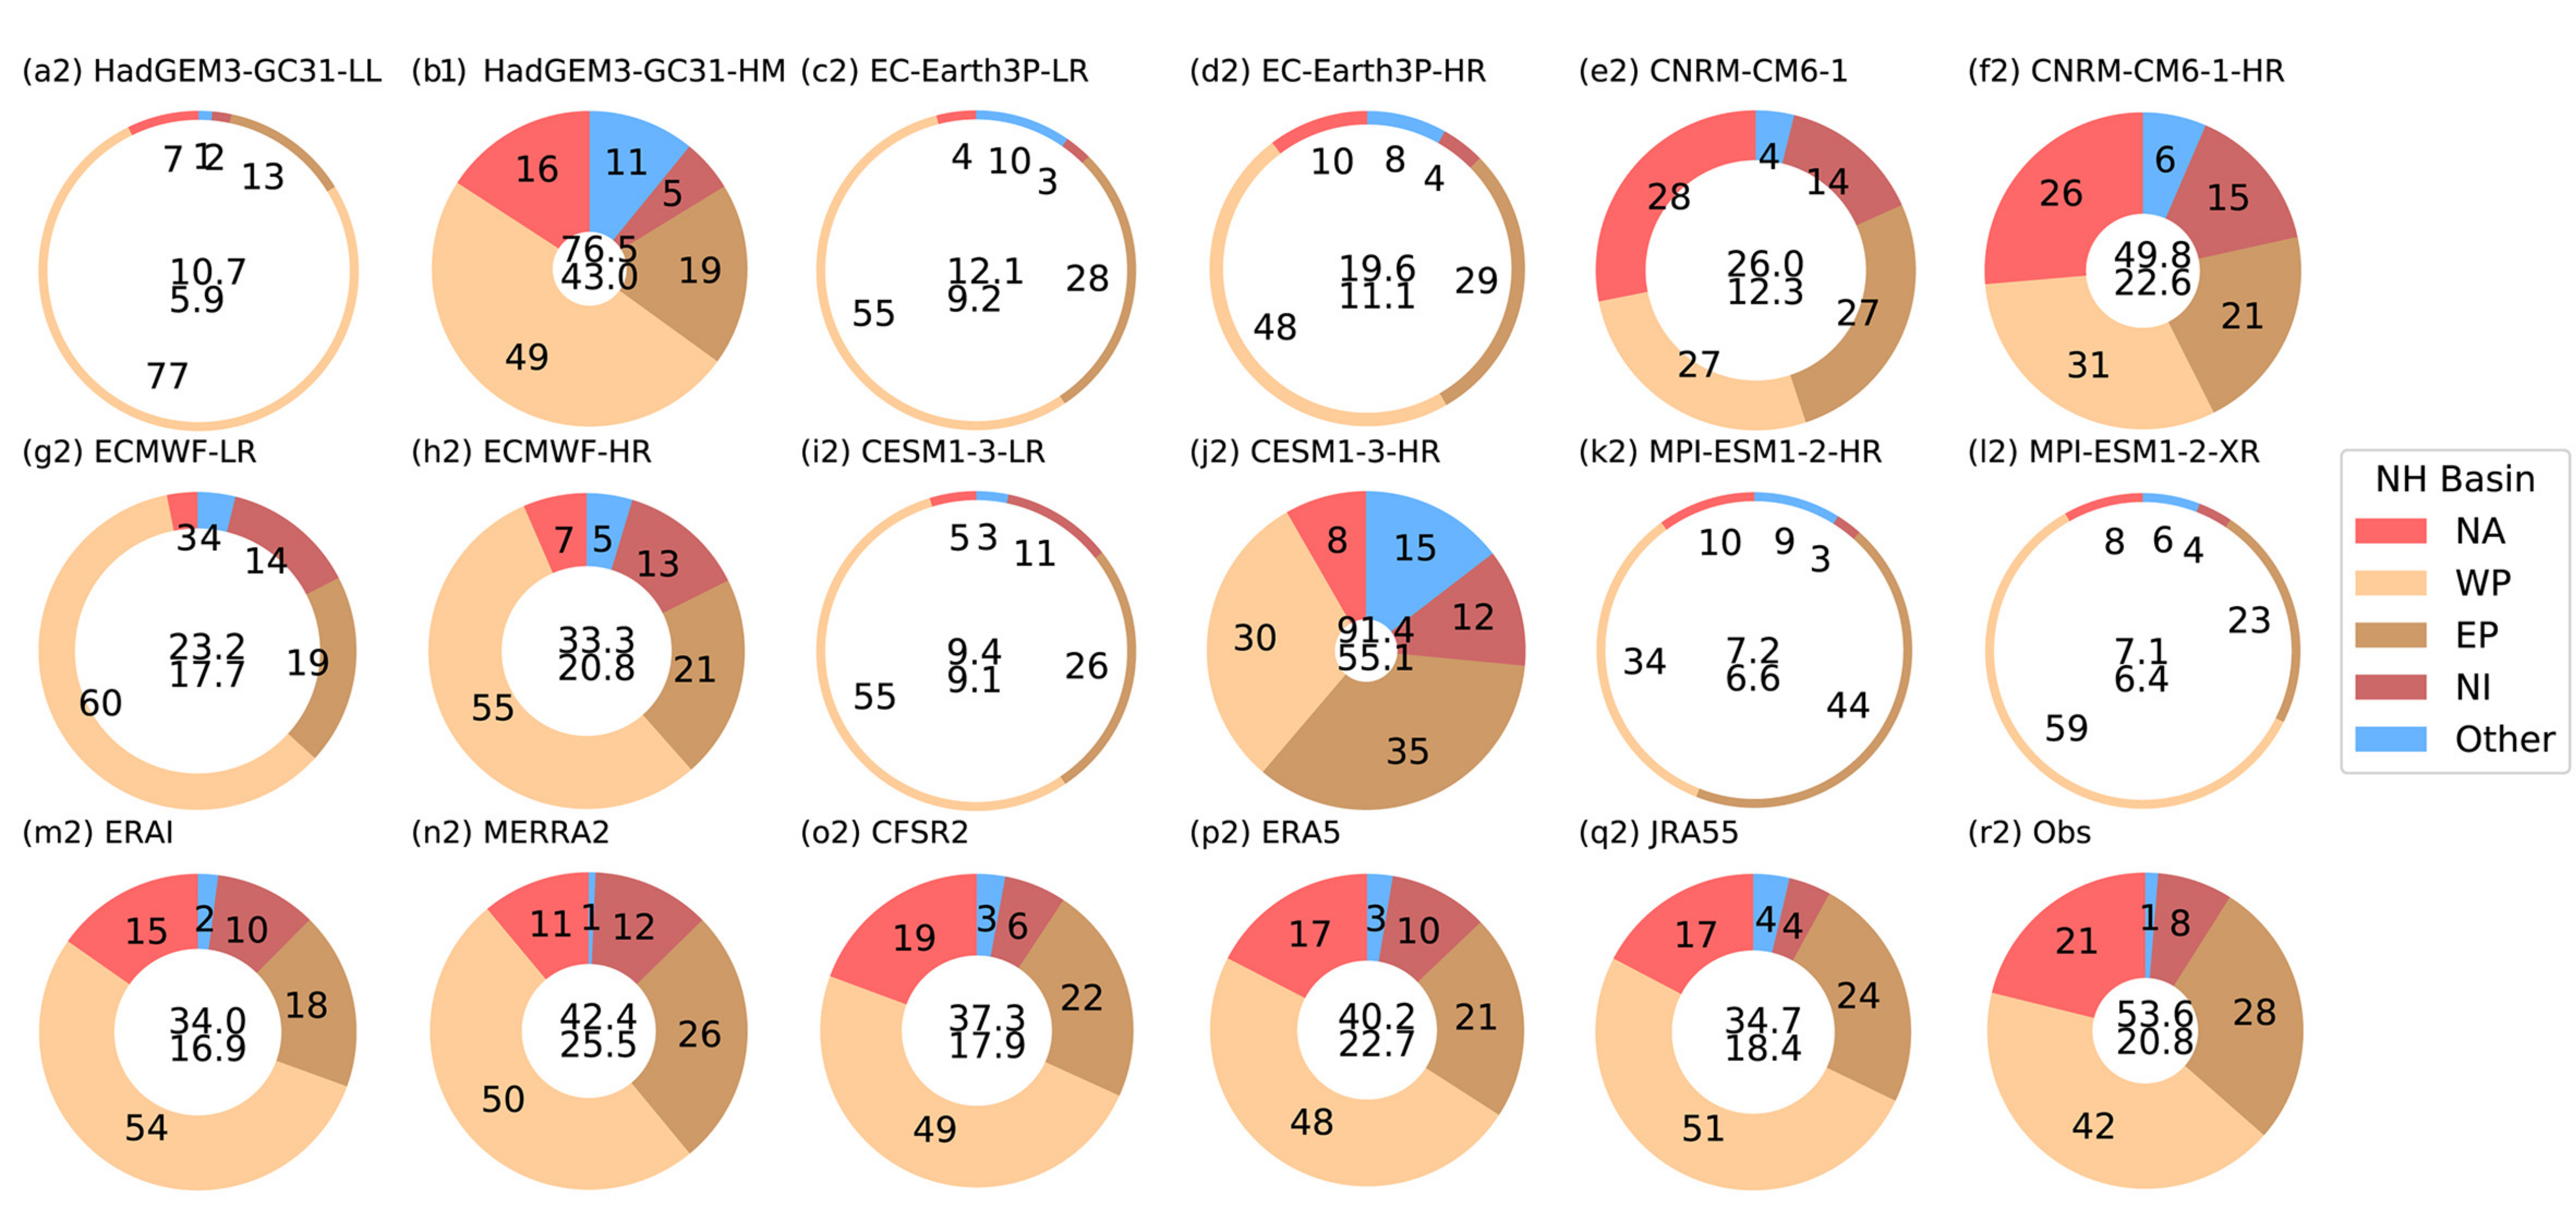
\includegraphics[width=\textwidth]{roberts_projected_2020_TE_coupled.png}
    \caption{Fréquence annuelle moyenne du nombre de TC dans des simulations historiques couplées océan-atmosphère HighResMIP (tiers 2) sur la période
        \num{1974}~--~\num{2014} (deux premières lignes) ainsi que pour cinq réanalyses et dans les observations (dernière ligne). Moyenne annuelle entre Mai et
        Novembre dans l'hémisphère nord et Octobre~--~Mai dans l'hémisphère sud. Les modèles couplés sont par paire basse / haute résolution. Les deux valeurs
        centrales de chaque disque présentent la moyenne dans les deux hémisphères et les tranches de couleur précisent le pourcentage de HTV de l'hémisphère
        nord pour chaque bassin d'activité. L'épaisseur des disques est calibrée sur le nombre annuel de TC observés dans l'hémisphère nord. Figure issue de
        \hbox{\cite{roberts_projected_2020}}.}
        \label{fig:NTC_HighResMIP}
\end{figure}
\begin{figure}[tb]
    \centering
    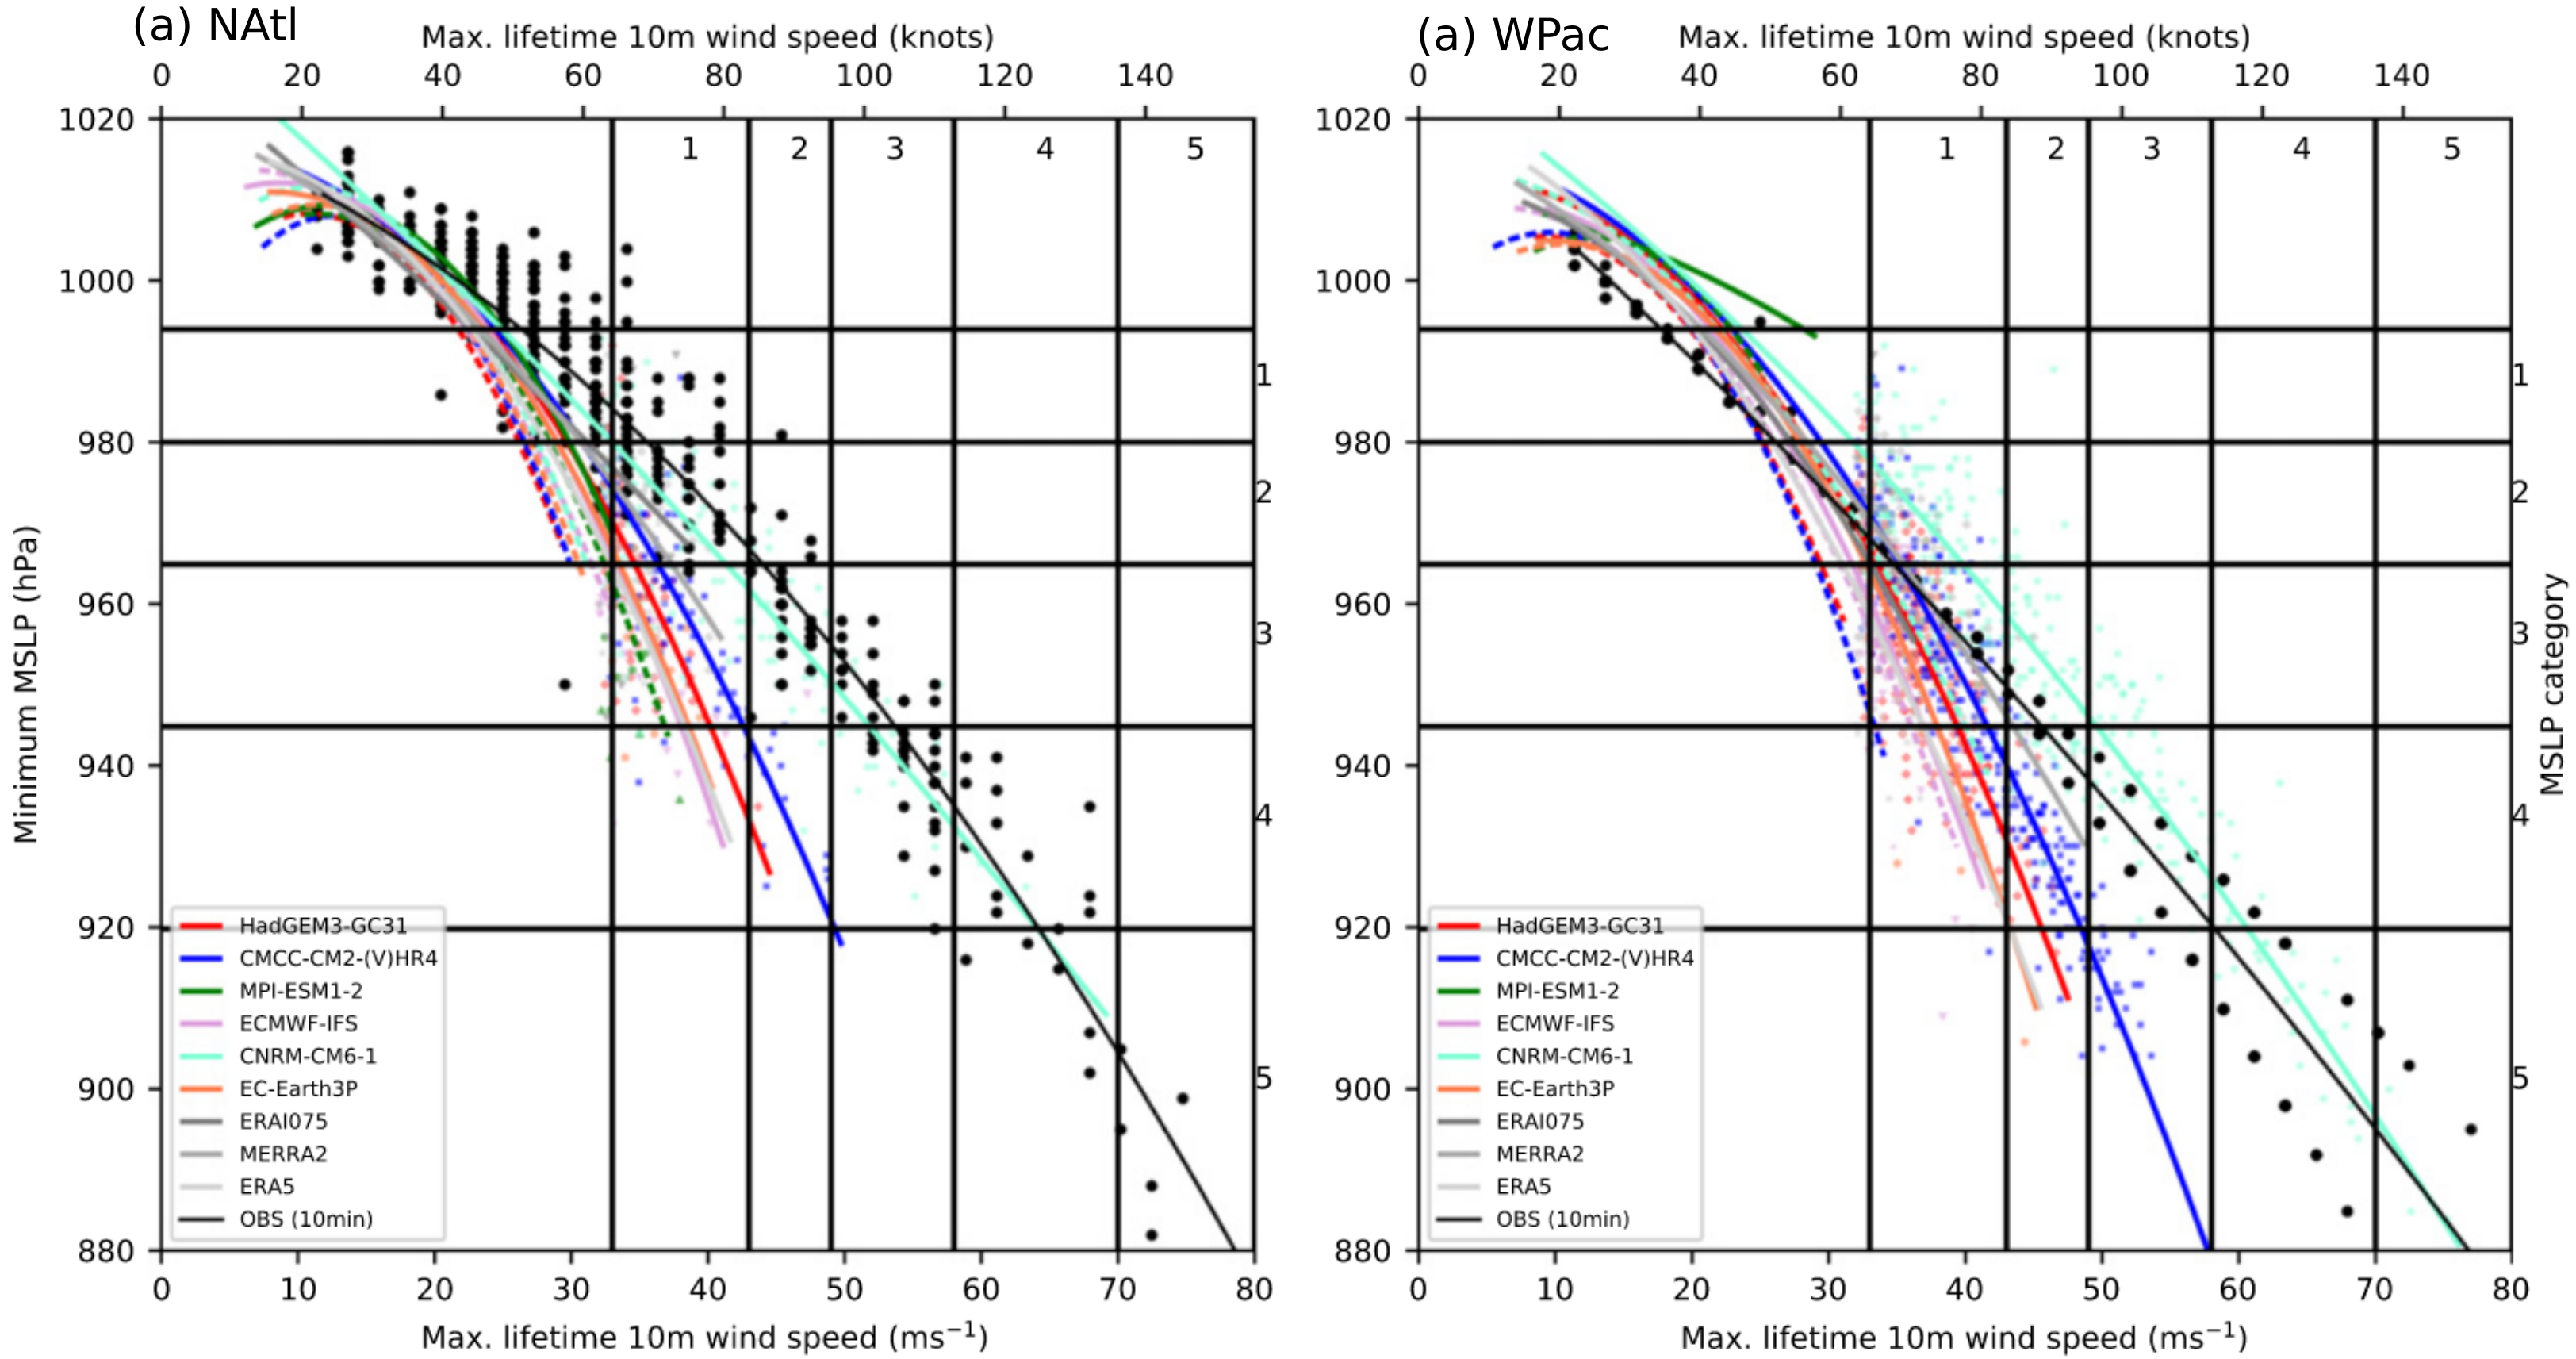
\includegraphics[width=\textwidth]{roberts_impact_2020_PV_NA_WP.png}
    \caption{Diagramme de relations vent~--~pression entre le vent maximum à \m{10} et le minimum de pression moyenne au niveau de la mer (\textit{Mean
        Sea-Level Pressure}, MSLP) dans les bassins Nord Atlantique (a) et Ouest Pacfique (b), pour \num{6} paires de modèles basse / haute résolution dans des
        simulations HighResMIP du tiers \num{1} (Runs atmosphériques forcées), ainsi que pour \num{3} réanalyses (en teintes de gris) et dans les observations
        (en noir). Les lignes pointillées indiquent les régressions pour les modèles basses résolution, et les lignes pleines pour les modèles haute résolution.
        Figure issue de \hbox{\cite{roberts_impact_2020}}.}
    \label{fig:roberts_PV_resolution}
\end{figure}

Les modèles ont depuis continué à s'améliorer, et s'ils souffrent toujours de la sous-estimation de l'intensité maximale, ils sont désormais capables de simuler
l'évolution du cycle de vie des TC, la répartition géographique, la saisonnalité des bassins d'activité ---~avec plus ou moins de succès selon les bassins, et
selon les modèles~---
\parencite{bengtsson_tropical_2007,zhao_simulations_2009,shaevitz_characteristics_2014}, ainsi que l'influence de l'Oscillation australe El Niño sur l'activité cyclonique
\parencite{vitart_simulation_1997,gualdi_changes_2008,camargo_experimental_2009}. La fréquence annuelle globale de HTV dans les GCM est toutefois très variable
selon les modèles, comme en atteste la \cref{fig:NTC_HighResMIP}. La résolution des modèles joue un rôle crucial dans la représentation des TC, y compris dans
la fréquence. La \cref{fig:NTC_HighResMIP} montre en effet que les modèles à plus haute résolution simulent généralement plus de HTV que ceux de résolution
inférieure \parencite{camargo_global_2013,roberts_impact_2020}. Cependant, elle montre aussi que la résolution ne peut expliquer à elle seule la sous-estimation
de la fréquence, puisque deux des paires de modèles sur la \cref{fig:NTC_HighResMIP} ne présentent qu'une amélioration marginale, voire pas d'amélioration dans
leur version haute résolution (EC-Earth3P, \cite{haarsma_highresmip_2020} et MPI-ESM1-2, \cite{gutjahr_max_2019}). La figure met aussi en évidence de fortes
différences de fréquence relatives à l'échelle des bassins géographiques. Le modèle CNRM-CM6-1 est par exemple le seul à surestimer l'activité dans le bassin
NAtl, aussi bien dans sa version basse que haute résolution\footnote{Dans CNRM-CM6-1, la surestimation de la fréquence relative dans le NAtl pour la version basse
résolution semble due au couplage océan-atmosphère, car \cite{roberts_impact_2020,roberts_projected_2020} montrent en effet que l'expérience réalisée avec des
SST prescrites produit une activité relative de \SI{11}{\percent}. En revanche pour les autres modèles, le couplage tend à réduire l'activité dans cette
région.} avec respectivement \SI{28}{\percent} et \SI{26}{\percent}, contre \SI{21}{\percent} dans les observations. La \cref{fig:roberts_PV_resolution}
présente les relations vent~--~pression (\textit{Wind-Pressure Relationship}, WPR) pour les modèles présentés dans la \cref{fig:NTC_HighResMIP}. Les diagrammes
vent~--~pression sont couramment utilisés comme diagnostique pour comparer la relation entre ces deux variables ---~reliées entre elles par l'équilibre du vent
cyclostrophique~--- avec celle issue des observations et mesurée pour la première fois par \cite{atkinson_tropical_1977}. Avec la \cref{fig:roberts_PV_resolution},
\cite{roberts_impact_2020} montre une intensification des HTV lors du passage à des résolutions supérieures, comprises entre \km{25} et \km{50}, sans pour
autant parvenir à reproduire la plage de valeurs observée puisque la plupart des modèles peinent à dépasser la catégorie \num{2}~--~\num{3}. Ici encore, le
modèle CNRM-CM-6-1-HR constitue l'exception en simulant des TC particulièrement intenses, dépassant même les observations dans le bassin WPac. Dans le NAtl,
\cite{chauvin_future_2020} montre que l'intensité des HTV est encore accrue lorsque le modèle est utilisé dans sa configuration basculée-étirée pour atteindre
\km{15} de résolution (voir \cref{fig:rotated_streched}). Ce cas constitue une anomalie, d'autant plus que la version précédente du modèle utilisée dans les
simulations de \cite{daloz_impact_2012} ---~également en configuration basculée-étirée, avec une résolution au pôle de \km{50}~--- ne produit pas de HTV aussi intenses. Cette particularité
serait probablement liée aux différences de paramétrisations physiques entre les deux versions \parencite{chauvin_future_2020}, auquel cas il est possible que la
capacité du modèle ARPEGE à simuler des TC de catégorie \num{4} et \num{5} soit due à de mauvaises raisons. Il est néanmoins à noter que, bien qu'ils soient peu
nombreux, d'autres modèles à très haute résolution sont en mesure d'atteindre de tels niveaux d'intensité. C'est notamment le cas du modèle MRI-AGCM~3.2 avec
sa grille à \km{20} \parencite{murakami_future_2012}, le modèle HiFLOR du GFDL à \km{25} \parencite{murakami_simulation_2015} ainsi que CAM~5.1 dans sa
configuration à \km{25} \parencite{wehner_effect_2014}.

Depuis les premiers HTV simulés de \cite{manabe_tropical_1970}, les modèles se sont très nettement améliorés, autant par l'intermédiaire de l'augmentation de la
puissance de calcul permettant d'atteindre des résolutions de quelques dizaines de kilomètres à l'échelle globale, que par les paramétrisations physiques qui
les composent et le couplage avec diverses composantes, tous deux permettant de mieux décrire les processus inhérents aux cyclones tropicaux, et donc de mieux
les représenter dans les modèles. Si les modèles ne permettent toujours pas, pour la plupart, de reproduire pleinement l'amplitude de l'intensité observée, et
si les différences dans leur capacité à représenter les TC et leur activité sont encore grandes, ils n'ont néanmoins jamais été aussi aptes à
simuler l'activité cyclonique et sa variabilité de manière réaliste qu'aujourd'hui. Les modèles de climat constituent par conséquent le meilleur outil pour
tenter d'évaluer l'impact du réchauffement climatique sur l'activité cyclonique. L'état de l'art sur les projections climatiques de l'activité cyclonique est présenté 
dans la \cref{sec:projections_futures}.

\subsection{Approche directe et indirecte pour l'étude de l'activité cyclonique}\label{sec:tracking_vs_indices}

\subsubsection{Approche directe : Détection et suivi objectif des cyclones tropicaux}\label{sec:intro_tracking}

Il existe plusieurs façons d'évaluer l'activité cyclonique dans les modèles et qui peuvent être classées comme directes ou indirectes. En particulier,
l'approche utilisée pour la description des HTV présentées dans la \cref{sec:cyclones_dans_modèles}, et qui est également implicitement référée dans la
\cref{sec:modèles} lorsqu'il est fait mention de l'importance de la résolution, peut être vue comme la mesure la plus directe possible, puisqu'il s'agit
d'identifier les HTV dans les simulations et d'analyser directement leurs caractéristiques, tels qu'ils sont représentés dans les modèles. Cette façon
de procéder repose sur la capacité à correctement identifier et suivre l'évolution des HTV dans les simulations à l'aide d'un schéma (ou algorithme) de
détection et de suivi objectif, aussi appelés algorithmes de tracking ou encore traqueurs. Basés sur les méthodologies de
\cite{haarsma_tropical_1993,bengtsson_hurricanetype_1995}, ces algorithmes consistent pour la plupart à identifier les points de grille qui satisfont certaines
conditions, exprimées comme des seuils de détection puis à relier les points entre eux de façon à former des trajectoires (tracks). Ces données permettent
ensuite d'analyser le cycle de vie des systèmes et de calculer des statistiques de l'activité cyclonique. Néanmoins, le choix de l'algorithme de tracking peut
avoir un impact considérable sur les résultats d'un tel travail. La \cref{fig:NTC_HighResMIP_TRACK} reproduit l'analyse présentée sur la
\cref{fig:NTC_HighResMIP} avec un schéma de détection différent, et montre des écarts importants non seulement sur la quantité de HTV détectés, mais également
sur leur répartition spatiale, en termes d'activité relative par bassin mais aussi sur le ratio de la fréquence entre les deux hémisphères. Par exemple, là où
le modèle CNRM-CM6-1-HR présente un rapport légèrement supérieur à \num{2} entre les fréquences annuelles de l'hémisphère nord et sud avec TempestExtreme \parencite{ullrich_tempestextremes_2017,zarzycki_assessing_2017} ---~un
ratio très proche de celui observé~--- la différence s'amoindrit lorsque ce dernier est remplacé par TRACK \parencite{hodges_how_2017}. Dans d'autres cas, comme pour le modèle ECMWF-LR,
l'algorithme TRACK indique même une activité plus forte dans l'hémisphère sud que dans le nord.

\begin{figure}[htbp]
    \centering
    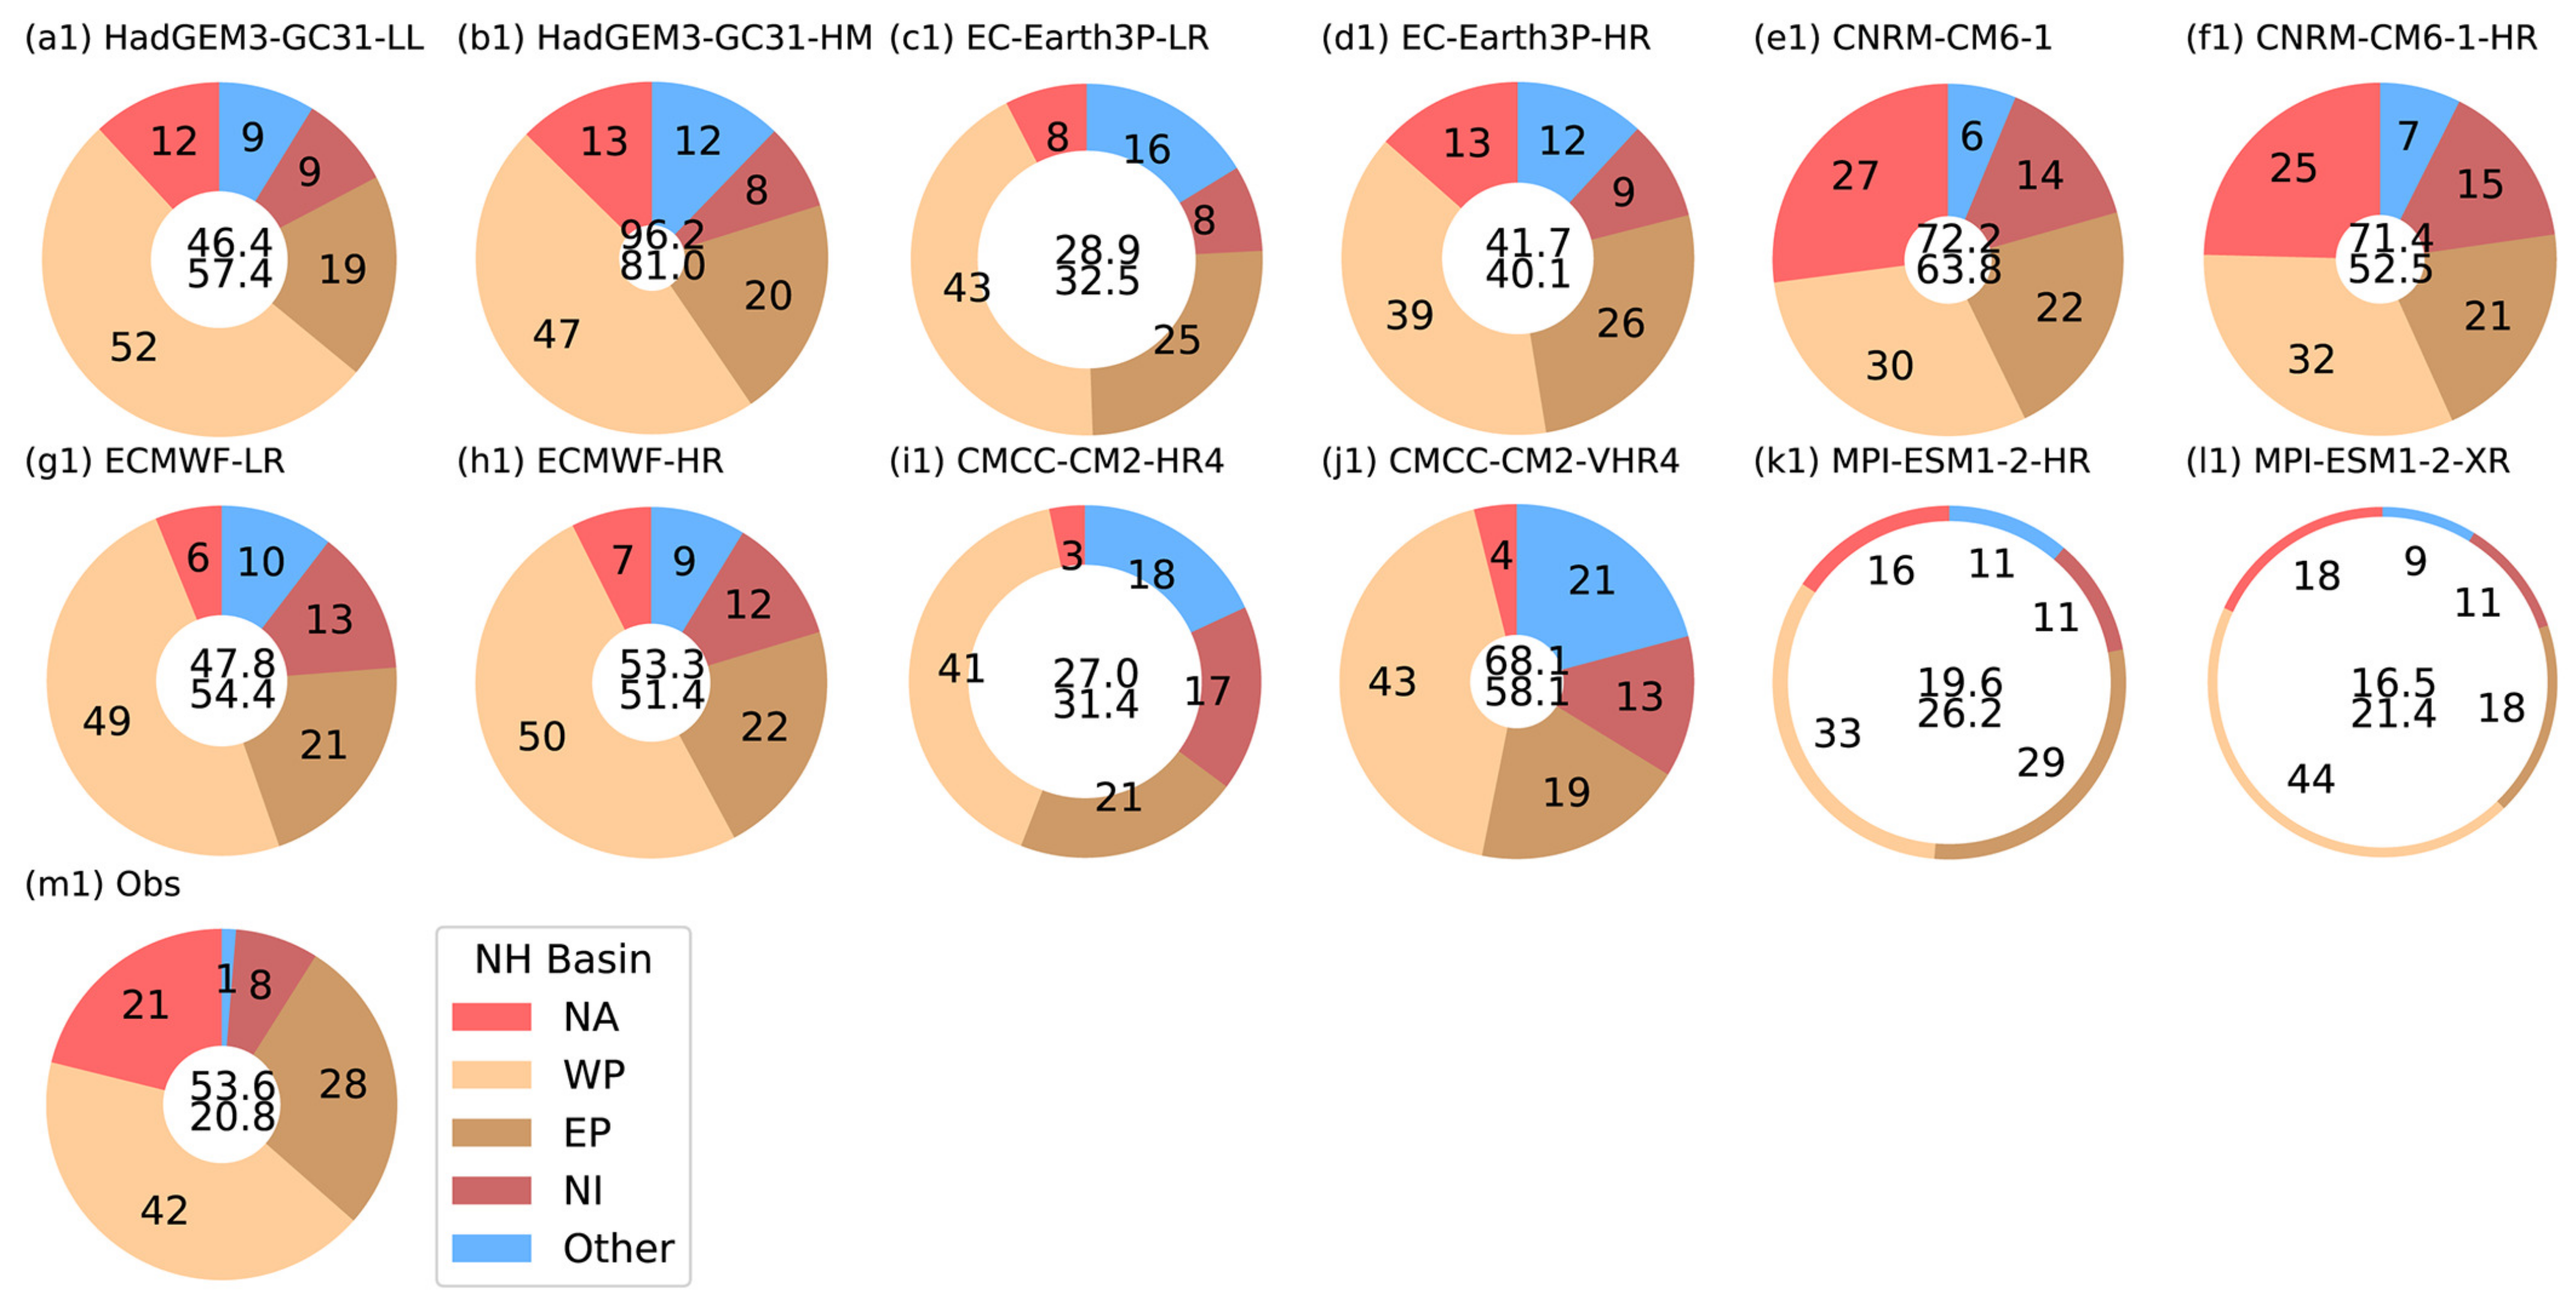
\includegraphics[width=\textwidth]{roberts_projected_2020_TRACKS_coupled.png}
    \caption{Comme pour la \cref{fig:NTC_HighResMIP}, mais où l'algorithme de détection TRACK \parencite{hodges_how_2017} est utilisé à la place de
    TempestExtreme \parencite{ullrich_tempestextremes_2017,zarzycki_assessing_2017}. Les réanalyses ne sont pas incluses. Figure issue de
    \cite{roberts_projected_2020}.}
    \label{fig:NTC_HighResMIP_TRACK}
\end{figure}

Ces différences ne se limitent pas à des biais stationnaires dans le temps ---~auquel cas des traqueurs avec différents résultats en climat présent pourraient
néanmoins indiquer la même tendance relative en climat futur~--- puisque \cite{horn_tracking_2014} ont montré que différents critères de détection peuvent
aboutir à des tendances opposés pour une même expérience. C'est en effet ce que montre la \cref{fig:horn_2014_projections}, avec des changements
relatifs opposés, toutes deux statistiquement significatives à \SI{95}{\percent}, pour le modèle du \textit{Goddard Institute for Space Studies} (GISS) dans
l'expérience à SST accrues (a), pour le traqueur proposé dans \cite{zhao_simulations_2009}, et les tracks obtenues par le groupe du GISS eux-mêmes, selon la
méthodologie de \cite{camargo_improving_2002} ---~deux algorithmes qui, comme beaucoup d'autres, ont pourtant en commun le fait de chercher à diagnostiquer la
présence d'un tourbillon, d'un cœur chaud et d'un minimum local de SLP\footnote{Si la finalité de ces diagnostiques est la même entre les deux méthodes, leurs
implémentations exactes sont toutefois très différentes. Le cas de la méthode de \cite{camargo_improving_2002} est explicité davantage dans la
\cref{sec:intro_chap2}.}. Outre le signe du changement, c'est aussi son amplitude qui se voit affectée par ce choix méthodologique, comme par exemple
pour le cas du modèle GFS (\textit{Global Forecast System}) du \textit{National Centers for Environmental Predictions} (NCEP) et désigné sous cet acronyme dans
la \cref{fig:horn_2014_projections}, en particulier dans les expériences (a) et (b), où la réponse du signal est plus de trois fois supérieures avec le traqueur
de \cite{zhao_simulations_2009} qu'avec le schéma de détection ici nommé CSIRO. Les deux schémas se distinguent l'un de l'autre principalement par le fait que
le premier cherche à identifier un cœur chaud, tandis que le second inclut un seuil de vent minimal à la surface et s'assure également que le vent soit plus
fort dans la basse troposphère que dans les couches supérieures \parencite{horn_tracking_2014}. Les auteurs soulignent que les différences dans les projections
entre les schémas de détection sont amoindries lorsque les critères portant sur la durée minimale, les seuils de vitesses de vents et la latitude de cyclogénèse
sont homogénéisés. Cela illustre donc la difficulté à déterminer les meilleurs critères permettant de discriminer au mieux les HTV d'autres systèmes
météorologiques qui pourraient avoir des caractéristiques similaires ---~comme par exemple les tempêtes extra-tropicales, qui sont une source fréquente de faux
positifs, c'est à dire de systèmes détectés par le schéma de détection qui ne sont pas des cyclones tropicaux (voir aussi \cref{sec:filtrage_mid_latitudes})~--- en faisant toutefois attention à ce que les seuils de détection ne
soient pas trop restrictifs, au risque d'éliminer des systèmes pour de mauvaises raisons.

\begin{figure}[tb]
    \centering
    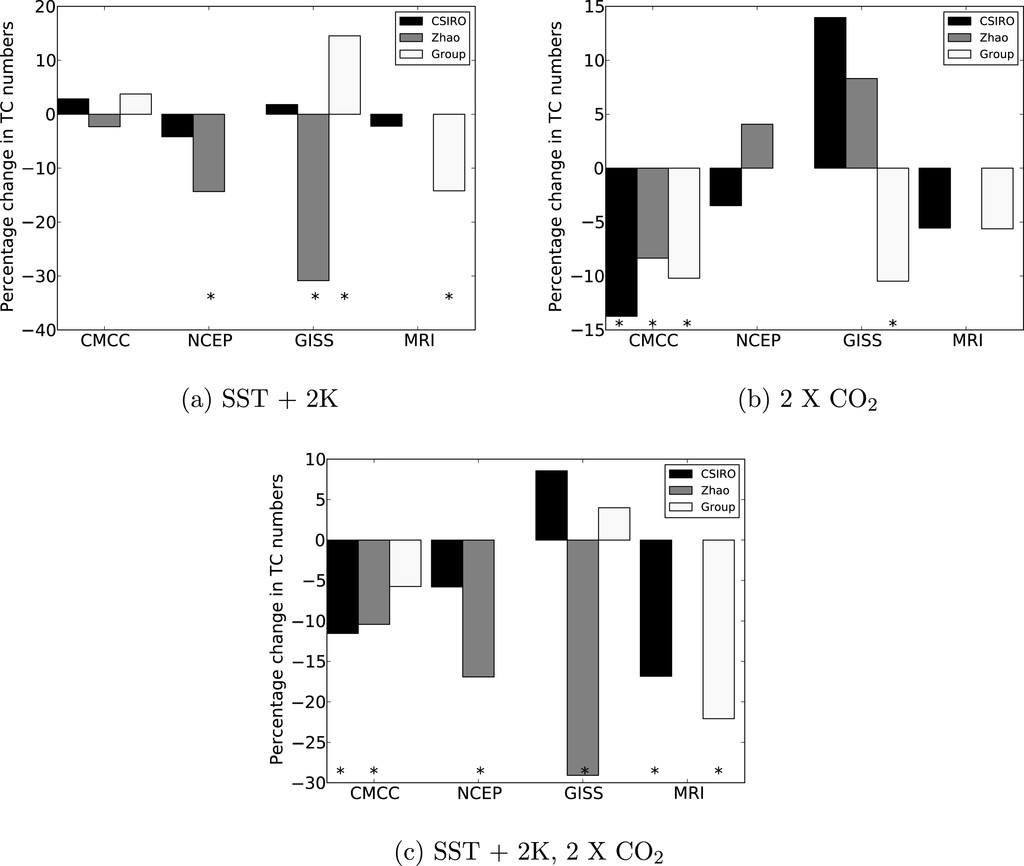
\includegraphics[width=0.9\textwidth]{horn_2014_divergence.jpg}
    \caption{Changements relatifs du nombre moyen annuel de HTV dans quatre modèles (abscisse) et pour différentes méthodologies de tracking (couleurs) dans
    trois expériences à climat altéré notées (a), (b) et (c) par rapport à des simulations du climat présent. Les astérisques indiquent une significativité à
    \SI{95}{\percent}. Figure issue de \cite{horn_tracking_2014}.}
    \label{fig:horn_2014_projections}
\end{figure}

L'approche consistant à appliquer un schéma de détection objective de HTV dans les modèles de climat dans le but d'y mesurer l'activité cyclonique dispose par
conséquent de l'avantage non négligeable de constituer justement une mesure directe. Il est néanmoins important de souligner que la conception de l'algorithme de
détection, ses divers seuils et autres spécificités viennent ajouter autant de sources d'incertitudes qui s'ajoutent aux biais des modèles et leur réponse aux différents scénarios d'évolution du climat.

\subsubsection{Approche indirecte : Indices de cyclogénèse}\label{sec:intro_indices}

Plutôt que de mesurer les HTV directement dans les modèles, l'approche indirecte consiste à inférer l'activité cyclonique en analysant l'environnement de grande
échelle via les variables, ou prédicteurs, associés à cette activité (voir \cref{sec:conditions_cyclogenese}). Pour ce faire, la façon la plus commune consiste à utiliser un indice de cyclogénèse
\parencite{camargo_tropical_2016}. Les indices sont nombreux et tous possèdent des formulations différentes, mais le principe est toujours le même : Un indice de
cyclogénèse combine des prédicteurs thermiques (par exemple la SST, ou l'humidité relative) et des prédicteurs dynamiques (cisaillement, vorticité...) pour
décrire l'environnement favorable à la cyclogénèse et est normalisé, ou calibré, de afin d'être homogène à une quantité de TC ainsi que de reproduire l'amplitude de
l'activité observée sur une période donnée. L'indice peut être alors vu comme un produit indiquant en chaque point de grille un nombre de cyclones par
unité de temps, et s'apparente ainsi à une densité surfacique (puisque le point de grille est représentatif d'une maille du modèle) :
%
\begin{align*}
    N_{\text{TC}} &= \iint\limits_{D} \underbrace{\rho(\phi, \lambda)}_{\text{Indice}} \; d\phi \, d\lambda \\
    \rho &= \underbrace{\vphantom{X_{\text{Dyn}}}A}_{\text{Calibration}} \times \underbrace{\vphantom{X_{\text{Dyn}}}X_{\text{Th}}}_{\text{Thermique}} \times
    \underbrace{X_{\text{Dyn}}}_{\text{Dynamique}}
\end{align*}
%
Où $\rho$ est exprimé sur un domaine géographique $D$ et dépend de la latitude $\phi$ et de la longitude $\lambda$. Comme mentionné dans la
\cref{sec:climato_ingredients}, le premier indice de cyclogénèse a été développé par \cite{gray_tropical_1975}, nommé \textquote{Paramètre de génèse
saisonnière} (\textit{Seasonal Genesis Parameter}, SGP)\footnote{Le SGP de \cite{gray_tropical_1975} consiste en une combinaison de six prédicteurs auxquels
sont ajoutés des constantes déterminées empiriquement et choisies de manière à simuler approximativement les variations journalières de ces variables. La
formulation du SGP est donc plus sophistiquée que le simple produit des quatre variables dont les moyennes saisonnières sont tracées sur la
\cref{fig:produit_ingredients}.}. Comme son nom l'indique, ce dernier est conçu pour prendre en entrée des moyennes saisonnières de ces
prédicteurs. Le SGP tel que défini dans \cite{gray_tropical_1975} s'exprime en TC par boîte de \ang{5}$\times$\ang{5} par 20 ans et est capable de reproduire
fidèlement la densité de cyclones observés sur la période \num{1952}~--~\num{1971}.

L'étude des conditions de grande échelle favorables comme alternative à la mesure directe des HTV était alors particulièrement pertinente dans la mesure où la
résolution des GCM de l'époque ne permettaient pas de les simuler correctement, malgré les résultats encourageants de \cite{broccoli_can_1990} évoqués
précédemment. C'est notamment pour cette raison que \hbox{\cite{ryan_tropical_1992}} ont utilisé pour la première fois le SGP, ainsi qu'une variante annuelle
appelée YGP, dans une expérience \ensuremath{2\times\ce{CO2}} sur des simulations couplées de \num{15} ans. Leurs travaux indiquèrent une très forte
augmentation de la fréquence annuelle de TC ---~passant de \num{149} TC par an\footnote{Cette surévaluation de l'activité cyclonique dans le run de contrôle
(\SI{37}{\percent} de plus que dans \cite{gray_tropical_1975}) est symptomatique d'une absence de re-calibration du SGP lorsque \cite{ryan_tropical_1992}
l'ont appliqué à leur modèle.} dans le run de contrôle à \num{440} TC par an dans le run \ensuremath{2\times\ce{CO2}}, soit une augmentation d'environ
\SI{195}{\percent}~--- accompagnée d'un débordement des zones d'activité dans toutes les directions. Ce résultat s'explique en grande partie par la forte
dépendance du SGP à la SST, leur modèle enregistrant notamment une augmentation de la SST globale moyenne de \SI{4.8}{\degreeCelsius}.
\mbox{\cite{watterson_seasonal_1995}} cherchèrent à évaluer le pouvoir prédictif du SGP à l'échelle saisonnière et inter-annuelle et établirent que l'indice
était capable de reproduire l'effet de l'épisode El Niño de \num{1982}~--~\num{83}, effet visible  aussi bien dans la partie thermique que dynamique de
l'indice, marquée par une augmentation de l'activité dans le Pacifique central. Néanmoins, il notèrent une faible capacité à reproduire la variabilité
inter-annuelle de l'activité dans différents bassins ---~ce qui est encore valable aujourd'hui \parencite{camargo_tropical_2007,camargo_tropical_2016}~--- et
soulignèrent notamment l'amplitude réduite du signal inféré par le SGP par rapport aux observations. La \cref{fig:GP_resolution} issue de
\cite{camargo_tropical_2007} présente l'impact de la résolution du modèle sur la capacité d'un indice à reproduire le cycle annuel de l'activité cyclonique, et
montre une robustesse de la climatologie mensuelle à la résolution. En effet, les auteurs notèrent une augmentation variant de \SI{15}{\percent} à
\SI{50}{\percent} entre les deux extrêmes de résolution, selon le mois et le bassin, avec le passage de \km{310} à \km{210} de résolution présentant le plus
fort impact, puisque les différences sont ensuite moindres jusqu'à la résolution de \km{83}. Cette figure, à travers ses similitudes avec la
\cref{fig:saisons_TC} de la \cref{sec:bassins_saisons}, met également en évidence la capacité de l'indice à reproduire la saisonnalité des bassins océaniques.
\cite{mcdonald_tropical_2005,chauvin_response_2006} montrèrent enfin via des expériences à haute résolution et avec une variante du YGP moins dépendante à la SST
que les indices de cyclogénèse pouvaient apporter de l'information utile quant à l'évolution future de l'activité cyclonique dans des simulations basse
résolution.

\begin{figure}[tb]
    \centering
    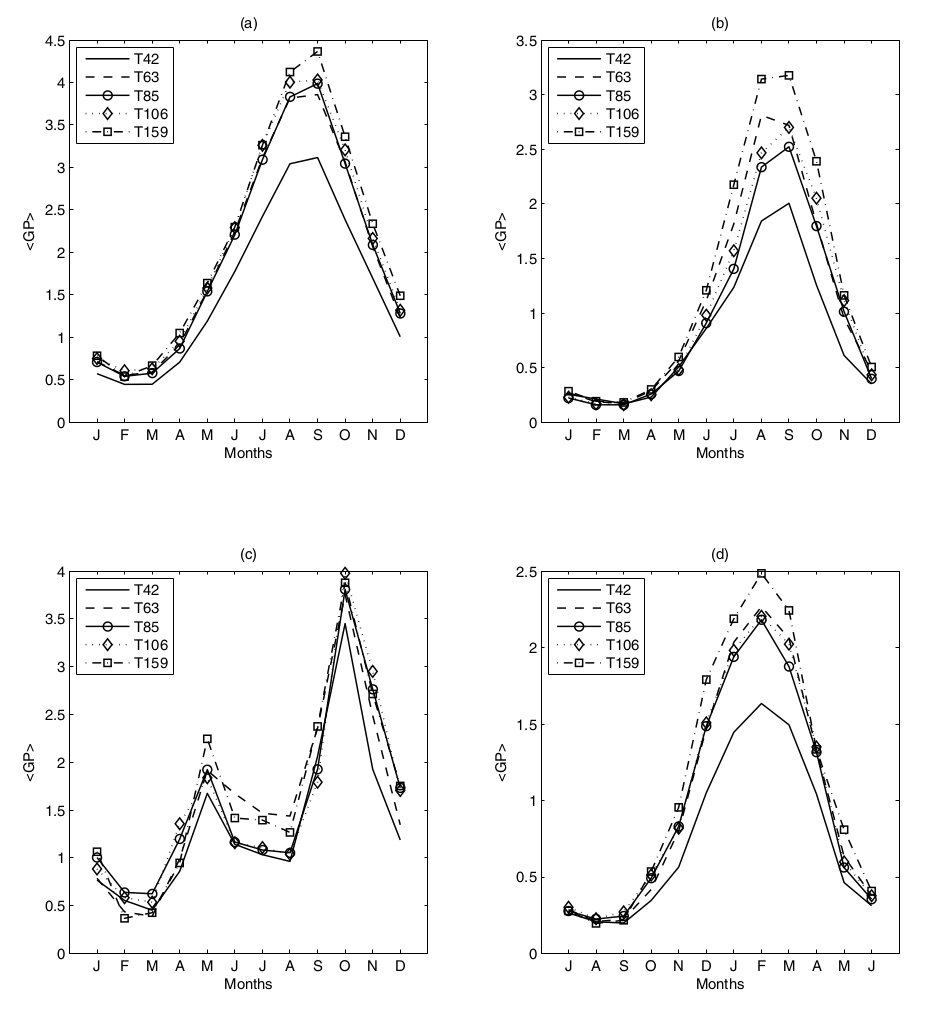
\includegraphics[width=0.8\textwidth]{camargo_tropical_2007_resolution.png}
    \caption{Cycle annuel de l'activité cyclonique inférée par l'indice de cyclogénèse de \cite{emanuel_tropical_2004} dans les bassins WPac (a), NAtl (b), NInd
    (c) et SInd (d) sur la période \num{1978}~--~\num{1999} et à des résolutions de \km{310} (T42), \km{210} (T63), \km{155} (T85), \km{125} (T106) et \km{83}
    (T159) dans le modèle ECHAM5 \parencite{roeckner_atmospheric_2003}. Figure issue de \cite{camargo_tropical_2007}.}
    \label{fig:GP_resolution}
\end{figure}

Ainsi, l'approche indirecte consistant en l'étude de l'environnement de grande échelle favorable à l'activité cyclonique via les indices de cyclogénèse présente
l'intérêt de pouvoir être appliquée à des simulations dont la résolution ne permet pas nécessairement de représenter correctement les TC, et dans lesquelles une
approche directe par détection obejctive serait vraisemblablement sujette à un déficit de TC. Cela représente également une certaine économie, puisque le temps de
calcul est le facteur limitant de la résolution des modèles, et peut aussi se montrer plus facile à appliquer à des simulations diverses issues de modèles
différents que la mise en place d'un schéma de détection homogénéisé. Néanmoins, des incertitudes demeurent sur les poids accordés aux différents prédicteurs,
ainsi que sur le choix des prédicteurs eux-mêmes. De même, l'utilisation d'indices de cyclogénèse pour l'étude de l'activité cyclonique en climat futur suppose
la stationnarité des relations qui sont calibrées sur le climat présent, une hypothèse qui pourrait être erronée, selon
\textcite{nolan_increased_2008,murakami_changes_2013}.

\subsection{Les cyclones dans les projections climatiques}\label{sec:projections_futures}

Les projections futures sur l'activité cyclonique tropicale sont, le plus souvent, issues de grands programmes d'intercomparaison de modèles (MIP). Le plus
notable d'entre eux est sans doute le projet CMIP, dont la plus récente itération (CMIP6) définit un socle commun pour de nombreux autres MIP, comme par exemple
HighResMIP. Ces projets sont définis par une série d'expériences numériques aux protocoles pré-établis et auxquels les divers centres de modélisation à travers
le monde peuvent participer. La mutualisation des données produites par les centres participants constituent alors de grands ensembles que la communauté
scientifique peut ensuite exploiter afin d'étudier divers aspects du système climatique, de sa variabilité interne et de sa sensibilité aux forçages externes. Ainsi, les projections futures des diverses
métriques décrivant l'activité cyclonique présentées ici sont caractérisées par la moyenne (ou la médiane) des résultats issus des groupes travaillant le plus
souvent sur ces ensembles de simulations aux protocoles standardisés, et les incertitudes associées représentent leur dispersion. Les projections les plus à
jour pour les quatre métriques d'intérêt primordial que sont la fréquence d'occurrence des TC, toutes catégories confondues ; la fréquence d'occurrence des TC
les plus forts (catégories 4 et 5 sur l'échelle de Saffir-Simpson) ; L'intensité, exprimée en vitesse maximale de vent à la surface (LMI) et les précipitations
cycloniques sont présentées sur la \cref{fig:projections_TC}. Les projections futures de ces métriques sont commentées ci-dessous, selon leur ordre d'apparition sur la \cref{fig:projections_TC}, en traitant séparément la question de la fréquence des TC toutes catégories confondues des trois autres métriques.
%
\begin{figure}[tb]
    \centering
    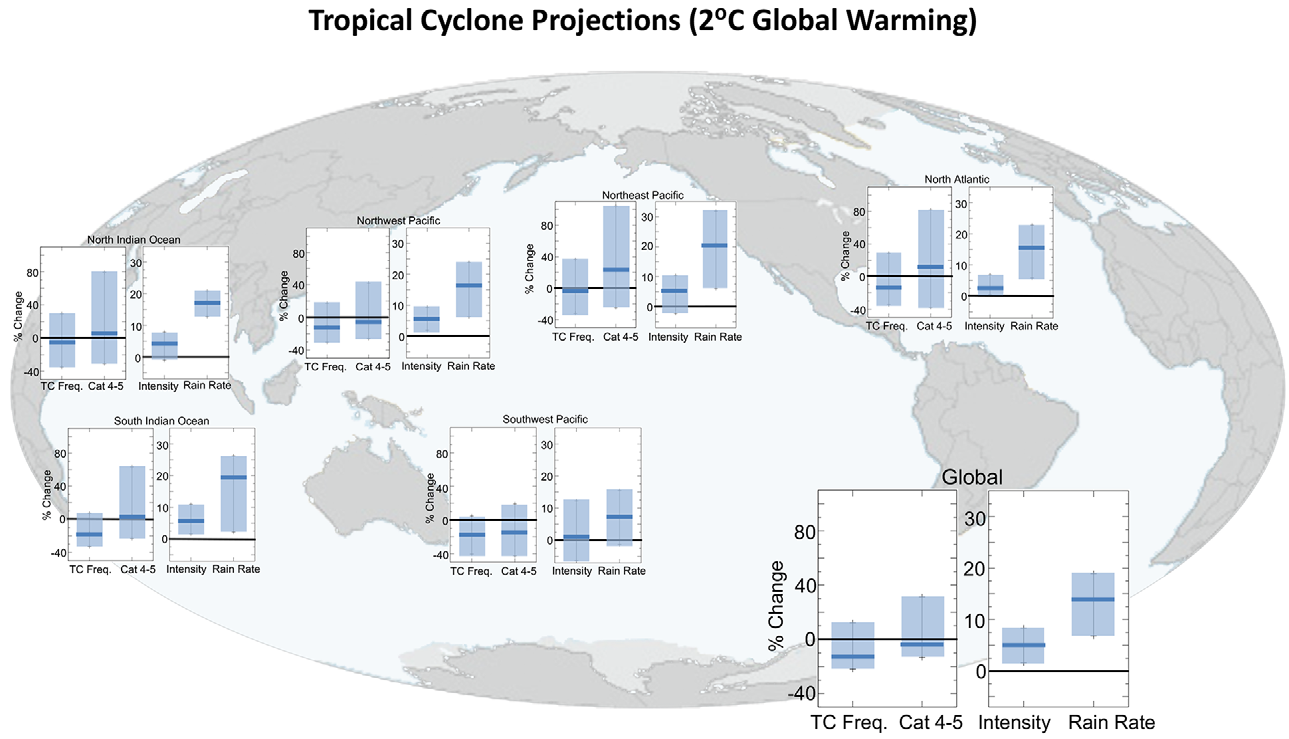
\includegraphics[width=\textwidth]{knutson_2020_projections.png}
    \caption{Résumé des projections simulées du changement de l'activité cyclonique par un réchauffement anthropique de l'atmosphère de \SI{2}{\degreeCelsius} à
        l'échelle globale par rapport à la climatologie \num{1986}~--~\num{2005}, pour les six bassins oćeaniques ainsi qu'à l'échelle du globe. Les changements
        sont exprimés pour la médiane (trait épais) avec son intervalle de confiance construit avec les pourcentiles \SI{5}{\percent}~--~\SI{95}{\percent} pour
        les deux métriques de fréquence, et \SI{10}{\percent}~--~\SI{90}{\percent} pour les métriques d'intensité et de précipitation. Figure issue de
        \cite{knutson_tropical_2020}.}
    \label{fig:projections_TC}
\end{figure}

\subsubsection*{Fréquence d'occurrence}

\begin{figure}[htb]
    \centering
    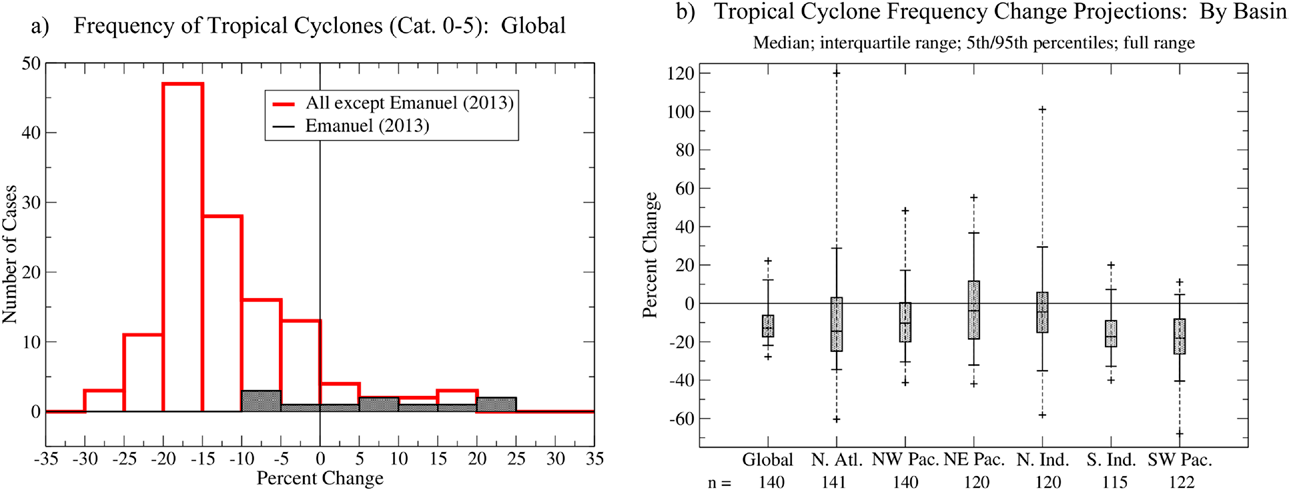
\includegraphics[width=\textwidth]{knutson_2020_TCfreq.png}
    \caption{Synthèse des estimations du changement relatif dans la fréquence d'occurrence des TC toutes catégories dans les \num{59} études utilisées pour ces
        projections, certaines produisant plusieurs estimations, et listées dans \cite[][documents supplémentaires, tableau ES1]{knutson_tropical_2020}, (a) à
        l'échelle globale, où les résultats obtenus par l'approche statistico-dynamique de \cite{emanuel_downscaling_2013} sont séparés des autres études (gris)
        (27 études fournissent des estimations globales). (b) Distributions des changements relatifs dans la fréquence des TC à l'échelle globale et pour chaque
        bassin océanique, incluant \cite{emanuel_downscaling_2013}. Pour (a) comme pour (b), les estimations sont homogénéisées pour être cohérentes avec un
        réchauffement global de \SI{2}{\degreeCelsius} quand nécessaire. Figure issue de \cite{knutson_tropical_2020}.}
    \label{fig:TC_freq_summary}
\end{figure}

La diminution de la fréquence d'occurrence des cyclones tropicaux à l'échelle globale, toutes catégories confondues, constitue un signal robuste du
réchauffement climatique sur l'activité cyclonique, puisque \num{22} des \num{27} études utilisées par \citeauthor{knutson_tropical_2020} présentent un tel signal. Sur la
\cref{fig:TC_freq_summary}.b, le changement médian global est de \SI{-14}{\percent}, avec une plage de valeurs (incluant le minimum et le maximum) allant de
\SI{-28}{\percent} à $+$\SI{22}{\percent}. Le \num{4}\ieme~rapport d'évaluation (AR4) du GIEC (Groupe d'experts intergouvernemental sur l’évolution du climat)
indiquait déjà une possible diminution de l'activité globale, sans avancer de chiffre \parencite{meehl_global_2007}, tandis que l'AR5 concluait à une diminution
probable de l'ordre de \SI{-20}{\percent} \parencite{christensen_climate_2013}. L'AR6 (le dernier en date), quant à lui, reprend les conclusions de
\cite{knutson_tropical_2020} \parencite{seneviratne_weather_2021}, avec donc une baisse moins prononcée de l'ordre de \num{6} points. En effet,
plusieurs équipes ont obtenus, dans certains cas, des résultats indiquant au contraire une augmentation de la fréquence d'occurrence des TC depuis l'AR5
\parencite{camargo_global_2013,emanuel_downscaling_2013,wehner_resolution_2015,bhatia_projected_2018}. Les résultats de \cite{emanuel_downscaling_2013}, basés sur
une méthode combinant un générateur stochastique de trajectoires et une descente d'échelle dynamique, appliqués à des expériences CMIP5 sont présentés sur la
\cref{fig:TC_freq_summary}.a en gris. Ses résultats se situent dans la queue de la distribution, et dépendent de l'hypothèse voulant que la fréquence des
perturbations servant de précurseurs aux TC soit invariante en climat future, ce qui n'est pas vérifiable. Néanmoins, comme \cite{knutson_tropical_2020} le
soulignent, les autres études indiquant une augmentation de l'activité ne sont pas dépendants de cette hypothèse. À l'échelle des bassins océaniques, le signal
est nettement moins robuste et les projections fluctuent d'un bassin à l'autre, avec toutefois les bassins Sud Indien et Sud-ouest Pacifique indiquant une
baisse probable.

Les projections sur le changement dans la fréquence d'occurrence globale présentées sur les \cref{fig:TC_freq_summary,fig:projections_TC} sont basées sur une
approche directe (voir \cref{sec:intro_tracking}). Or, la majorité des travaux appliquant les indices de cyclogénèse à des simulations de changement climatique
indiquent également une augmentation de la fréquence d'occurrence des cyclones tropicaux
\parencite{zhang_changes_2010,emanuel_downscaling_2013,camargo_testing_2014,wehner_resolution_2015,chauvin_future_2020,cattiaux_projected_2020}. Par conséquent,
et bien que la balance penche du côté d'une diminution de l'activité cyclonique, l'incertitude quant au signe du changement persiste. Cette incertitude est par
ailleurs renforcée par l'absence d'un consensus sur le processus physique pouvant expliquer une diminution, avec d'un côté une théorie sur la diminution du flux
de masse ascendant en climat future qui en serait à l'origine \parencite{sugi_decreasing_2012,satoh_constraint_2015}, et de l'autre côté la théorie du déficit
de saturation d'humidité (qui augmente dans une atmosphère plus chaude) \parencite{emanuel_hurricanes_2008,camargo_testing_2014,tang_environmental_2014}. De
même, l'absence de preuves indiquant que les activités humaines aient pu avoir une influence sur la fréquence observée \parencite{knutson_tropical_2019}, ainsi
que le fait que seule l'étude récente de \cite{klotzbach_trends_2022} mesure une tendance à la baisse de la fréquence globale dans les observations, contribuent
à l'incertitude sur le signe du changement de la fréquence des TC dans un climat plus chaud.


\subsubsection*{Fréquence des cyclones forts, intensité maximale et précipitations}

Le changement de fréquence des cyclones les plus forts (catégories 4 et 5 sur l'échelle de Saffir-Simpson) sur la \cref{fig:projections_TC} est ambigu et ni
l'échelle globale, ni les projections locales n'indiquent un changement clair dans cette métrique. Certains bassins ont un changement médian négatif, comme dans
le WPac et SPac, tandis que les autres régions présentent au contraire une médiane positive. L'incertitude est grande dans les deux cas, plus large que celle
sur la fréquence d'occurrence des TC toutes catégories confondues. Une des raisons  à cela réside vraisemblablement dans le fait que ce résultat est sensible
à la résolution des modèles utilisés, puisque \cite{knutson_tropical_2020} soulignent que les modèles de résolution relativement basses (par rapport aux études
considérées, c'est à dire avec des résolutions de l'ordre de \km{50}~--~\km{60}) tendent à indiquer une diminution de la fréquence des TC intenses, tandis que
les modèles à très haute résolution indiquent au contraire une augmentation. En revanche, lorsqu'est considérée la proportion de ces TC, relativement à la
fréquence des TC de toutes catégories (non montré ici), alors les résultats des différentes études convergent nettement vers une intensification, avec une
hausse médiane de \SI{13}{\percent} de la proportion de TC de catégories 4 ou 5 à l'échelle globale sous un scénario de réchauffement de \SI{2}{\degreeCelsius}.
Cette augmentation relative de la fréquence des cyclones les plus forts s'explique par la combinaison de la baisse de la fréquence globale des TC et de
l'augmentation de l'intensité maximale atteinte par les TC dans les projections.

L'augmentation de l'intensité maximale des TC constitue là aussi une réponse
particulièrement robuste de l'activité cyclonique au réchauffement climatique, puisque même les valeurs minimales et maximales de la distribution des résultats
à l'échelle globale sont de même signe, avec une hausse moyenne de l'intensité de \SI{5}{\percent} et comprise entre \SI{1}{\percent} et \SI{10}{\percent}
(respectivement \SI{2}{\percent} et \SI{8}{\percent} pour les pourcentiles \SI{10}{\percent} et \SI{90}{\percent} présentés sur la \cref{fig:projections_TC}).
Localement, seul le bassin le bassin Sud-ouest Pacifique présente une incertitude conséquente sur le signe du changement. La confiance dans ce signal est
renforcée par le fait qu'une tendance à l'intensification est déjà constatée dans les observations (voir \cref{sec:observations}) et qu'il est estimé que les
activités anthropiques y ont contribué \parencite{knutson_tropical_2019}. En outre, une augmentation du LMI dans un climat plus chaud est cohérent avec la
théorie de l'intensité potentielle (\textit{Potential Intensity}, PI) de \cite{emanuel_dependence_1987}.

La \cref{fig:projections_TC} présente le changement relatif dans le débit des précipitations mesurées dans la vicinité des cyclones
tropicaux issus des simulations climatiques. Cette métrique présente le plus grand consensus parmi les quatre présentées sur cette figure, avec notamment
l'ensemble des \num{16} projections utilisées pour quantifier le changement à l'échelle globale indiquant une hausse des précipitations cycloniques comprise
entre \SI{6}{\percent} et \SI{22}{\percent} (respectivement environ \SI{7}{\percent} et \SI{18}{\percent} pour les pourcentiles \SI{10}{\percent} et
\SI{90}{\percent} de la \cref{fig:projections_TC}) et une augmentation médiane de \SI{14}{\percent}. La relation de Clausius-Clapeyron relie la pression de
vapeur saturante à la température de l'air, et permet de montrer que la capacité de l'atmosphère à contenir de la vapeur d'eau augmente d'environ
\SI{7}{\percent} par degré de réchauffement. Une hausse des précipitations cycloniques de \SI{14}{\percent} pour un réchauffement de \SI{2}{\degreeCelsius} est
donc en accord avec cette relation. Le processus physique menant à une augmentation des précipitations cycloniques est par ailleurs bien compris. D'une part,
l'humidité relative est vue comme stable en changement climatique, tandis que la SST et la troposphère se réchauffent, impliquant une augmentation du contenu en
vapeur d'eau de l'atmosphère. De plus, la grande majorité de la vapeur d'eau dans un TC est apportée par la circulation secondaire (radiale, donc convergence
d'humidité). Ainsi, les cyclones tropicaux étant des évènements extrêmes qui mobilisent toute la vapeur d'eau disponible, les précipitations cycloniques sont proportionnelles au contenu en vapeur d'eau de l'atmosphère.

%----------------------------------------------------------------------------------------------------------------------
\section{Synthèse}

Les cyclones tropicaux sont les phénomènes météorologiques les plus violents et les plus dangereux au monde, capables d'atteindre des vitesses de vent soutenus
pouvant aller jusqu'à \kmh{300} et sont responsables de la mort de centaines de milliers de personnes. Les régions les plus à risque sont les zones côtières densément peuplées,
et l'impact des cyclones y est d'autant plus fort que que les pays concernés sont moins développés, tandis que les coûts associés, eux, augmentent avec le
niveau de développement (voir \cref{sec:risques}). Malgré l'enjeu important associé aux TC, le processus de cyclogénèse par lequel les cyclones viennent à se
former est encore incompris, constituant par là même une limite importante à leur prévisibilité. À défaut de comprendre parfaitement le processus, les
conditions de grande échelle favorables à la cyclogénèse sont elles bien connues et impliquent une perturbation initiale, jouant le rôle de précurseur, qui pourra se développer
en cyclone tropical dans une atmosphère instable voire neutre si les conditions de température de surface de l'eau, d'humidité en moyenne troposphère, de cisaillement
vertical du vent et de l'effet de Coriolis sont réunies. La répartition géographique et saisonnière de ces conditions favorables explique en effet la
climatologie observée des cyclones tropicaux (voir \cref{sec:climato_ingredients}). Pour comprendre comment l'activité cyclonique sera affectée par le
réchauffement climatique, dans le but de se donner les moyens de pouvoir s'y préparer, il est nécessaire d'une part de disposer de bases de
données des cyclones tropicaux historiques, afin de pouvoir caractériser le plus précisément possible l'activité présente et les changements qui ont déjà eu
lieu, et d'autre part d'être en mesure de simuler correctement les cyclones tropicaux et l'activité cyclonique associée dans les modèles de climat.

L'analyse de l'activité cyclonique historique dans les bases de données de cyclones est compliquée par la forte hétérogénéité spatiale et temporelle dont souffrent les observations.
L'hétérogénéité temporelle est causée par l'amélioration avec le temps des méthodes d'observation, et particulièrement par l'avènement de l'ère satellitaire à
la fin des années \num{70}, véritable point de rupture technologique pour l'observation météorologique. Par ailleurs, puisque les activités de veille cyclonique
dans chaque bassin d'activité sont sous la responsabilité de centres régionaux spécialisés, eux-mêmes le plus souvent rattachés aux pays concernés, les moyens
affectés à l'observation peuvent varier d'une région à l'autre, causant donc les hétérogénéités spatiales dans les bases de données observées (voir
\cref{sec:observations}). Outre la qualité des données, l'analyse des changements passés dans l'activité cyclonique est également compliquée par les différents
modes de variabilité interne du système climatique qui peuvent affecter les cyclones tropicaux d'une année à l'autre; d'une décennie à l'autre; ou à plus
basse fréquence encore, et ce de manière inégale selon les régions, rendant donc particulièrement difficile la recherche de tendances dans les observations et
les tentatives d'attribution de ces dernières aux activités humaines. Dans les modèles de climat, le principal frein à une représentation précise des cyclones
est leur résolution spatiale. Jusqu'à récemment, la résolution des modèles rendait impossible la simulation de cyclones de catégories \num{4} et \num{5} et tendait
également à produire des cyclones de taille plus importantes que ceux observés. De plus, tous les modèles ne reproduisent pas la climatologie observée des TC,
aussi bien en fréquence annuelle que dans l'activité relative de chaque région, avec des différences plus ou moins importantes selon les modèles (voir
\cref{sec:cyclones_dans_modèles}), causées entre autre par la résolution, mais aussi par la façon dont les composantes atmosphériques et océaniques sont
couplées entre elles, ainsi que par la dynamique et les paramétrisations physiques propres à chaque modèle. À cela s'ajoute une incertitude non négligeable sur
les méthodologies employées pour évaluer l'activité cyclonique dans les modèles. Le choix du schéma de détection et de suivi des cyclones peut avoir
une influence considérable sur l'activité mesurée d'une part, ainsi que sur le signe même du changement dans les projections climatiques d'autre part (voir
\cref{sec:intro_tracking}). Si malgré tout les projections climatiques sur la fréquence d'occurrence des cyclones tropicaux, basées sur les méthodes objectives de détection et de suivi dans les modèles, laissent entrevoir à quelques exceptions près une diminution de la fréquence dans un
climat plus chaud, ce n'est en revanche pas le cas de l'approche indirecte ---~consistant à inférer l'activité indirectement via l'environnement de grande
échelle, avec des indices de cyclogénèse~--- qui tend au contraire à indiquer une tendance à la hausse de la fréquence d'occurrence (voir
\cref{sec:projections_futures}).

C'est précisément sur la différence entre l'approche directe de la détection objective de TC dans les modèles et l'approche indirecte au travers des indices de
cyclogénèse dans les projections climatiques que porte cette thèse. Le \cref{chap:chapitre_2} est ainsi consacré à la détection objective de TC dans les
modèles, avec un tour d'horizon des différents traqueurs employés dans la littérature, avec en particulier une application de l'algorithme de suivi du CNRM à la
réanalyse ERA5 du CEPMMT. Le \cref{chap:chapitre_3} sera consacré aux indices de cyclogénèses, dont un qui sera appliqué sur des simulations ARPEGE en climat
présent. Enfin le \cref{chap:chapitre_4} traitera de l'application à des simulations en climat futur avec ARPEGE en configuration forcée et avec la grille
basculée-étirée.

\end{document}
